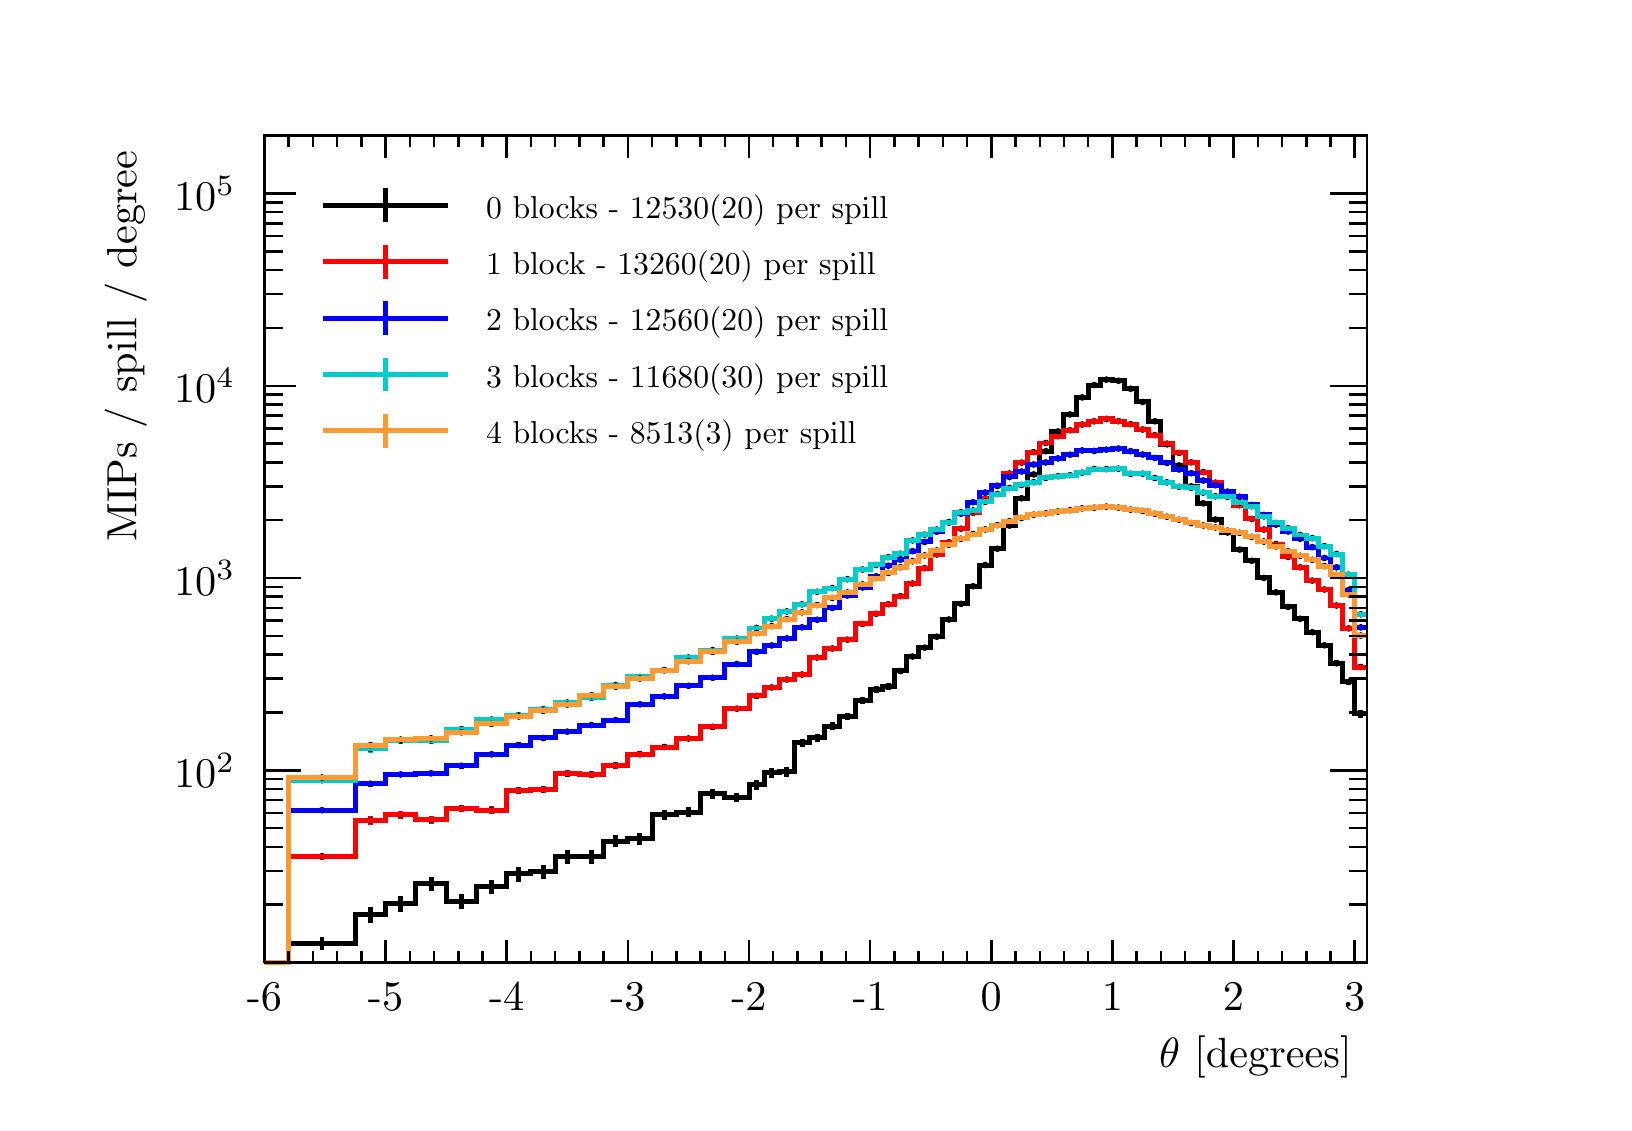
\begin{tikzpicture}
\pgfdeclareplotmark{cross} {
\pgfpathmoveto{\pgfpoint{-0.3\pgfplotmarksize}{\pgfplotmarksize}}
\pgfpathlineto{\pgfpoint{+0.3\pgfplotmarksize}{\pgfplotmarksize}}
\pgfpathlineto{\pgfpoint{+0.3\pgfplotmarksize}{0.3\pgfplotmarksize}}
\pgfpathlineto{\pgfpoint{+1\pgfplotmarksize}{0.3\pgfplotmarksize}}
\pgfpathlineto{\pgfpoint{+1\pgfplotmarksize}{-0.3\pgfplotmarksize}}
\pgfpathlineto{\pgfpoint{+0.3\pgfplotmarksize}{-0.3\pgfplotmarksize}}
\pgfpathlineto{\pgfpoint{+0.3\pgfplotmarksize}{-1.\pgfplotmarksize}}
\pgfpathlineto{\pgfpoint{-0.3\pgfplotmarksize}{-1.\pgfplotmarksize}}
\pgfpathlineto{\pgfpoint{-0.3\pgfplotmarksize}{-0.3\pgfplotmarksize}}
\pgfpathlineto{\pgfpoint{-1.\pgfplotmarksize}{-0.3\pgfplotmarksize}}
\pgfpathlineto{\pgfpoint{-1.\pgfplotmarksize}{0.3\pgfplotmarksize}}
\pgfpathlineto{\pgfpoint{-0.3\pgfplotmarksize}{0.3\pgfplotmarksize}}
\pgfpathclose
\pgfusepathqstroke
}
\pgfdeclareplotmark{cross*} {
\pgfpathmoveto{\pgfpoint{-0.3\pgfplotmarksize}{\pgfplotmarksize}}
\pgfpathlineto{\pgfpoint{+0.3\pgfplotmarksize}{\pgfplotmarksize}}
\pgfpathlineto{\pgfpoint{+0.3\pgfplotmarksize}{0.3\pgfplotmarksize}}
\pgfpathlineto{\pgfpoint{+1\pgfplotmarksize}{0.3\pgfplotmarksize}}
\pgfpathlineto{\pgfpoint{+1\pgfplotmarksize}{-0.3\pgfplotmarksize}}
\pgfpathlineto{\pgfpoint{+0.3\pgfplotmarksize}{-0.3\pgfplotmarksize}}
\pgfpathlineto{\pgfpoint{+0.3\pgfplotmarksize}{-1.\pgfplotmarksize}}
\pgfpathlineto{\pgfpoint{-0.3\pgfplotmarksize}{-1.\pgfplotmarksize}}
\pgfpathlineto{\pgfpoint{-0.3\pgfplotmarksize}{-0.3\pgfplotmarksize}}
\pgfpathlineto{\pgfpoint{-1.\pgfplotmarksize}{-0.3\pgfplotmarksize}}
\pgfpathlineto{\pgfpoint{-1.\pgfplotmarksize}{0.3\pgfplotmarksize}}
\pgfpathlineto{\pgfpoint{-0.3\pgfplotmarksize}{0.3\pgfplotmarksize}}
\pgfpathclose
\pgfusepathqfillstroke
}
\pgfdeclareplotmark{newstar} {
\pgfpathmoveto{\pgfqpoint{0pt}{\pgfplotmarksize}}
\pgfpathlineto{\pgfqpointpolar{44}{0.5\pgfplotmarksize}}
\pgfpathlineto{\pgfqpointpolar{18}{\pgfplotmarksize}}
\pgfpathlineto{\pgfqpointpolar{-20}{0.5\pgfplotmarksize}}
\pgfpathlineto{\pgfqpointpolar{-54}{\pgfplotmarksize}}
\pgfpathlineto{\pgfqpointpolar{-90}{0.5\pgfplotmarksize}}
\pgfpathlineto{\pgfqpointpolar{234}{\pgfplotmarksize}}
\pgfpathlineto{\pgfqpointpolar{198}{0.5\pgfplotmarksize}}
\pgfpathlineto{\pgfqpointpolar{162}{\pgfplotmarksize}}
\pgfpathlineto{\pgfqpointpolar{134}{0.5\pgfplotmarksize}}
\pgfpathclose
\pgfusepathqstroke
}
\pgfdeclareplotmark{newstar*} {
\pgfpathmoveto{\pgfqpoint{0pt}{\pgfplotmarksize}}
\pgfpathlineto{\pgfqpointpolar{44}{0.5\pgfplotmarksize}}
\pgfpathlineto{\pgfqpointpolar{18}{\pgfplotmarksize}}
\pgfpathlineto{\pgfqpointpolar{-20}{0.5\pgfplotmarksize}}
\pgfpathlineto{\pgfqpointpolar{-54}{\pgfplotmarksize}}
\pgfpathlineto{\pgfqpointpolar{-90}{0.5\pgfplotmarksize}}
\pgfpathlineto{\pgfqpointpolar{234}{\pgfplotmarksize}}
\pgfpathlineto{\pgfqpointpolar{198}{0.5\pgfplotmarksize}}
\pgfpathlineto{\pgfqpointpolar{162}{\pgfplotmarksize}}
\pgfpathlineto{\pgfqpointpolar{134}{0.5\pgfplotmarksize}}
\pgfpathclose
\pgfusepathqfillstroke
}
\definecolor{c}{rgb}{1,1,1};
\draw [color=c, fill=c] (0,0) rectangle (20,13.639);
\draw [color=c, fill=c] (3,1.77307) rectangle (17,12.2751);
\definecolor{c}{rgb}{0,0,0};
\draw [c,line width=0.9] (3,1.77307) -- (3,12.2751) -- (17,12.2751) -- (17,1.77307) -- (3,1.77307);
\definecolor{c}{rgb}{1,1,1};
\draw [color=c, fill=c] (3,1.77307) rectangle (17,12.2751);
\definecolor{c}{rgb}{0,0,0};
\draw [c,line width=0.9] (3,1.77307) -- (3,12.2751) -- (17,12.2751) -- (17,1.77307) -- (3,1.77307);
\draw [c,line width=0.9] (3,1.77307) -- (3.30769,1.77307) -- (3.30769,1.77307) -- (4.15385,1.77307) -- (4.15385,1.77307) -- (4.53846,1.77307) -- (4.53846,1.77307) -- (4.92308,1.77307) -- (4.92308,1.77307) -- (5.30769,1.77307) -- (5.30769,1.77307) --
 (5.69231,1.77307) -- (5.69231,1.77307) -- (6.07692,1.77307) -- (6.07692,1.77307) -- (6.38462,1.77307) -- (6.38462,1.77307) -- (6.69231,1.77307) -- (6.69231,1.77307) -- (7,1.77307) -- (7,1.77307) -- (7.30769,1.77307) -- (7.30769,1.77307) --
 (7.61538,1.77307) -- (7.61538,1.77307) -- (7.92308,1.77307) -- (7.92308,1.77307) -- (8.23077,1.77307) -- (8.23077,1.77307) -- (8.53846,1.77307) -- (8.53846,1.77307) -- (8.84615,1.77307) -- (8.84615,1.77307) -- (9.15385,1.77307) -- (9.15385,1.77307)
 -- (9.34615,1.77307) -- (9.34615,1.77307) -- (9.53846,1.77307) -- (9.53846,1.77307) -- (9.73077,1.77307) -- (9.73077,1.77307) -- (9.92308,1.77307) -- (9.92308,1.77307) -- (10.1154,1.77307) -- (10.1154,1.77307) -- (10.3077,1.77307) --
 (10.3077,1.77307) -- (10.5,1.77307) -- (10.5,1.77307) -- (10.6923,1.77307) -- (10.6923,1.77307) -- (10.8462,1.77307) -- (10.8462,1.77307) -- (11,1.77307) -- (11,1.77307) -- (11.1538,1.77307) -- (11.1538,1.77307) -- (11.3077,1.77307) --
 (11.3077,1.77307) -- (11.4615,1.77307) -- (11.4615,1.77307) -- (11.6154,1.77307) -- (11.6154,1.77307) -- (11.7692,1.77307) -- (11.7692,1.77307) -- (11.9231,1.77307) -- (11.9231,1.77307) -- (12.0769,1.77307) -- (12.0769,1.77307) -- (12.2308,1.77307)
 -- (12.2308,1.77307) -- (12.3846,1.77307) -- (12.3846,1.77307) -- (12.5385,1.77307) -- (12.5385,1.77307) -- (12.6923,1.77307) -- (12.6923,1.77307) -- (12.8462,1.77307) -- (12.8462,1.77307) -- (13,1.77307) -- (13,1.77307) -- (13.1538,1.77307) --
 (13.1538,1.77307) -- (13.3077,1.77307) -- (13.3077,1.77307) -- (13.4615,1.77307) -- (13.4615,1.77307) -- (13.6154,1.77307) -- (13.6154,1.77307) -- (13.7692,1.77307) -- (13.7692,1.77307) -- (13.9231,1.77307) -- (13.9231,1.77307) -- (14.0769,1.77307)
 -- (14.0769,1.77307) -- (14.2308,1.77307) -- (14.2308,1.77307) -- (14.3846,1.77307) -- (14.3846,1.77307) -- (14.5385,1.77307) -- (14.5385,1.77307) -- (14.6923,1.77307) -- (14.6923,1.77307) -- (14.8462,1.77307) -- (14.8462,1.77307) -- (15,1.77307) --
 (15,1.77307) -- (15.1538,1.77307) -- (15.1538,1.77307) -- (15.3077,1.77307) -- (15.3077,1.77307) -- (15.4615,1.77307) -- (15.4615,1.77307) -- (15.6154,1.77307) -- (15.6154,1.77307) -- (15.7692,1.77307) -- (15.7692,1.77307) -- (15.9231,1.77307) --
 (15.9231,1.77307) -- (16.0769,1.77307) -- (16.0769,1.77307) -- (16.2308,1.77307) -- (16.2308,1.77307) -- (16.3846,1.77307) -- (16.3846,1.77307) -- (16.5385,1.77307) -- (16.5385,1.77307) -- (16.6923,1.77307) -- (16.6923,1.77307) -- (16.8462,1.77307)
 -- (16.8462,1.77307) -- (17,1.77307);
\draw [c,line width=0.9] (3,1.77307) -- (17,1.77307);
\draw [c,line width=0.9] (3,2.05948) -- (3,1.77307);
\draw [c,line width=0.9] (3.30769,1.91628) -- (3.30769,1.77307);
\draw [c,line width=0.9] (3.61538,1.91628) -- (3.61538,1.77307);
\draw [c,line width=0.9] (3.92308,1.91628) -- (3.92308,1.77307);
\draw [c,line width=0.9] (4.23077,1.91628) -- (4.23077,1.77307);
\draw [c,line width=0.9] (4.53846,2.05948) -- (4.53846,1.77307);
\draw [c,line width=0.9] (4.84615,1.91628) -- (4.84615,1.77307);
\draw [c,line width=0.9] (5.15385,1.91628) -- (5.15385,1.77307);
\draw [c,line width=0.9] (5.46154,1.91628) -- (5.46154,1.77307);
\draw [c,line width=0.9] (5.76923,1.91628) -- (5.76923,1.77307);
\draw [c,line width=0.9] (6.07692,2.05948) -- (6.07692,1.77307);
\draw [c,line width=0.9] (6.38462,1.91628) -- (6.38462,1.77307);
\draw [c,line width=0.9] (6.69231,1.91628) -- (6.69231,1.77307);
\draw [c,line width=0.9] (7,1.91628) -- (7,1.77307);
\draw [c,line width=0.9] (7.30769,1.91628) -- (7.30769,1.77307);
\draw [c,line width=0.9] (7.61538,2.05948) -- (7.61538,1.77307);
\draw [c,line width=0.9] (7.92308,1.91628) -- (7.92308,1.77307);
\draw [c,line width=0.9] (8.23077,1.91628) -- (8.23077,1.77307);
\draw [c,line width=0.9] (8.53846,1.91628) -- (8.53846,1.77307);
\draw [c,line width=0.9] (8.84615,1.91628) -- (8.84615,1.77307);
\draw [c,line width=0.9] (9.15385,2.05948) -- (9.15385,1.77307);
\draw [c,line width=0.9] (9.46154,1.91628) -- (9.46154,1.77307);
\draw [c,line width=0.9] (9.76923,1.91628) -- (9.76923,1.77307);
\draw [c,line width=0.9] (10.0769,1.91628) -- (10.0769,1.77307);
\draw [c,line width=0.9] (10.3846,1.91628) -- (10.3846,1.77307);
\draw [c,line width=0.9] (10.6923,2.05948) -- (10.6923,1.77307);
\draw [c,line width=0.9] (11,1.91628) -- (11,1.77307);
\draw [c,line width=0.9] (11.3077,1.91628) -- (11.3077,1.77307);
\draw [c,line width=0.9] (11.6154,1.91628) -- (11.6154,1.77307);
\draw [c,line width=0.9] (11.9231,1.91628) -- (11.9231,1.77307);
\draw [c,line width=0.9] (12.2308,2.05948) -- (12.2308,1.77307);
\draw [c,line width=0.9] (12.5385,1.91628) -- (12.5385,1.77307);
\draw [c,line width=0.9] (12.8462,1.91628) -- (12.8462,1.77307);
\draw [c,line width=0.9] (13.1538,1.91628) -- (13.1538,1.77307);
\draw [c,line width=0.9] (13.4615,1.91628) -- (13.4615,1.77307);
\draw [c,line width=0.9] (13.7692,2.05948) -- (13.7692,1.77307);
\draw [c,line width=0.9] (14.0769,1.91628) -- (14.0769,1.77307);
\draw [c,line width=0.9] (14.3846,1.91628) -- (14.3846,1.77307);
\draw [c,line width=0.9] (14.6923,1.91628) -- (14.6923,1.77307);
\draw [c,line width=0.9] (15,1.91628) -- (15,1.77307);
\draw [c,line width=0.9] (15.3077,2.05948) -- (15.3077,1.77307);
\draw [c,line width=0.9] (15.6154,1.91628) -- (15.6154,1.77307);
\draw [c,line width=0.9] (15.9231,1.91628) -- (15.9231,1.77307);
\draw [c,line width=0.9] (16.2308,1.91628) -- (16.2308,1.77307);
\draw [c,line width=0.9] (16.5385,1.91628) -- (16.5385,1.77307);
\draw [c,line width=0.9] (16.8462,2.05948) -- (16.8462,1.77307);
\draw [c,line width=0.9] (16.8462,2.05948) -- (16.8462,1.77307);
\draw [anchor=base] (3,1.15931) node[scale=1.52731, color=c, rotate=0]{-6};
\draw [anchor=base] (4.53846,1.15931) node[scale=1.52731, color=c, rotate=0]{-5};
\draw [anchor=base] (6.07692,1.15931) node[scale=1.52731, color=c, rotate=0]{-4};
\draw [anchor=base] (7.61538,1.15931) node[scale=1.52731, color=c, rotate=0]{-3};
\draw [anchor=base] (9.15385,1.15931) node[scale=1.52731, color=c, rotate=0]{-2};
\draw [anchor=base] (10.6923,1.15931) node[scale=1.52731, color=c, rotate=0]{-1};
\draw [anchor=base] (12.2308,1.15931) node[scale=1.52731, color=c, rotate=0]{0};
\draw [anchor=base] (13.7692,1.15931) node[scale=1.52731, color=c, rotate=0]{1};
\draw [anchor=base] (15.3077,1.15931) node[scale=1.52731, color=c, rotate=0]{2};
\draw [anchor=base] (16.8462,1.15931) node[scale=1.52731, color=c, rotate=0]{3};
\draw [anchor= east] (17,0.572837) node[scale=1.52731, color=c, rotate=0]{$\theta$ [degrees] };
\draw [c,line width=0.9] (3,12.2751) -- (17,12.2751);
\draw [c,line width=0.9] (3,11.9887) -- (3,12.2751);
\draw [c,line width=0.9] (3.30769,12.1319) -- (3.30769,12.2751);
\draw [c,line width=0.9] (3.61538,12.1319) -- (3.61538,12.2751);
\draw [c,line width=0.9] (3.92308,12.1319) -- (3.92308,12.2751);
\draw [c,line width=0.9] (4.23077,12.1319) -- (4.23077,12.2751);
\draw [c,line width=0.9] (4.53846,11.9887) -- (4.53846,12.2751);
\draw [c,line width=0.9] (4.84615,12.1319) -- (4.84615,12.2751);
\draw [c,line width=0.9] (5.15385,12.1319) -- (5.15385,12.2751);
\draw [c,line width=0.9] (5.46154,12.1319) -- (5.46154,12.2751);
\draw [c,line width=0.9] (5.76923,12.1319) -- (5.76923,12.2751);
\draw [c,line width=0.9] (6.07692,11.9887) -- (6.07692,12.2751);
\draw [c,line width=0.9] (6.38462,12.1319) -- (6.38462,12.2751);
\draw [c,line width=0.9] (6.69231,12.1319) -- (6.69231,12.2751);
\draw [c,line width=0.9] (7,12.1319) -- (7,12.2751);
\draw [c,line width=0.9] (7.30769,12.1319) -- (7.30769,12.2751);
\draw [c,line width=0.9] (7.61538,11.9887) -- (7.61538,12.2751);
\draw [c,line width=0.9] (7.92308,12.1319) -- (7.92308,12.2751);
\draw [c,line width=0.9] (8.23077,12.1319) -- (8.23077,12.2751);
\draw [c,line width=0.9] (8.53846,12.1319) -- (8.53846,12.2751);
\draw [c,line width=0.9] (8.84615,12.1319) -- (8.84615,12.2751);
\draw [c,line width=0.9] (9.15385,11.9887) -- (9.15385,12.2751);
\draw [c,line width=0.9] (9.46154,12.1319) -- (9.46154,12.2751);
\draw [c,line width=0.9] (9.76923,12.1319) -- (9.76923,12.2751);
\draw [c,line width=0.9] (10.0769,12.1319) -- (10.0769,12.2751);
\draw [c,line width=0.9] (10.3846,12.1319) -- (10.3846,12.2751);
\draw [c,line width=0.9] (10.6923,11.9887) -- (10.6923,12.2751);
\draw [c,line width=0.9] (11,12.1319) -- (11,12.2751);
\draw [c,line width=0.9] (11.3077,12.1319) -- (11.3077,12.2751);
\draw [c,line width=0.9] (11.6154,12.1319) -- (11.6154,12.2751);
\draw [c,line width=0.9] (11.9231,12.1319) -- (11.9231,12.2751);
\draw [c,line width=0.9] (12.2308,11.9887) -- (12.2308,12.2751);
\draw [c,line width=0.9] (12.5385,12.1319) -- (12.5385,12.2751);
\draw [c,line width=0.9] (12.8462,12.1319) -- (12.8462,12.2751);
\draw [c,line width=0.9] (13.1538,12.1319) -- (13.1538,12.2751);
\draw [c,line width=0.9] (13.4615,12.1319) -- (13.4615,12.2751);
\draw [c,line width=0.9] (13.7692,11.9887) -- (13.7692,12.2751);
\draw [c,line width=0.9] (14.0769,12.1319) -- (14.0769,12.2751);
\draw [c,line width=0.9] (14.3846,12.1319) -- (14.3846,12.2751);
\draw [c,line width=0.9] (14.6923,12.1319) -- (14.6923,12.2751);
\draw [c,line width=0.9] (15,12.1319) -- (15,12.2751);
\draw [c,line width=0.9] (15.3077,11.9887) -- (15.3077,12.2751);
\draw [c,line width=0.9] (15.6154,12.1319) -- (15.6154,12.2751);
\draw [c,line width=0.9] (15.9231,12.1319) -- (15.9231,12.2751);
\draw [c,line width=0.9] (16.2308,12.1319) -- (16.2308,12.2751);
\draw [c,line width=0.9] (16.5385,12.1319) -- (16.5385,12.2751);
\draw [c,line width=0.9] (16.8462,11.9887) -- (16.8462,12.2751);
\draw [c,line width=0.9] (16.8462,11.9887) -- (16.8462,12.2751);
\draw [c,line width=0.9] (3,1.77307) -- (3,12.2751);
\draw [c,line width=0.9] (3.231,2.5081) -- (3,2.5081);
\draw [c,line width=0.9] (3.231,2.93807) -- (3,2.93807);
\draw [c,line width=0.9] (3.231,3.24314) -- (3,3.24314);
\draw [c,line width=0.9] (3.231,3.47977) -- (3,3.47977);
\draw [c,line width=0.9] (3.231,3.67311) -- (3,3.67311);
\draw [c,line width=0.9] (3.231,3.83658) -- (3,3.83658);
\draw [c,line width=0.9] (3.231,3.97818) -- (3,3.97818);
\draw [c,line width=0.9] (3.231,4.10308) -- (3,4.10308);
\draw [c,line width=0.9] (3.462,4.21481) -- (3,4.21481);
\draw [anchor= east] (2.82,4.21481) node[scale=1.52731, color=c, rotate=0]{$10^{2}$};
\draw [c,line width=0.9] (3.231,4.94984) -- (3,4.94984);
\draw [c,line width=0.9] (3.231,5.37981) -- (3,5.37981);
\draw [c,line width=0.9] (3.231,5.68488) -- (3,5.68488);
\draw [c,line width=0.9] (3.231,5.92151) -- (3,5.92151);
\draw [c,line width=0.9] (3.231,6.11485) -- (3,6.11485);
\draw [c,line width=0.9] (3.231,6.27832) -- (3,6.27832);
\draw [c,line width=0.9] (3.231,6.41992) -- (3,6.41992);
\draw [c,line width=0.9] (3.231,6.54482) -- (3,6.54482);
\draw [c,line width=0.9] (3.462,6.65655) -- (3,6.65655);
\draw [anchor= east] (2.82,6.65655) node[scale=1.52731, color=c, rotate=0]{$10^{3}$};
\draw [c,line width=0.9] (3.231,7.39159) -- (3,7.39159);
\draw [c,line width=0.9] (3.231,7.82156) -- (3,7.82156);
\draw [c,line width=0.9] (3.231,8.12662) -- (3,8.12662);
\draw [c,line width=0.9] (3.231,8.36325) -- (3,8.36325);
\draw [c,line width=0.9] (3.231,8.55659) -- (3,8.55659);
\draw [c,line width=0.9] (3.231,8.72006) -- (3,8.72006);
\draw [c,line width=0.9] (3.231,8.86166) -- (3,8.86166);
\draw [c,line width=0.9] (3.231,8.98656) -- (3,8.98656);
\draw [c,line width=0.9] (3.462,9.09829) -- (3,9.09829);
\draw [anchor= east] (2.82,9.09829) node[scale=1.52731, color=c, rotate=0]{$10^{4}$};
\draw [c,line width=0.9] (3.231,9.83333) -- (3,9.83333);
\draw [c,line width=0.9] (3.231,10.2633) -- (3,10.2633);
\draw [c,line width=0.9] (3.231,10.5684) -- (3,10.5684);
\draw [c,line width=0.9] (3.231,10.805) -- (3,10.805);
\draw [c,line width=0.9] (3.231,10.9983) -- (3,10.9983);
\draw [c,line width=0.9] (3.231,11.1618) -- (3,11.1618);
\draw [c,line width=0.9] (3.231,11.3034) -- (3,11.3034);
\draw [c,line width=0.9] (3.231,11.4283) -- (3,11.4283);
\draw [c,line width=0.9] (3.462,11.54) -- (3,11.54);
\draw [anchor= east] (2.82,11.54) node[scale=1.52731, color=c, rotate=0]{$10^{5}$};
\draw [c,line width=0.9] (3.231,12.2751) -- (3,12.2751);
\draw [anchor= east] (1.24,12.2751) node[scale=1.52731, color=c, rotate=90]{MIPs / spill / degree};
\draw [c,line width=0.9] (17,1.77307) -- (17,12.2751);
\draw [c,line width=0.9] (16.769,2.5081) -- (17,2.5081);
\draw [c,line width=0.9] (16.769,2.93807) -- (17,2.93807);
\draw [c,line width=0.9] (16.769,3.24314) -- (17,3.24314);
\draw [c,line width=0.9] (16.769,3.47977) -- (17,3.47977);
\draw [c,line width=0.9] (16.769,3.67311) -- (17,3.67311);
\draw [c,line width=0.9] (16.769,3.83658) -- (17,3.83658);
\draw [c,line width=0.9] (16.769,3.97818) -- (17,3.97818);
\draw [c,line width=0.9] (16.769,4.10308) -- (17,4.10308);
\draw [c,line width=0.9] (16.538,4.21481) -- (17,4.21481);
\draw [c,line width=0.9] (16.769,4.94984) -- (17,4.94984);
\draw [c,line width=0.9] (16.769,5.37981) -- (17,5.37981);
\draw [c,line width=0.9] (16.769,5.68488) -- (17,5.68488);
\draw [c,line width=0.9] (16.769,5.92151) -- (17,5.92151);
\draw [c,line width=0.9] (16.769,6.11485) -- (17,6.11485);
\draw [c,line width=0.9] (16.769,6.27832) -- (17,6.27832);
\draw [c,line width=0.9] (16.769,6.41992) -- (17,6.41992);
\draw [c,line width=0.9] (16.769,6.54482) -- (17,6.54482);
\draw [c,line width=0.9] (16.538,6.65655) -- (17,6.65655);
\draw [c,line width=0.9] (16.769,7.39159) -- (17,7.39159);
\draw [c,line width=0.9] (16.769,7.82156) -- (17,7.82156);
\draw [c,line width=0.9] (16.769,8.12662) -- (17,8.12662);
\draw [c,line width=0.9] (16.769,8.36325) -- (17,8.36325);
\draw [c,line width=0.9] (16.769,8.55659) -- (17,8.55659);
\draw [c,line width=0.9] (16.769,8.72006) -- (17,8.72006);
\draw [c,line width=0.9] (16.769,8.86166) -- (17,8.86166);
\draw [c,line width=0.9] (16.769,8.98656) -- (17,8.98656);
\draw [c,line width=0.9] (16.538,9.09829) -- (17,9.09829);
\draw [c,line width=0.9] (16.769,9.83333) -- (17,9.83333);
\draw [c,line width=0.9] (16.769,10.2633) -- (17,10.2633);
\draw [c,line width=0.9] (16.769,10.5684) -- (17,10.5684);
\draw [c,line width=0.9] (16.769,10.805) -- (17,10.805);
\draw [c,line width=0.9] (16.769,10.9983) -- (17,10.9983);
\draw [c,line width=0.9] (16.769,11.1618) -- (17,11.1618);
\draw [c,line width=0.9] (16.769,11.3034) -- (17,11.3034);
\draw [c,line width=0.9] (16.769,11.4283) -- (17,11.4283);
\draw [c,line width=0.9] (16.538,11.54) -- (17,11.54);
\draw [c,line width=0.9] (16.769,12.2751) -- (17,12.2751);
\draw [c,line width=1.8] (3.73077,1.92614) -- (3.73077,2.01524);
\draw [c,line width=1.8] (3.73077,2.01524) -- (3.73077,2.09743);
\foreach \P in {(3.73077,2.01524)}{\draw[mark options={color=c,fill=c},mark size=2.402402pt,mark=*,mark size=1pt] plot coordinates {\P};}
\draw [c,line width=1.8] (4.34615,2.27048) -- (4.34615,2.38281);
\draw [c,line width=1.8] (4.34615,2.38281) -- (4.34615,2.48437);
\foreach \P in {(4.34615,2.38281)}{\draw[mark options={color=c,fill=c},mark size=2.402402pt,mark=*,mark size=1pt] plot coordinates {\P};}
\draw [c,line width=1.8] (4.73077,2.4183) -- (4.73077,2.52307);
\draw [c,line width=1.8] (4.73077,2.52307) -- (4.73077,2.61842);
\foreach \P in {(4.73077,2.52307)}{\draw[mark options={color=c,fill=c},mark size=2.402402pt,mark=*,mark size=1pt] plot coordinates {\P};}
\draw [c,line width=1.8] (5.11538,2.68015) -- (5.11538,2.77276);
\draw [c,line width=1.8] (5.11538,2.77276) -- (5.11538,2.85793);
\foreach \P in {(5.11538,2.77276)}{\draw[mark options={color=c,fill=c},mark size=2.402402pt,mark=*,mark size=1pt] plot coordinates {\P};}
\draw [c,line width=1.8] (5.5,2.44752) -- (5.5,2.55086);
\draw [c,line width=1.8] (5.5,2.55086) -- (5.5,2.64502);
\foreach \P in {(5.5,2.55086)}{\draw[mark options={color=c,fill=c},mark size=2.402402pt,mark=*,mark size=1pt] plot coordinates {\P};}
\draw [c,line width=1.8] (5.88462,2.64067) -- (5.88462,2.73502);
\draw [c,line width=1.8] (5.88462,2.73502) -- (5.88462,2.82166);
\foreach \P in {(5.88462,2.73502)}{\draw[mark options={color=c,fill=c},mark size=2.402402pt,mark=*,mark size=1pt] plot coordinates {\P};}
\draw [c,line width=1.8] (6.23077,2.80239) -- (6.23077,2.90013);
\draw [c,line width=1.8] (6.23077,2.90013) -- (6.23077,2.98962);
\foreach \P in {(6.23077,2.90013)}{\draw[mark options={color=c,fill=c},mark size=2.402402pt,mark=*,mark size=1pt] plot coordinates {\P};}
\draw [c,line width=1.8] (6.53846,2.82794) -- (6.53846,2.92451);
\draw [c,line width=1.8] (6.53846,2.92451) -- (6.53846,3.01301);
\foreach \P in {(6.53846,2.92451)}{\draw[mark options={color=c,fill=c},mark size=2.402402pt,mark=*,mark size=1pt] plot coordinates {\P};}
\draw [c,line width=1.8] (6.84615,3.02725) -- (6.84615,3.11517);
\draw [c,line width=1.8] (6.84615,3.11517) -- (6.84615,3.19635);
\foreach \P in {(6.84615,3.11517)}{\draw[mark options={color=c,fill=c},mark size=2.402402pt,mark=*,mark size=1pt] plot coordinates {\P};}
\draw [c,line width=1.8] (7.15385,3.02725) -- (7.15385,3.11517);
\draw [c,line width=1.8] (7.15385,3.11517) -- (7.15385,3.19635);
\foreach \P in {(7.15385,3.11517)}{\draw[mark options={color=c,fill=c},mark size=2.402402pt,mark=*,mark size=1pt] plot coordinates {\P};}
\draw [c,line width=1.8] (7.46154,3.23666) -- (7.46154,3.31631);
\draw [c,line width=1.8] (7.46154,3.31631) -- (7.46154,3.39039);
\foreach \P in {(7.46154,3.31631)}{\draw[mark options={color=c,fill=c},mark size=2.402402pt,mark=*,mark size=1pt] plot coordinates {\P};}
\draw [c,line width=1.8] (7.76923,3.27072) -- (7.76923,3.34911);
\draw [c,line width=1.8] (7.76923,3.34911) -- (7.76923,3.4221);
\foreach \P in {(7.76923,3.34911)}{\draw[mark options={color=c,fill=c},mark size=2.402402pt,mark=*,mark size=1pt] plot coordinates {\P};}
\draw [c,line width=1.8] (8.07692,3.58385) -- (8.07692,3.65148);
\draw [c,line width=1.8] (8.07692,3.65148) -- (8.07692,3.71506);
\foreach \P in {(8.07692,3.65148)}{\draw[mark options={color=c,fill=c},mark size=2.402402pt,mark=*,mark size=1pt] plot coordinates {\P};}
\draw [c,line width=1.8] (8.38461,3.61679) -- (8.38461,3.68338);
\draw [c,line width=1.8] (8.38461,3.68338) -- (8.38461,3.74603);
\foreach \P in {(8.38461,3.68338)}{\draw[mark options={color=c,fill=c},mark size=2.402402pt,mark=*,mark size=1pt] plot coordinates {\P};}
\draw [c,line width=1.8] (8.69231,3.85579) -- (8.69231,3.91528);
\draw [c,line width=1.8] (8.69231,3.91528) -- (8.69231,3.97161);
\foreach \P in {(8.69231,3.91528)}{\draw[mark options={color=c,fill=c},mark size=2.402402pt,mark=*,mark size=1pt] plot coordinates {\P};}
\draw [c,line width=1.8] (9,3.80594) -- (9,3.86685);
\draw [c,line width=1.8] (9,3.86685) -- (9,3.92445);
\foreach \P in {(9,3.86685)}{\draw[mark options={color=c,fill=c},mark size=2.402402pt,mark=*,mark size=1pt] plot coordinates {\P};}
\draw [c,line width=1.8] (9.25,3.95834) -- (9.25,4.03004);
\draw [c,line width=1.8] (9.25,4.03004) -- (9.25,4.09719);
\foreach \P in {(9.25,4.03004)}{\draw[mark options={color=c,fill=c},mark size=2.402402pt,mark=*,mark size=1pt] plot coordinates {\P};}
\draw [c,line width=1.8] (9.44231,4.1152) -- (9.44231,4.18179);
\draw [c,line width=1.8] (9.44231,4.18179) -- (9.44231,4.24444);
\foreach \P in {(9.44231,4.18179)}{\draw[mark options={color=c,fill=c},mark size=2.402402pt,mark=*,mark size=1pt] plot coordinates {\P};}
\draw [c,line width=1.8] (9.63461,4.12729) -- (9.63461,4.1935);
\draw [c,line width=1.8] (9.63461,4.1935) -- (9.63461,4.25582);
\foreach \P in {(9.63461,4.1935)}{\draw[mark options={color=c,fill=c},mark size=2.402402pt,mark=*,mark size=1pt] plot coordinates {\P};}
\draw [c,line width=1.8] (9.82692,4.50822) -- (9.82692,4.56354);
\draw [c,line width=1.8] (9.82692,4.56354) -- (9.82692,4.61613);
\foreach \P in {(9.82692,4.56354)}{\draw[mark options={color=c,fill=c},mark size=2.402402pt,mark=*,mark size=1pt] plot coordinates {\P};}
\draw [c,line width=1.8] (10.0192,4.57635) -- (10.0192,4.62993);
\draw [c,line width=1.8] (10.0192,4.62993) -- (10.0192,4.68093);
\foreach \P in {(10.0192,4.62993)}{\draw[mark options={color=c,fill=c},mark size=2.402402pt,mark=*,mark size=1pt] plot coordinates {\P};}
\draw [c,line width=1.8] (10.2115,4.72413) -- (10.2115,4.7741);
\draw [c,line width=1.8] (10.2115,4.7741) -- (10.2115,4.82182);
\foreach \P in {(10.2115,4.7741)}{\draw[mark options={color=c,fill=c},mark size=2.402402pt,mark=*,mark size=1pt] plot coordinates {\P};}
\draw [c,line width=1.8] (10.4038,4.84991) -- (10.4038,4.897);
\draw [c,line width=1.8] (10.4038,4.897) -- (10.4038,4.94209);
\foreach \P in {(10.4038,4.897)}{\draw[mark options={color=c,fill=c},mark size=2.402402pt,mark=*,mark size=1pt] plot coordinates {\P};}
\draw [c,line width=1.8] (10.5962,5.06096) -- (10.5962,5.1036);
\draw [c,line width=1.8] (10.5962,5.1036) -- (10.5962,5.14458);
\foreach \P in {(10.5962,5.1036)}{\draw[mark options={color=c,fill=c},mark size=2.402402pt,mark=*,mark size=1pt] plot coordinates {\P};}
\draw [c,line width=1.8] (10.7692,5.1954) -- (10.7692,5.24014);
\draw [c,line width=1.8] (10.7692,5.24014) -- (10.7692,5.28307);
\foreach \P in {(10.7692,5.24014)}{\draw[mark options={color=c,fill=c},mark size=2.402402pt,mark=*,mark size=1pt] plot coordinates {\P};}
\draw [c,line width=1.8] (10.9231,5.2371) -- (10.9231,5.28097);
\draw [c,line width=1.8] (10.9231,5.28097) -- (10.9231,5.32309);
\foreach \P in {(10.9231,5.28097)}{\draw[mark options={color=c,fill=c},mark size=2.402402pt,mark=*,mark size=1pt] plot coordinates {\P};}
\draw [c,line width=1.8] (11.0769,5.43611) -- (11.0769,5.47605);
\draw [c,line width=1.8] (11.0769,5.47605) -- (11.0769,5.51454);
\foreach \P in {(11.0769,5.47605)}{\draw[mark options={color=c,fill=c},mark size=2.402402pt,mark=*,mark size=1pt] plot coordinates {\P};}
\draw [c,line width=1.8] (11.2308,5.62262) -- (11.2308,5.6592);
\draw [c,line width=1.8] (11.2308,5.6592) -- (11.2308,5.69456);
\foreach \P in {(11.2308,5.6592)}{\draw[mark options={color=c,fill=c},mark size=2.402402pt,mark=*,mark size=1pt] plot coordinates {\P};}
\draw [c,line width=1.8] (11.3846,5.73774) -- (11.3846,5.77239);
\draw [c,line width=1.8] (11.3846,5.77239) -- (11.3846,5.80594);
\foreach \P in {(11.3846,5.77239)}{\draw[mark options={color=c,fill=c},mark size=2.402402pt,mark=*,mark size=1pt] plot coordinates {\P};}
\draw [c,line width=1.8] (11.5385,5.87841) -- (11.5385,5.91084);
\draw [c,line width=1.8] (11.5385,5.91084) -- (11.5385,5.9423);
\foreach \P in {(11.5385,5.91084)}{\draw[mark options={color=c,fill=c},mark size=2.402402pt,mark=*,mark size=1pt] plot coordinates {\P};}
\draw [c,line width=1.8] (11.6923,6.10062) -- (11.6923,6.12982);
\draw [c,line width=1.8] (11.6923,6.12982) -- (11.6923,6.15824);
\foreach \P in {(11.6923,6.12982)}{\draw[mark options={color=c,fill=c},mark size=2.402402pt,mark=*,mark size=1pt] plot coordinates {\P};}
\draw [c,line width=1.8] (11.8462,6.30168) -- (11.8462,6.32823);
\draw [c,line width=1.8] (11.8462,6.32823) -- (11.8462,6.35414);
\foreach \P in {(11.8462,6.32823)}{\draw[mark options={color=c,fill=c},mark size=2.402402pt,mark=*,mark size=1pt] plot coordinates {\P};}
\draw [c,line width=1.8] (12,6.5286) -- (12,6.55247);
\draw [c,line width=1.8] (12,6.55247) -- (12,6.5758);
\foreach \P in {(12,6.55247)}{\draw[mark options={color=c,fill=c},mark size=2.402402pt,mark=*,mark size=1pt] plot coordinates {\P};}
\draw [c,line width=1.8] (12.1538,6.80078) -- (12.1538,6.82177);
\draw [c,line width=1.8] (12.1538,6.82177) -- (12.1538,6.84235);
\foreach \P in {(12.1538,6.82177)}{\draw[mark options={color=c,fill=c},mark size=2.402402pt,mark=*,mark size=1pt] plot coordinates {\P};}
\draw [c,line width=1.8] (12.3077,7.00964) -- (12.3077,7.02866);
\draw [c,line width=1.8] (12.3077,7.02866) -- (12.3077,7.04735);
\foreach \P in {(12.3077,7.02866)}{\draw[mark options={color=c,fill=c},mark size=2.402402pt,mark=*,mark size=1pt] plot coordinates {\P};}
\draw [c,line width=1.8] (12.4615,7.30582) -- (12.4615,7.32236);
\draw [c,line width=1.8] (12.4615,7.32236) -- (12.4615,7.33865);
\foreach \P in {(12.4615,7.32236)}{\draw[mark options={color=c,fill=c},mark size=2.402402pt,mark=*,mark size=1pt] plot coordinates {\P};}
\draw [c,line width=1.8] (12.6154,7.65548) -- (12.6154,7.66951);
\draw [c,line width=1.8] (12.6154,7.66951) -- (12.6154,7.68335);
\foreach \P in {(12.6154,7.66951)}{\draw[mark options={color=c,fill=c},mark size=2.402402pt,mark=*,mark size=1pt] plot coordinates {\P};}
\draw [c,line width=1.8] (12.7692,7.96041) -- (12.7692,7.97256);
\draw [c,line width=1.8] (12.7692,7.97256) -- (12.7692,7.98457);
\foreach \P in {(12.7692,7.97256)}{\draw[mark options={color=c,fill=c},mark size=2.402402pt,mark=*,mark size=1pt] plot coordinates {\P};}
\draw [c,line width=1.8] (12.9231,8.25708) -- (12.9231,8.26764);
\draw [c,line width=1.8] (12.9231,8.26764) -- (12.9231,8.2781);
\foreach \P in {(12.9231,8.26764)}{\draw[mark options={color=c,fill=c},mark size=2.402402pt,mark=*,mark size=1pt] plot coordinates {\P};}
\draw [c,line width=1.8] (13.0769,8.50812) -- (13.0769,8.5175);
\draw [c,line width=1.8] (13.0769,8.5175) -- (13.0769,8.5268);
\foreach \P in {(13.0769,8.5175)}{\draw[mark options={color=c,fill=c},mark size=2.402402pt,mark=*,mark size=1pt] plot coordinates {\P};}
\draw [c,line width=1.8] (13.2308,8.72542) -- (13.2308,8.73389);
\draw [c,line width=1.8] (13.2308,8.73389) -- (13.2308,8.74229);
\foreach \P in {(13.2308,8.73389)}{\draw[mark options={color=c,fill=c},mark size=2.402402pt,mark=*,mark size=1pt] plot coordinates {\P};}
\draw [c,line width=1.8] (13.3846,8.94273) -- (13.3846,8.95037);
\draw [c,line width=1.8] (13.3846,8.95037) -- (13.3846,8.95796);
\foreach \P in {(13.3846,8.95037)}{\draw[mark options={color=c,fill=c},mark size=2.402402pt,mark=*,mark size=1pt] plot coordinates {\P};}
\draw [c,line width=1.8] (13.5385,9.10047) -- (13.5385,9.10757);
\draw [c,line width=1.8] (13.5385,9.10757) -- (13.5385,9.11462);
\foreach \P in {(13.5385,9.10757)}{\draw[mark options={color=c,fill=c},mark size=2.402402pt,mark=*,mark size=1pt] plot coordinates {\P};}
\draw [c,line width=1.8] (13.6923,9.16942) -- (13.6923,9.17629);
\draw [c,line width=1.8] (13.6923,9.17629) -- (13.6923,9.18312);
\foreach \P in {(13.6923,9.17629)}{\draw[mark options={color=c,fill=c},mark size=2.402402pt,mark=*,mark size=1pt] plot coordinates {\P};}
\draw [c,line width=1.8] (13.8462,9.15504) -- (13.8462,9.16196);
\draw [c,line width=1.8] (13.8462,9.16196) -- (13.8462,9.16883);
\foreach \P in {(13.8462,9.16196)}{\draw[mark options={color=c,fill=c},mark size=2.402402pt,mark=*,mark size=1pt] plot coordinates {\P};}
\draw [c,line width=1.8] (14,9.0526) -- (14,9.05985);
\draw [c,line width=1.8] (14,9.05985) -- (14,9.06706);
\foreach \P in {(14,9.05985)}{\draw[mark options={color=c,fill=c},mark size=2.402402pt,mark=*,mark size=1pt] plot coordinates {\P};}
\draw [c,line width=1.8] (14.1538,8.88426) -- (14.1538,8.89212);
\draw [c,line width=1.8] (14.1538,8.89212) -- (14.1538,8.89992);
\foreach \P in {(14.1538,8.89212)}{\draw[mark options={color=c,fill=c},mark size=2.402402pt,mark=*,mark size=1pt] plot coordinates {\P};}
\draw [c,line width=1.8] (14.3077,8.63878) -- (14.3077,8.6476);
\draw [c,line width=1.8] (14.3077,8.6476) -- (14.3077,8.65635);
\foreach \P in {(14.3077,8.6476)}{\draw[mark options={color=c,fill=c},mark size=2.402402pt,mark=*,mark size=1pt] plot coordinates {\P};}
\draw [c,line width=1.8] (14.4615,8.34369) -- (14.4615,8.35383);
\draw [c,line width=1.8] (14.4615,8.35383) -- (14.4615,8.36387);
\foreach \P in {(14.4615,8.35383)}{\draw[mark options={color=c,fill=c},mark size=2.402402pt,mark=*,mark size=1pt] plot coordinates {\P};}
\draw [c,line width=1.8] (14.6154,8.07483) -- (14.6154,8.08634);
\draw [c,line width=1.8] (14.6154,8.08634) -- (14.6154,8.09772);
\foreach \P in {(14.6154,8.08634)}{\draw[mark options={color=c,fill=c},mark size=2.402402pt,mark=*,mark size=1pt] plot coordinates {\P};}
\draw [c,line width=1.8] (14.7692,7.80771) -- (14.7692,7.82077);
\draw [c,line width=1.8] (14.7692,7.82077) -- (14.7692,7.83367);
\foreach \P in {(14.7692,7.82077)}{\draw[mark options={color=c,fill=c},mark size=2.402402pt,mark=*,mark size=1pt] plot coordinates {\P};}
\draw [c,line width=1.8] (14.9231,7.5909) -- (14.9231,7.60536);
\draw [c,line width=1.8] (14.9231,7.60536) -- (14.9231,7.61962);
\foreach \P in {(14.9231,7.60536)}{\draw[mark options={color=c,fill=c},mark size=2.402402pt,mark=*,mark size=1pt] plot coordinates {\P};}
\draw [c,line width=1.8] (15.0769,7.38355) -- (15.0769,7.39949);
\draw [c,line width=1.8] (15.0769,7.39949) -- (15.0769,7.4152);
\foreach \P in {(15.0769,7.39949)}{\draw[mark options={color=c,fill=c},mark size=2.402402pt,mark=*,mark size=1pt] plot coordinates {\P};}
\draw [c,line width=1.8] (15.2308,7.21725) -- (15.2308,7.23449);
\draw [c,line width=1.8] (15.2308,7.23449) -- (15.2308,7.25146);
\foreach \P in {(15.2308,7.23449)}{\draw[mark options={color=c,fill=c},mark size=2.402402pt,mark=*,mark size=1pt] plot coordinates {\P};}
\draw [c,line width=1.8] (15.3846,6.99877) -- (15.3846,7.01788);
\draw [c,line width=1.8] (15.3846,7.01788) -- (15.3846,7.03666);
\foreach \P in {(15.3846,7.01788)}{\draw[mark options={color=c,fill=c},mark size=2.402402pt,mark=*,mark size=1pt] plot coordinates {\P};}
\draw [c,line width=1.8] (15.5385,6.85451) -- (15.5385,6.87498);
\draw [c,line width=1.8] (15.5385,6.87498) -- (15.5385,6.89505);
\foreach \P in {(15.5385,6.87498)}{\draw[mark options={color=c,fill=c},mark size=2.402402pt,mark=*,mark size=1pt] plot coordinates {\P};}
\draw [c,line width=1.8] (15.6923,6.63513) -- (15.6923,6.65782);
\draw [c,line width=1.8] (15.6923,6.65782) -- (15.6923,6.68004);
\foreach \P in {(15.6923,6.65782)}{\draw[mark options={color=c,fill=c},mark size=2.402402pt,mark=*,mark size=1pt] plot coordinates {\P};}
\draw [c,line width=1.8] (15.8462,6.45041) -- (15.8462,6.47517);
\draw [c,line width=1.8] (15.8462,6.47517) -- (15.8462,6.49936);
\foreach \P in {(15.8462,6.47517)}{\draw[mark options={color=c,fill=c},mark size=2.402402pt,mark=*,mark size=1pt] plot coordinates {\P};}
\draw [c,line width=1.8] (16,6.2622) -- (16,6.28926);
\draw [c,line width=1.8] (16,6.28926) -- (16,6.31564);
\foreach \P in {(16,6.28926)}{\draw[mark options={color=c,fill=c},mark size=2.402402pt,mark=*,mark size=1pt] plot coordinates {\P};}
\draw [c,line width=1.8] (16.1538,6.10931) -- (16.1538,6.13839);
\draw [c,line width=1.8] (16.1538,6.13839) -- (16.1538,6.16669);
\foreach \P in {(16.1538,6.13839)}{\draw[mark options={color=c,fill=c},mark size=2.402402pt,mark=*,mark size=1pt] plot coordinates {\P};}
\draw [c,line width=1.8] (16.3077,5.93637) -- (16.3077,5.96792);
\draw [c,line width=1.8] (16.3077,5.96792) -- (16.3077,5.99855);
\foreach \P in {(16.3077,5.96792)}{\draw[mark options={color=c,fill=c},mark size=2.402402pt,mark=*,mark size=1pt] plot coordinates {\P};}
\draw [c,line width=1.8] (16.4615,5.76848) -- (16.4615,5.80263);
\draw [c,line width=1.8] (16.4615,5.80263) -- (16.4615,5.83571);
\foreach \P in {(16.4615,5.80263)}{\draw[mark options={color=c,fill=c},mark size=2.402402pt,mark=*,mark size=1pt] plot coordinates {\P};}
\draw [c,line width=1.8] (16.6154,5.53612) -- (16.6154,5.57422);
\draw [c,line width=1.8] (16.6154,5.57422) -- (16.6154,5.611);
\foreach \P in {(16.6154,5.57422)}{\draw[mark options={color=c,fill=c},mark size=2.402402pt,mark=*,mark size=1pt] plot coordinates {\P};}
\draw [c,line width=1.8] (16.7692,5.29591) -- (16.7692,5.33858);
\draw [c,line width=1.8] (16.7692,5.33858) -- (16.7692,5.3796);
\foreach \P in {(16.7692,5.33858)}{\draw[mark options={color=c,fill=c},mark size=2.402402pt,mark=*,mark size=1pt] plot coordinates {\P};}
\draw [c,line width=1.8] (16.9231,4.88448) -- (16.9231,4.93628);
\draw [c,line width=1.8] (16.9231,4.93628) -- (16.9231,4.98567);
\foreach \P in {(16.9231,4.93628)}{\draw[mark options={color=c,fill=c},mark size=2.402402pt,mark=*,mark size=1pt] plot coordinates {\P};}
\draw [c,line width=1.8] (3,1.77307) -- (3.30769,1.77307) -- (3.30769,2.01524) -- (4.15385,2.01524) -- (4.15385,2.38281) -- (4.53846,2.38281) -- (4.53846,2.52307) -- (4.92308,2.52307) -- (4.92308,2.77276) -- (5.30769,2.77276) -- (5.30769,2.55086) --
 (5.69231,2.55086) -- (5.69231,2.73502) -- (6.07692,2.73502) -- (6.07692,2.90013) -- (6.38462,2.90013) -- (6.38462,2.92451) -- (6.69231,2.92451) -- (6.69231,3.11517) -- (7,3.11517) -- (7,3.11517) -- (7.30769,3.11517) -- (7.30769,3.31631) --
 (7.61538,3.31631) -- (7.61538,3.34911) -- (7.92308,3.34911) -- (7.92308,3.65148) -- (8.23077,3.65148) -- (8.23077,3.68338) -- (8.53846,3.68338) -- (8.53846,3.91528) -- (8.84615,3.91528) -- (8.84615,3.86685) -- (9.15385,3.86685) -- (9.15385,4.03004)
 -- (9.34615,4.03004) -- (9.34615,4.18179) -- (9.53846,4.18179) -- (9.53846,4.1935) -- (9.73077,4.1935) -- (9.73077,4.56354) -- (9.92308,4.56354) -- (9.92308,4.62993) -- (10.1154,4.62993) -- (10.1154,4.7741) -- (10.3077,4.7741) -- (10.3077,4.897) --
 (10.5,4.897) -- (10.5,5.1036) -- (10.6923,5.1036) -- (10.6923,5.24014) -- (10.8462,5.24014) -- (10.8462,5.28097) -- (11,5.28097) -- (11,5.47605) -- (11.1538,5.47605) -- (11.1538,5.6592) -- (11.3077,5.6592) -- (11.3077,5.77239) -- (11.4615,5.77239)
 -- (11.4615,5.91084) -- (11.6154,5.91084) -- (11.6154,6.12982) -- (11.7692,6.12982) -- (11.7692,6.32823) -- (11.9231,6.32823) -- (11.9231,6.55247) -- (12.0769,6.55247) -- (12.0769,6.82177) -- (12.2308,6.82177) -- (12.2308,7.02866) --
 (12.3846,7.02866) -- (12.3846,7.32236) -- (12.5385,7.32236) -- (12.5385,7.66951) -- (12.6923,7.66951) -- (12.6923,7.97256) -- (12.8462,7.97256) -- (12.8462,8.26764) -- (13,8.26764) -- (13,8.5175) -- (13.1538,8.5175) -- (13.1538,8.73389) --
 (13.3077,8.73389) -- (13.3077,8.95037) -- (13.4615,8.95037) -- (13.4615,9.10757) -- (13.6154,9.10757) -- (13.6154,9.17629) -- (13.7692,9.17629) -- (13.7692,9.16196) -- (13.9231,9.16196) -- (13.9231,9.05985) -- (14.0769,9.05985) -- (14.0769,8.89212)
 -- (14.2308,8.89212) -- (14.2308,8.6476) -- (14.3846,8.6476) -- (14.3846,8.35383) -- (14.5385,8.35383) -- (14.5385,8.08634) -- (14.6923,8.08634) -- (14.6923,7.82077) -- (14.8462,7.82077) -- (14.8462,7.60536) -- (15,7.60536) -- (15,7.39949) --
 (15.1538,7.39949) -- (15.1538,7.23449) -- (15.3077,7.23449) -- (15.3077,7.01788) -- (15.4615,7.01788) -- (15.4615,6.87498) -- (15.6154,6.87498) -- (15.6154,6.65782) -- (15.7692,6.65782) -- (15.7692,6.47517) -- (15.9231,6.47517) -- (15.9231,6.28926)
 -- (16.0769,6.28926) -- (16.0769,6.13839) -- (16.2308,6.13839) -- (16.2308,5.96792) -- (16.3846,5.96792) -- (16.3846,5.80263) -- (16.5385,5.80263) -- (16.5385,5.57422) -- (16.6923,5.57422) -- (16.6923,5.33858) -- (16.8462,5.33858) --
 (16.8462,4.93628) -- (17,4.93628);
\definecolor{c}{rgb}{1,0,0};
\draw [c,line width=1.8] (3.73077,3.07583) -- (3.73077,3.12093);
\draw [c,line width=1.8] (3.73077,3.12093) -- (3.73077,3.16418);
\definecolor{c}{rgb}{0,0,0};
\foreach \P in {(3.73077,3.12093)}{\draw[mark options={color=c,fill=c},mark size=2.402402pt,mark=*,mark size=1pt] plot coordinates {\P};}
\definecolor{c}{rgb}{1,0,0};
\draw [c,line width=1.8] (4.34615,3.52455) -- (4.34615,3.57826);
\draw [c,line width=1.8] (4.34615,3.57826) -- (4.34615,3.62938);
\definecolor{c}{rgb}{0,0,0};
\foreach \P in {(4.34615,3.57826)}{\draw[mark options={color=c,fill=c},mark size=2.402402pt,mark=*,mark size=1pt] plot coordinates {\P};}
\definecolor{c}{rgb}{1,0,0};
\draw [c,line width=1.8] (4.73077,3.59788) -- (4.73077,3.64933);
\draw [c,line width=1.8] (4.73077,3.64933) -- (4.73077,3.6984);
\definecolor{c}{rgb}{0,0,0};
\foreach \P in {(4.73077,3.64933)}{\draw[mark options={color=c,fill=c},mark size=2.402402pt,mark=*,mark size=1pt] plot coordinates {\P};}
\definecolor{c}{rgb}{1,0,0};
\draw [c,line width=1.8] (5.11538,3.53171) -- (5.11538,3.58478);
\draw [c,line width=1.8] (5.11538,3.58478) -- (5.11538,3.63532);
\definecolor{c}{rgb}{0,0,0};
\foreach \P in {(5.11538,3.58478)}{\draw[mark options={color=c,fill=c},mark size=2.402402pt,mark=*,mark size=1pt] plot coordinates {\P};}
\definecolor{c}{rgb}{1,0,0};
\draw [c,line width=1.8] (5.5,3.68147) -- (5.5,3.73156);
\draw [c,line width=1.8] (5.5,3.73156) -- (5.5,3.77939);
\definecolor{c}{rgb}{0,0,0};
\foreach \P in {(5.5,3.73156)}{\draw[mark options={color=c,fill=c},mark size=2.402402pt,mark=*,mark size=1pt] plot coordinates {\P};}
\definecolor{c}{rgb}{1,0,0};
\draw [c,line width=1.8] (5.88462,3.6591) -- (5.88462,3.70953);
\draw [c,line width=1.8] (5.88462,3.70953) -- (5.88462,3.75767);
\definecolor{c}{rgb}{0,0,0};
\foreach \P in {(5.88462,3.70953)}{\draw[mark options={color=c,fill=c},mark size=2.402402pt,mark=*,mark size=1pt] plot coordinates {\P};}
\definecolor{c}{rgb}{1,0,0};
\draw [c,line width=1.8] (6.23077,3.90994) -- (6.23077,3.95969);
\draw [c,line width=1.8] (6.23077,3.95969) -- (6.23077,4.00721);
\definecolor{c}{rgb}{0,0,0};
\foreach \P in {(6.23077,3.95969)}{\draw[mark options={color=c,fill=c},mark size=2.402402pt,mark=*,mark size=1pt] plot coordinates {\P};}
\definecolor{c}{rgb}{1,0,0};
\draw [c,line width=1.8] (6.53846,3.92327) -- (6.53846,3.97323);
\draw [c,line width=1.8] (6.53846,3.97323) -- (6.53846,4.02094);
\definecolor{c}{rgb}{0,0,0};
\foreach \P in {(6.53846,3.97323)}{\draw[mark options={color=c,fill=c},mark size=2.402402pt,mark=*,mark size=1pt] plot coordinates {\P};}
\definecolor{c}{rgb}{1,0,0};
\draw [c,line width=1.8] (6.84615,4.12613) -- (6.84615,4.1712);
\draw [c,line width=1.8] (6.84615,4.1712) -- (6.84615,4.21444);
\definecolor{c}{rgb}{0,0,0};
\foreach \P in {(6.84615,4.1712)}{\draw[mark options={color=c,fill=c},mark size=2.402402pt,mark=*,mark size=1pt] plot coordinates {\P};}
\definecolor{c}{rgb}{1,0,0};
\draw [c,line width=1.8] (7.15385,4.11876) -- (7.15385,4.16399);
\draw [c,line width=1.8] (7.15385,4.16399) -- (7.15385,4.20738);
\definecolor{c}{rgb}{0,0,0};
\foreach \P in {(7.15385,4.16399)}{\draw[mark options={color=c,fill=c},mark size=2.402402pt,mark=*,mark size=1pt] plot coordinates {\P};}
\definecolor{c}{rgb}{1,0,0};
\draw [c,line width=1.8] (7.46154,4.23622) -- (7.46154,4.27912);
\draw [c,line width=1.8] (7.46154,4.27912) -- (7.46154,4.32036);
\definecolor{c}{rgb}{0,0,0};
\foreach \P in {(7.46154,4.27912)}{\draw[mark options={color=c,fill=c},mark size=2.402402pt,mark=*,mark size=1pt] plot coordinates {\P};}
\definecolor{c}{rgb}{1,0,0};
\draw [c,line width=1.8] (7.76923,4.37852) -- (7.76923,4.41839);
\draw [c,line width=1.8] (7.76923,4.41839) -- (7.76923,4.45681);
\definecolor{c}{rgb}{0,0,0};
\foreach \P in {(7.76923,4.41839)}{\draw[mark options={color=c,fill=c},mark size=2.402402pt,mark=*,mark size=1pt] plot coordinates {\P};}
\definecolor{c}{rgb}{1,0,0};
\draw [c,line width=1.8] (8.07692,4.47183) -- (8.07692,4.51012);
\draw [c,line width=1.8] (8.07692,4.51012) -- (8.07692,4.54708);
\definecolor{c}{rgb}{0,0,0};
\foreach \P in {(8.07692,4.51012)}{\draw[mark options={color=c,fill=c},mark size=2.402402pt,mark=*,mark size=1pt] plot coordinates {\P};}
\definecolor{c}{rgb}{1,0,0};
\draw [c,line width=1.8] (8.38461,4.58233) -- (8.38461,4.61882);
\draw [c,line width=1.8] (8.38461,4.61882) -- (8.38461,4.65409);
\definecolor{c}{rgb}{0,0,0};
\foreach \P in {(8.38461,4.61882)}{\draw[mark options={color=c,fill=c},mark size=2.402402pt,mark=*,mark size=1pt] plot coordinates {\P};}
\definecolor{c}{rgb}{1,0,0};
\draw [c,line width=1.8] (8.69231,4.73243) -- (8.69231,4.76642);
\draw [c,line width=1.8] (8.69231,4.76642) -- (8.69231,4.79935);
\definecolor{c}{rgb}{0,0,0};
\foreach \P in {(8.69231,4.76642)}{\draw[mark options={color=c,fill=c},mark size=2.402402pt,mark=*,mark size=1pt] plot coordinates {\P};}
\definecolor{c}{rgb}{1,0,0};
\draw [c,line width=1.8] (9,4.96683) -- (9,4.99708);
\draw [c,line width=1.8] (9,4.99708) -- (9,5.02649);
\definecolor{c}{rgb}{0,0,0};
\foreach \P in {(9,4.99708)}{\draw[mark options={color=c,fill=c},mark size=2.402402pt,mark=*,mark size=1pt] plot coordinates {\P};}
\definecolor{c}{rgb}{1,0,0};
\draw [c,line width=1.8] (9.25,5.12432) -- (9.25,5.15991);
\draw [c,line width=1.8] (9.25,5.15991) -- (9.25,5.19434);
\definecolor{c}{rgb}{0,0,0};
\foreach \P in {(9.25,5.15991)}{\draw[mark options={color=c,fill=c},mark size=2.402402pt,mark=*,mark size=1pt] plot coordinates {\P};}
\definecolor{c}{rgb}{1,0,0};
\draw [c,line width=1.8] (9.44231,5.23343) -- (9.44231,5.26725);
\draw [c,line width=1.8] (9.44231,5.26725) -- (9.44231,5.30003);
\definecolor{c}{rgb}{0,0,0};
\foreach \P in {(9.44231,5.26725)}{\draw[mark options={color=c,fill=c},mark size=2.402402pt,mark=*,mark size=1pt] plot coordinates {\P};}
\definecolor{c}{rgb}{1,0,0};
\draw [c,line width=1.8] (9.63461,5.33587) -- (9.63461,5.36799);
\draw [c,line width=1.8] (9.63461,5.36799) -- (9.63461,5.39918);
\definecolor{c}{rgb}{0,0,0};
\foreach \P in {(9.63461,5.36799)}{\draw[mark options={color=c,fill=c},mark size=2.402402pt,mark=*,mark size=1pt] plot coordinates {\P};}
\definecolor{c}{rgb}{1,0,0};
\draw [c,line width=1.8] (9.82692,5.39963) -- (9.82692,5.43085);
\draw [c,line width=1.8] (9.82692,5.43085) -- (9.82692,5.46118);
\definecolor{c}{rgb}{0,0,0};
\foreach \P in {(9.82692,5.43085)}{\draw[mark options={color=c,fill=c},mark size=2.402402pt,mark=*,mark size=1pt] plot coordinates {\P};}
\definecolor{c}{rgb}{1,0,0};
\draw [c,line width=1.8] (10.0192,5.61858) -- (10.0192,5.6469);
\draw [c,line width=1.8] (10.0192,5.6469) -- (10.0192,5.67449);
\definecolor{c}{rgb}{0,0,0};
\foreach \P in {(10.0192,5.6469)}{\draw[mark options={color=c,fill=c},mark size=2.402402pt,mark=*,mark size=1pt] plot coordinates {\P};}
\definecolor{c}{rgb}{1,0,0};
\draw [c,line width=1.8] (10.2115,5.73442) -- (10.2115,5.76125);
\draw [c,line width=1.8] (10.2115,5.76125) -- (10.2115,5.78741);
\definecolor{c}{rgb}{0,0,0};
\foreach \P in {(10.2115,5.76125)}{\draw[mark options={color=c,fill=c},mark size=2.402402pt,mark=*,mark size=1pt] plot coordinates {\P};}
\definecolor{c}{rgb}{1,0,0};
\draw [c,line width=1.8] (10.4038,5.84841) -- (10.4038,5.87377);
\draw [c,line width=1.8] (10.4038,5.87377) -- (10.4038,5.89854);
\definecolor{c}{rgb}{0,0,0};
\foreach \P in {(10.4038,5.87377)}{\draw[mark options={color=c,fill=c},mark size=2.402402pt,mark=*,mark size=1pt] plot coordinates {\P};}
\definecolor{c}{rgb}{1,0,0};
\draw [c,line width=1.8] (10.5962,6.05052) -- (10.5962,6.07348);
\draw [c,line width=1.8] (10.5962,6.07348) -- (10.5962,6.09595);
\definecolor{c}{rgb}{0,0,0};
\foreach \P in {(10.5962,6.07348)}{\draw[mark options={color=c,fill=c},mark size=2.402402pt,mark=*,mark size=1pt] plot coordinates {\P};}
\definecolor{c}{rgb}{1,0,0};
\draw [c,line width=1.8] (10.7692,6.17803) -- (10.7692,6.20222);
\draw [c,line width=1.8] (10.7692,6.20222) -- (10.7692,6.22586);
\definecolor{c}{rgb}{0,0,0};
\foreach \P in {(10.7692,6.20222)}{\draw[mark options={color=c,fill=c},mark size=2.402402pt,mark=*,mark size=1pt] plot coordinates {\P};}
\definecolor{c}{rgb}{1,0,0};
\draw [c,line width=1.8] (10.9231,6.301) -- (10.9231,6.32402);
\draw [c,line width=1.8] (10.9231,6.32402) -- (10.9231,6.34654);
\definecolor{c}{rgb}{0,0,0};
\foreach \P in {(10.9231,6.32402)}{\draw[mark options={color=c,fill=c},mark size=2.402402pt,mark=*,mark size=1pt] plot coordinates {\P};}
\definecolor{c}{rgb}{1,0,0};
\draw [c,line width=1.8] (11.0769,6.40452) -- (11.0769,6.42623);
\draw [c,line width=1.8] (11.0769,6.42623) -- (11.0769,6.4475);
\definecolor{c}{rgb}{0,0,0};
\foreach \P in {(11.0769,6.42623)}{\draw[mark options={color=c,fill=c},mark size=2.402402pt,mark=*,mark size=1pt] plot coordinates {\P};}
\definecolor{c}{rgb}{1,0,0};
\draw [c,line width=1.8] (11.2308,6.56672) -- (11.2308,6.58682);
\draw [c,line width=1.8] (11.2308,6.58682) -- (11.2308,6.60655);
\definecolor{c}{rgb}{0,0,0};
\foreach \P in {(11.2308,6.58682)}{\draw[mark options={color=c,fill=c},mark size=2.402402pt,mark=*,mark size=1pt] plot coordinates {\P};}
\definecolor{c}{rgb}{1,0,0};
\draw [c,line width=1.8] (11.3846,6.76317) -- (11.3846,6.78162);
\draw [c,line width=1.8] (11.3846,6.78162) -- (11.3846,6.79975);
\definecolor{c}{rgb}{0,0,0};
\foreach \P in {(11.3846,6.78162)}{\draw[mark options={color=c,fill=c},mark size=2.402402pt,mark=*,mark size=1pt] plot coordinates {\P};}
\definecolor{c}{rgb}{1,0,0};
\draw [c,line width=1.8] (11.5385,6.93828) -- (11.5385,6.95516);
\draw [c,line width=1.8] (11.5385,6.95516) -- (11.5385,6.97178);
\definecolor{c}{rgb}{0,0,0};
\foreach \P in {(11.5385,6.95516)}{\draw[mark options={color=c,fill=c},mark size=2.402402pt,mark=*,mark size=1pt] plot coordinates {\P};}
\definecolor{c}{rgb}{1,0,0};
\draw [c,line width=1.8] (11.6923,7.09576) -- (11.6923,7.11144);
\draw [c,line width=1.8] (11.6923,7.11144) -- (11.6923,7.12689);
\definecolor{c}{rgb}{0,0,0};
\foreach \P in {(11.6923,7.11144)}{\draw[mark options={color=c,fill=c},mark size=2.402402pt,mark=*,mark size=1pt] plot coordinates {\P};}
\definecolor{c}{rgb}{1,0,0};
\draw [c,line width=1.8] (11.8462,7.2682) -- (11.8462,7.28268);
\draw [c,line width=1.8] (11.8462,7.28268) -- (11.8462,7.29697);
\definecolor{c}{rgb}{0,0,0};
\foreach \P in {(11.8462,7.28268)}{\draw[mark options={color=c,fill=c},mark size=2.402402pt,mark=*,mark size=1pt] plot coordinates {\P};}
\definecolor{c}{rgb}{1,0,0};
\draw [c,line width=1.8] (12,7.47222) -- (12,7.48535);
\draw [c,line width=1.8] (12,7.48535) -- (12,7.49832);
\definecolor{c}{rgb}{0,0,0};
\foreach \P in {(12,7.48535)}{\draw[mark options={color=c,fill=c},mark size=2.402402pt,mark=*,mark size=1pt] plot coordinates {\P};}
\definecolor{c}{rgb}{1,0,0};
\draw [c,line width=1.8] (12.1538,7.65692) -- (12.1538,7.66899);
\draw [c,line width=1.8] (12.1538,7.66899) -- (12.1538,7.68092);
\definecolor{c}{rgb}{0,0,0};
\foreach \P in {(12.1538,7.66899)}{\draw[mark options={color=c,fill=c},mark size=2.402402pt,mark=*,mark size=1pt] plot coordinates {\P};}
\definecolor{c}{rgb}{1,0,0};
\draw [c,line width=1.8] (12.3077,7.8152) -- (12.3077,7.82641);
\draw [c,line width=1.8] (12.3077,7.82641) -- (12.3077,7.83749);
\definecolor{c}{rgb}{0,0,0};
\foreach \P in {(12.3077,7.82641)}{\draw[mark options={color=c,fill=c},mark size=2.402402pt,mark=*,mark size=1pt] plot coordinates {\P};}
\definecolor{c}{rgb}{1,0,0};
\draw [c,line width=1.8] (12.4615,7.97346) -- (12.4615,7.98385);
\draw [c,line width=1.8] (12.4615,7.98385) -- (12.4615,7.99413);
\definecolor{c}{rgb}{0,0,0};
\foreach \P in {(12.4615,7.98385)}{\draw[mark options={color=c,fill=c},mark size=2.402402pt,mark=*,mark size=1pt] plot coordinates {\P};}
\definecolor{c}{rgb}{1,0,0};
\draw [c,line width=1.8] (12.6154,8.11131) -- (12.6154,8.12103);
\draw [c,line width=1.8] (12.6154,8.12103) -- (12.6154,8.13066);
\definecolor{c}{rgb}{0,0,0};
\foreach \P in {(12.6154,8.12103)}{\draw[mark options={color=c,fill=c},mark size=2.402402pt,mark=*,mark size=1pt] plot coordinates {\P};}
\definecolor{c}{rgb}{1,0,0};
\draw [c,line width=1.8] (12.7692,8.24634) -- (12.7692,8.25546);
\draw [c,line width=1.8] (12.7692,8.25546) -- (12.7692,8.26451);
\definecolor{c}{rgb}{0,0,0};
\foreach \P in {(12.7692,8.25546)}{\draw[mark options={color=c,fill=c},mark size=2.402402pt,mark=*,mark size=1pt] plot coordinates {\P};}
\definecolor{c}{rgb}{1,0,0};
\draw [c,line width=1.8] (12.9231,8.36274) -- (12.9231,8.37137);
\draw [c,line width=1.8] (12.9231,8.37137) -- (12.9231,8.37994);
\definecolor{c}{rgb}{0,0,0};
\foreach \P in {(12.9231,8.37137)}{\draw[mark options={color=c,fill=c},mark size=2.402402pt,mark=*,mark size=1pt] plot coordinates {\P};}
\definecolor{c}{rgb}{1,0,0};
\draw [c,line width=1.8] (13.0769,8.44946) -- (13.0769,8.45775);
\draw [c,line width=1.8] (13.0769,8.45775) -- (13.0769,8.46597);
\definecolor{c}{rgb}{0,0,0};
\foreach \P in {(13.0769,8.45775)}{\draw[mark options={color=c,fill=c},mark size=2.402402pt,mark=*,mark size=1pt] plot coordinates {\P};}
\definecolor{c}{rgb}{1,0,0};
\draw [c,line width=1.8] (13.2308,8.52563) -- (13.2308,8.53362);
\draw [c,line width=1.8] (13.2308,8.53362) -- (13.2308,8.54156);
\definecolor{c}{rgb}{0,0,0};
\foreach \P in {(13.2308,8.53362)}{\draw[mark options={color=c,fill=c},mark size=2.402402pt,mark=*,mark size=1pt] plot coordinates {\P};}
\definecolor{c}{rgb}{1,0,0};
\draw [c,line width=1.8] (13.3846,8.59824) -- (13.3846,8.60597);
\draw [c,line width=1.8] (13.3846,8.60597) -- (13.3846,8.61365);
\definecolor{c}{rgb}{0,0,0};
\foreach \P in {(13.3846,8.60597)}{\draw[mark options={color=c,fill=c},mark size=2.402402pt,mark=*,mark size=1pt] plot coordinates {\P};}
\definecolor{c}{rgb}{1,0,0};
\draw [c,line width=1.8] (13.5385,8.63985) -- (13.5385,8.64744);
\draw [c,line width=1.8] (13.5385,8.64744) -- (13.5385,8.65498);
\definecolor{c}{rgb}{0,0,0};
\foreach \P in {(13.5385,8.64744)}{\draw[mark options={color=c,fill=c},mark size=2.402402pt,mark=*,mark size=1pt] plot coordinates {\P};}
\definecolor{c}{rgb}{1,0,0};
\draw [c,line width=1.8] (13.6923,8.66911) -- (13.6923,8.67659);
\draw [c,line width=1.8] (13.6923,8.67659) -- (13.6923,8.68402);
\definecolor{c}{rgb}{0,0,0};
\foreach \P in {(13.6923,8.67659)}{\draw[mark options={color=c,fill=c},mark size=2.402402pt,mark=*,mark size=1pt] plot coordinates {\P};}
\definecolor{c}{rgb}{1,0,0};
\draw [c,line width=1.8] (13.8462,8.64082) -- (13.8462,8.6484);
\draw [c,line width=1.8] (13.8462,8.6484) -- (13.8462,8.65593);
\definecolor{c}{rgb}{0,0,0};
\foreach \P in {(13.8462,8.6484)}{\draw[mark options={color=c,fill=c},mark size=2.402402pt,mark=*,mark size=1pt] plot coordinates {\P};}
\definecolor{c}{rgb}{1,0,0};
\draw [c,line width=1.8] (14,8.60286) -- (14,8.61056);
\draw [c,line width=1.8] (14,8.61056) -- (14,8.61822);
\definecolor{c}{rgb}{0,0,0};
\foreach \P in {(14,8.61056)}{\draw[mark options={color=c,fill=c},mark size=2.402402pt,mark=*,mark size=1pt] plot coordinates {\P};}
\definecolor{c}{rgb}{1,0,0};
\draw [c,line width=1.8] (14.1538,8.53487) -- (14.1538,8.54284);
\draw [c,line width=1.8] (14.1538,8.54284) -- (14.1538,8.55075);
\definecolor{c}{rgb}{0,0,0};
\foreach \P in {(14.1538,8.54284)}{\draw[mark options={color=c,fill=c},mark size=2.402402pt,mark=*,mark size=1pt] plot coordinates {\P};}
\definecolor{c}{rgb}{1,0,0};
\draw [c,line width=1.8] (14.3077,8.46293) -- (14.3077,8.47117);
\draw [c,line width=1.8] (14.3077,8.47117) -- (14.3077,8.47935);
\definecolor{c}{rgb}{0,0,0};
\foreach \P in {(14.3077,8.47117)}{\draw[mark options={color=c,fill=c},mark size=2.402402pt,mark=*,mark size=1pt] plot coordinates {\P};}
\definecolor{c}{rgb}{1,0,0};
\draw [c,line width=1.8] (14.4615,8.35467) -- (14.4615,8.36334);
\draw [c,line width=1.8] (14.4615,8.36334) -- (14.4615,8.37193);
\definecolor{c}{rgb}{0,0,0};
\foreach \P in {(14.4615,8.36334)}{\draw[mark options={color=c,fill=c},mark size=2.402402pt,mark=*,mark size=1pt] plot coordinates {\P};}
\definecolor{c}{rgb}{1,0,0};
\draw [c,line width=1.8] (14.6154,8.2369) -- (14.6154,8.24606);
\draw [c,line width=1.8] (14.6154,8.24606) -- (14.6154,8.25514);
\definecolor{c}{rgb}{0,0,0};
\foreach \P in {(14.6154,8.24606)}{\draw[mark options={color=c,fill=c},mark size=2.402402pt,mark=*,mark size=1pt] plot coordinates {\P};}
\definecolor{c}{rgb}{1,0,0};
\draw [c,line width=1.8] (14.7692,8.11581) -- (14.7692,8.12553);
\draw [c,line width=1.8] (14.7692,8.12553) -- (14.7692,8.13515);
\definecolor{c}{rgb}{0,0,0};
\foreach \P in {(14.7692,8.12553)}{\draw[mark options={color=c,fill=c},mark size=2.402402pt,mark=*,mark size=1pt] plot coordinates {\P};}
\definecolor{c}{rgb}{1,0,0};
\draw [c,line width=1.8] (14.9231,7.99173) -- (14.9231,8.00202);
\draw [c,line width=1.8] (14.9231,8.00202) -- (14.9231,8.01222);
\definecolor{c}{rgb}{0,0,0};
\foreach \P in {(14.9231,8.00202)}{\draw[mark options={color=c,fill=c},mark size=2.402402pt,mark=*,mark size=1pt] plot coordinates {\P};}
\definecolor{c}{rgb}{1,0,0};
\draw [c,line width=1.8] (15.0769,7.85689) -- (15.0769,7.86786);
\draw [c,line width=1.8] (15.0769,7.86786) -- (15.0769,7.87871);
\definecolor{c}{rgb}{0,0,0};
\foreach \P in {(15.0769,7.86786)}{\draw[mark options={color=c,fill=c},mark size=2.402402pt,mark=*,mark size=1pt] plot coordinates {\P};}
\definecolor{c}{rgb}{1,0,0};
\draw [c,line width=1.8] (15.2308,7.71759) -- (15.2308,7.72929);
\draw [c,line width=1.8] (15.2308,7.72929) -- (15.2308,7.74086);
\definecolor{c}{rgb}{0,0,0};
\foreach \P in {(15.2308,7.72929)}{\draw[mark options={color=c,fill=c},mark size=2.402402pt,mark=*,mark size=1pt] plot coordinates {\P};}
\definecolor{c}{rgb}{1,0,0};
\draw [c,line width=1.8] (15.3846,7.56898) -- (15.3846,7.58152);
\draw [c,line width=1.8] (15.3846,7.58152) -- (15.3846,7.59392);
\definecolor{c}{rgb}{0,0,0};
\foreach \P in {(15.3846,7.58152)}{\draw[mark options={color=c,fill=c},mark size=2.402402pt,mark=*,mark size=1pt] plot coordinates {\P};}
\definecolor{c}{rgb}{1,0,0};
\draw [c,line width=1.8] (15.5385,7.39304) -- (15.5385,7.40673);
\draw [c,line width=1.8] (15.5385,7.40673) -- (15.5385,7.42025);
\definecolor{c}{rgb}{0,0,0};
\foreach \P in {(15.5385,7.40673)}{\draw[mark options={color=c,fill=c},mark size=2.402402pt,mark=*,mark size=1pt] plot coordinates {\P};}
\definecolor{c}{rgb}{1,0,0};
\draw [c,line width=1.8] (15.6923,7.25794) -- (15.6923,7.27252);
\draw [c,line width=1.8] (15.6923,7.27252) -- (15.6923,7.2869);
\definecolor{c}{rgb}{0,0,0};
\foreach \P in {(15.6923,7.27252)}{\draw[mark options={color=c,fill=c},mark size=2.402402pt,mark=*,mark size=1pt] plot coordinates {\P};}
\definecolor{c}{rgb}{1,0,0};
\draw [c,line width=1.8] (15.8462,7.07146) -- (15.8462,7.08737);
\draw [c,line width=1.8] (15.8462,7.08737) -- (15.8462,7.10304);
\definecolor{c}{rgb}{0,0,0};
\foreach \P in {(15.8462,7.08737)}{\draw[mark options={color=c,fill=c},mark size=2.402402pt,mark=*,mark size=1pt] plot coordinates {\P};}
\definecolor{c}{rgb}{1,0,0};
\draw [c,line width=1.8] (16,6.90752) -- (16,6.92475);
\draw [c,line width=1.8] (16,6.92475) -- (16,6.9417);
\definecolor{c}{rgb}{0,0,0};
\foreach \P in {(16,6.92475)}{\draw[mark options={color=c,fill=c},mark size=2.402402pt,mark=*,mark size=1pt] plot coordinates {\P};}
\definecolor{c}{rgb}{1,0,0};
\draw [c,line width=1.8] (16.1538,6.77477) -- (16.1538,6.79305);
\draw [c,line width=1.8] (16.1538,6.79305) -- (16.1538,6.81102);
\definecolor{c}{rgb}{0,0,0};
\foreach \P in {(16.1538,6.79305)}{\draw[mark options={color=c,fill=c},mark size=2.402402pt,mark=*,mark size=1pt] plot coordinates {\P};}
\definecolor{c}{rgb}{1,0,0};
\draw [c,line width=1.8] (16.3077,6.60404) -- (16.3077,6.62378);
\draw [c,line width=1.8] (16.3077,6.62378) -- (16.3077,6.64315);
\definecolor{c}{rgb}{0,0,0};
\foreach \P in {(16.3077,6.62378)}{\draw[mark options={color=c,fill=c},mark size=2.402402pt,mark=*,mark size=1pt] plot coordinates {\P};}
\definecolor{c}{rgb}{1,0,0};
\draw [c,line width=1.8] (16.4615,6.49057) -- (16.4615,6.51145);
\draw [c,line width=1.8] (16.4615,6.51145) -- (16.4615,6.53194);
\definecolor{c}{rgb}{0,0,0};
\foreach \P in {(16.4615,6.51145)}{\draw[mark options={color=c,fill=c},mark size=2.402402pt,mark=*,mark size=1pt] plot coordinates {\P};}
\definecolor{c}{rgb}{1,0,0};
\draw [c,line width=1.8] (16.6154,6.28451) -- (16.6154,6.30757);
\draw [c,line width=1.8] (16.6154,6.30757) -- (16.6154,6.33014);
\definecolor{c}{rgb}{0,0,0};
\foreach \P in {(16.6154,6.30757)}{\draw[mark options={color=c,fill=c},mark size=2.402402pt,mark=*,mark size=1pt] plot coordinates {\P};}
\definecolor{c}{rgb}{1,0,0};
\draw [c,line width=1.8] (16.7692,5.99061) -- (16.7692,6.01705);
\draw [c,line width=1.8] (16.7692,6.01705) -- (16.7692,6.04285);
\definecolor{c}{rgb}{0,0,0};
\foreach \P in {(16.7692,6.01705)}{\draw[mark options={color=c,fill=c},mark size=2.402402pt,mark=*,mark size=1pt] plot coordinates {\P};}
\definecolor{c}{rgb}{1,0,0};
\draw [c,line width=1.8] (16.9231,5.4926) -- (16.9231,5.52622);
\draw [c,line width=1.8] (16.9231,5.52622) -- (16.9231,5.55881);
\definecolor{c}{rgb}{0,0,0};
\foreach \P in {(16.9231,5.52622)}{\draw[mark options={color=c,fill=c},mark size=2.402402pt,mark=*,mark size=1pt] plot coordinates {\P};}
\definecolor{c}{rgb}{1,0,0};
\draw [c,line width=1.8] (3,1.77307) -- (3.30769,1.77307) -- (3.30769,3.12093) -- (4.15385,3.12093) -- (4.15385,3.57826) -- (4.53846,3.57826) -- (4.53846,3.64933) -- (4.92308,3.64933) -- (4.92308,3.58478) -- (5.30769,3.58478) -- (5.30769,3.73156) --
 (5.69231,3.73156) -- (5.69231,3.70953) -- (6.07692,3.70953) -- (6.07692,3.95969) -- (6.38462,3.95969) -- (6.38462,3.97323) -- (6.69231,3.97323) -- (6.69231,4.1712) -- (7,4.1712) -- (7,4.16399) -- (7.30769,4.16399) -- (7.30769,4.27912) --
 (7.61538,4.27912) -- (7.61538,4.41839) -- (7.92308,4.41839) -- (7.92308,4.51012) -- (8.23077,4.51012) -- (8.23077,4.61882) -- (8.53846,4.61882) -- (8.53846,4.76642) -- (8.84615,4.76642) -- (8.84615,4.99708) -- (9.15385,4.99708) -- (9.15385,5.15991)
 -- (9.34615,5.15991) -- (9.34615,5.26725) -- (9.53846,5.26725) -- (9.53846,5.36799) -- (9.73077,5.36799) -- (9.73077,5.43085) -- (9.92308,5.43085) -- (9.92308,5.6469) -- (10.1154,5.6469) -- (10.1154,5.76125) -- (10.3077,5.76125) -- (10.3077,5.87377)
 -- (10.5,5.87377) -- (10.5,6.07348) -- (10.6923,6.07348) -- (10.6923,6.20222) -- (10.8462,6.20222) -- (10.8462,6.32402) -- (11,6.32402) -- (11,6.42623) -- (11.1538,6.42623) -- (11.1538,6.58682) -- (11.3077,6.58682) -- (11.3077,6.78162) --
 (11.4615,6.78162) -- (11.4615,6.95516) -- (11.6154,6.95516) -- (11.6154,7.11144) -- (11.7692,7.11144) -- (11.7692,7.28268) -- (11.9231,7.28268) -- (11.9231,7.48535) -- (12.0769,7.48535) -- (12.0769,7.66899) -- (12.2308,7.66899) -- (12.2308,7.82641)
 -- (12.3846,7.82641) -- (12.3846,7.98385) -- (12.5385,7.98385) -- (12.5385,8.12103) -- (12.6923,8.12103) -- (12.6923,8.25546) -- (12.8462,8.25546) -- (12.8462,8.37137) -- (13,8.37137) -- (13,8.45775) -- (13.1538,8.45775) -- (13.1538,8.53362) --
 (13.3077,8.53362) -- (13.3077,8.60597) -- (13.4615,8.60597) -- (13.4615,8.64744) -- (13.6154,8.64744) -- (13.6154,8.67659) -- (13.7692,8.67659) -- (13.7692,8.6484) -- (13.9231,8.6484) -- (13.9231,8.61056) -- (14.0769,8.61056) -- (14.0769,8.54284) --
 (14.2308,8.54284) -- (14.2308,8.47117) -- (14.3846,8.47117) -- (14.3846,8.36334) -- (14.5385,8.36334) -- (14.5385,8.24606) -- (14.6923,8.24606) -- (14.6923,8.12553) -- (14.8462,8.12553) -- (14.8462,8.00202) -- (15,8.00202) -- (15,7.86786) --
 (15.1538,7.86786) -- (15.1538,7.72929) -- (15.3077,7.72929) -- (15.3077,7.58152) -- (15.4615,7.58152) -- (15.4615,7.40673) -- (15.6154,7.40673) -- (15.6154,7.27252) -- (15.7692,7.27252) -- (15.7692,7.08737) -- (15.9231,7.08737) -- (15.9231,6.92475)
 -- (16.0769,6.92475) -- (16.0769,6.79305) -- (16.2308,6.79305) -- (16.2308,6.62378) -- (16.3846,6.62378) -- (16.3846,6.51145) -- (16.5385,6.51145) -- (16.5385,6.30757) -- (16.6923,6.30757) -- (16.6923,6.01705) -- (16.8462,6.01705) --
 (16.8462,5.52622) -- (17,5.52622);
\definecolor{c}{rgb}{0,0,1};
\draw [c,line width=1.8] (3.73077,3.6772) -- (3.73077,3.7082);
\draw [c,line width=1.8] (3.73077,3.7082) -- (3.73077,3.73833);
\definecolor{c}{rgb}{0,0,0};
\foreach \P in {(3.73077,3.7082)}{\draw[mark options={color=c,fill=c},mark size=2.402402pt,mark=*,mark size=1pt] plot coordinates {\P};}
\definecolor{c}{rgb}{0,0,1};
\draw [c,line width=1.8] (4.34615,4.00458) -- (4.34615,4.04367);
\draw [c,line width=1.8] (4.34615,4.04367) -- (4.34615,4.08137);
\definecolor{c}{rgb}{0,0,0};
\foreach \P in {(4.34615,4.04367)}{\draw[mark options={color=c,fill=c},mark size=2.402402pt,mark=*,mark size=1pt] plot coordinates {\P};}
\definecolor{c}{rgb}{0,0,1};
\draw [c,line width=1.8] (4.73077,4.12547) -- (4.73077,4.1625);
\draw [c,line width=1.8] (4.73077,4.1625) -- (4.73077,4.19829);
\definecolor{c}{rgb}{0,0,0};
\foreach \P in {(4.73077,4.1625)}{\draw[mark options={color=c,fill=c},mark size=2.402402pt,mark=*,mark size=1pt] plot coordinates {\P};}
\definecolor{c}{rgb}{0,0,1};
\draw [c,line width=1.8] (5.11538,4.13877) -- (5.11538,4.17593);
\draw [c,line width=1.8] (5.11538,4.17593) -- (5.11538,4.21183);
\definecolor{c}{rgb}{0,0,0};
\foreach \P in {(5.11538,4.17593)}{\draw[mark options={color=c,fill=c},mark size=2.402402pt,mark=*,mark size=1pt] plot coordinates {\P};}
\definecolor{c}{rgb}{0,0,1};
\draw [c,line width=1.8] (5.5,4.23644) -- (5.5,4.27178);
\draw [c,line width=1.8] (5.5,4.27178) -- (5.5,4.30597);
\definecolor{c}{rgb}{0,0,0};
\foreach \P in {(5.5,4.27178)}{\draw[mark options={color=c,fill=c},mark size=2.402402pt,mark=*,mark size=1pt] plot coordinates {\P};}
\definecolor{c}{rgb}{0,0,1};
\draw [c,line width=1.8] (5.88462,4.38511) -- (5.88462,4.41811);
\draw [c,line width=1.8] (5.88462,4.41811) -- (5.88462,4.45011);
\definecolor{c}{rgb}{0,0,0};
\foreach \P in {(5.88462,4.41811)}{\draw[mark options={color=c,fill=c},mark size=2.402402pt,mark=*,mark size=1pt] plot coordinates {\P};}
\definecolor{c}{rgb}{0,0,1};
\draw [c,line width=1.8] (6.23077,4.50034) -- (6.23077,4.5351);
\draw [c,line width=1.8] (6.23077,4.5351) -- (6.23077,4.56876);
\definecolor{c}{rgb}{0,0,0};
\foreach \P in {(6.23077,4.5351)}{\draw[mark options={color=c,fill=c},mark size=2.402402pt,mark=*,mark size=1pt] plot coordinates {\P};}
\definecolor{c}{rgb}{0,0,1};
\draw [c,line width=1.8] (6.53846,4.59189) -- (6.53846,4.62497);
\draw [c,line width=1.8] (6.53846,4.62497) -- (6.53846,4.65706);
\definecolor{c}{rgb}{0,0,0};
\foreach \P in {(6.53846,4.62497)}{\draw[mark options={color=c,fill=c},mark size=2.402402pt,mark=*,mark size=1pt] plot coordinates {\P};}
\definecolor{c}{rgb}{0,0,1};
\draw [c,line width=1.8] (6.84615,4.67361) -- (6.84615,4.70569);
\draw [c,line width=1.8] (6.84615,4.70569) -- (6.84615,4.73682);
\definecolor{c}{rgb}{0,0,0};
\foreach \P in {(6.84615,4.70569)}{\draw[mark options={color=c,fill=c},mark size=2.402402pt,mark=*,mark size=1pt] plot coordinates {\P};}
\definecolor{c}{rgb}{0,0,1};
\draw [c,line width=1.8] (7.15385,4.75869) -- (7.15385,4.7896);
\draw [c,line width=1.8] (7.15385,4.7896) -- (7.15385,4.81963);
\definecolor{c}{rgb}{0,0,0};
\foreach \P in {(7.15385,4.7896)}{\draw[mark options={color=c,fill=c},mark size=2.402402pt,mark=*,mark size=1pt] plot coordinates {\P};}
\definecolor{c}{rgb}{0,0,1};
\draw [c,line width=1.8] (7.46154,4.82314) -- (7.46154,4.85286);
\draw [c,line width=1.8] (7.46154,4.85286) -- (7.46154,4.88177);
\definecolor{c}{rgb}{0,0,0};
\foreach \P in {(7.46154,4.85286)}{\draw[mark options={color=c,fill=c},mark size=2.402402pt,mark=*,mark size=1pt] plot coordinates {\P};}
\definecolor{c}{rgb}{0,0,1};
\draw [c,line width=1.8] (7.76923,5.02564) -- (7.76923,5.05283);
\draw [c,line width=1.8] (7.76923,5.05283) -- (7.76923,5.07935);
\definecolor{c}{rgb}{0,0,0};
\foreach \P in {(7.76923,5.05283)}{\draw[mark options={color=c,fill=c},mark size=2.402402pt,mark=*,mark size=1pt] plot coordinates {\P};}
\definecolor{c}{rgb}{0,0,1};
\draw [c,line width=1.8] (8.07692,5.12696) -- (8.07692,5.15289);
\draw [c,line width=1.8] (8.07692,5.15289) -- (8.07692,5.1782);
\definecolor{c}{rgb}{0,0,0};
\foreach \P in {(8.07692,5.15289)}{\draw[mark options={color=c,fill=c},mark size=2.402402pt,mark=*,mark size=1pt] plot coordinates {\P};}
\definecolor{c}{rgb}{0,0,1};
\draw [c,line width=1.8] (8.38461,5.26306) -- (8.38461,5.28732);
\draw [c,line width=1.8] (8.38461,5.28732) -- (8.38461,5.31103);
\definecolor{c}{rgb}{0,0,0};
\foreach \P in {(8.38461,5.28732)}{\draw[mark options={color=c,fill=c},mark size=2.402402pt,mark=*,mark size=1pt] plot coordinates {\P};}
\definecolor{c}{rgb}{0,0,1};
\draw [c,line width=1.8] (8.69231,5.3669) -- (8.69231,5.38992);
\draw [c,line width=1.8] (8.69231,5.38992) -- (8.69231,5.41246);
\definecolor{c}{rgb}{0,0,0};
\foreach \P in {(8.69231,5.38992)}{\draw[mark options={color=c,fill=c},mark size=2.402402pt,mark=*,mark size=1pt] plot coordinates {\P};}
\definecolor{c}{rgb}{0,0,1};
\draw [c,line width=1.8] (9,5.54318) -- (9,5.56449);
\draw [c,line width=1.8] (9,5.56449) -- (9,5.58537);
\definecolor{c}{rgb}{0,0,0};
\foreach \P in {(9,5.56449)}{\draw[mark options={color=c,fill=c},mark size=2.402402pt,mark=*,mark size=1pt] plot coordinates {\P};}
\definecolor{c}{rgb}{0,0,1};
\draw [c,line width=1.8] (9.25,5.69398) -- (9.25,5.71904);
\draw [c,line width=1.8] (9.25,5.71904) -- (9.25,5.74352);
\definecolor{c}{rgb}{0,0,0};
\foreach \P in {(9.25,5.71904)}{\draw[mark options={color=c,fill=c},mark size=2.402402pt,mark=*,mark size=1pt] plot coordinates {\P};}
\definecolor{c}{rgb}{0,0,1};
\draw [c,line width=1.8] (9.44231,5.77617) -- (9.44231,5.8003);
\draw [c,line width=1.8] (9.44231,5.8003) -- (9.44231,5.8239);
\definecolor{c}{rgb}{0,0,0};
\foreach \P in {(9.44231,5.8003)}{\draw[mark options={color=c,fill=c},mark size=2.402402pt,mark=*,mark size=1pt] plot coordinates {\P};}
\definecolor{c}{rgb}{0,0,1};
\draw [c,line width=1.8] (9.63461,5.86643) -- (9.63461,5.8895);
\draw [c,line width=1.8] (9.63461,5.8895) -- (9.63461,5.91209);
\definecolor{c}{rgb}{0,0,0};
\foreach \P in {(9.63461,5.8895)}{\draw[mark options={color=c,fill=c},mark size=2.402402pt,mark=*,mark size=1pt] plot coordinates {\P};}
\definecolor{c}{rgb}{0,0,1};
\draw [c,line width=1.8] (9.82692,6.00844) -- (9.82692,6.03002);
\draw [c,line width=1.8] (9.82692,6.03002) -- (9.82692,6.05117);
\definecolor{c}{rgb}{0,0,0};
\foreach \P in {(9.82692,6.03002)}{\draw[mark options={color=c,fill=c},mark size=2.402402pt,mark=*,mark size=1pt] plot coordinates {\P};}
\definecolor{c}{rgb}{0,0,1};
\draw [c,line width=1.8] (10.0192,6.1061) -- (10.0192,6.12677);
\draw [c,line width=1.8] (10.0192,6.12677) -- (10.0192,6.14705);
\definecolor{c}{rgb}{0,0,0};
\foreach \P in {(10.0192,6.12677)}{\draw[mark options={color=c,fill=c},mark size=2.402402pt,mark=*,mark size=1pt] plot coordinates {\P};}
\definecolor{c}{rgb}{0,0,1};
\draw [c,line width=1.8] (10.2115,6.25691) -- (10.2115,6.27617);
\draw [c,line width=1.8] (10.2115,6.27617) -- (10.2115,6.29508);
\definecolor{c}{rgb}{0,0,0};
\foreach \P in {(10.2115,6.27617)}{\draw[mark options={color=c,fill=c},mark size=2.402402pt,mark=*,mark size=1pt] plot coordinates {\P};}
\definecolor{c}{rgb}{0,0,1};
\draw [c,line width=1.8] (10.4038,6.41591) -- (10.4038,6.43368);
\draw [c,line width=1.8] (10.4038,6.43368) -- (10.4038,6.45115);
\definecolor{c}{rgb}{0,0,0};
\foreach \P in {(10.4038,6.43368)}{\draw[mark options={color=c,fill=c},mark size=2.402402pt,mark=*,mark size=1pt] plot coordinates {\P};}
\definecolor{c}{rgb}{0,0,1};
\draw [c,line width=1.8] (10.5962,6.51938) -- (10.5962,6.53634);
\draw [c,line width=1.8] (10.5962,6.53634) -- (10.5962,6.55302);
\definecolor{c}{rgb}{0,0,0};
\foreach \P in {(10.5962,6.53634)}{\draw[mark options={color=c,fill=c},mark size=2.402402pt,mark=*,mark size=1pt] plot coordinates {\P};}
\definecolor{c}{rgb}{0,0,1};
\draw [c,line width=1.8] (10.7692,6.66057) -- (10.7692,6.67837);
\draw [c,line width=1.8] (10.7692,6.67837) -- (10.7692,6.69588);
\definecolor{c}{rgb}{0,0,0};
\foreach \P in {(10.7692,6.67837)}{\draw[mark options={color=c,fill=c},mark size=2.402402pt,mark=*,mark size=1pt] plot coordinates {\P};}
\definecolor{c}{rgb}{0,0,1};
\draw [c,line width=1.8] (10.9231,6.79567) -- (10.9231,6.81236);
\draw [c,line width=1.8] (10.9231,6.81236) -- (10.9231,6.82879);
\definecolor{c}{rgb}{0,0,0};
\foreach \P in {(10.9231,6.81236)}{\draw[mark options={color=c,fill=c},mark size=2.402402pt,mark=*,mark size=1pt] plot coordinates {\P};}
\definecolor{c}{rgb}{0,0,1};
\draw [c,line width=1.8] (11.0769,6.87402) -- (11.0769,6.8901);
\draw [c,line width=1.8] (11.0769,6.8901) -- (11.0769,6.90593);
\definecolor{c}{rgb}{0,0,0};
\foreach \P in {(11.0769,6.8901)}{\draw[mark options={color=c,fill=c},mark size=2.402402pt,mark=*,mark size=1pt] plot coordinates {\P};}
\definecolor{c}{rgb}{0,0,1};
\draw [c,line width=1.8] (11.2308,6.98253) -- (11.2308,6.99779);
\draw [c,line width=1.8] (11.2308,6.99779) -- (11.2308,7.01282);
\definecolor{c}{rgb}{0,0,0};
\foreach \P in {(11.2308,6.99779)}{\draw[mark options={color=c,fill=c},mark size=2.402402pt,mark=*,mark size=1pt] plot coordinates {\P};}
\definecolor{c}{rgb}{0,0,1};
\draw [c,line width=1.8] (11.3846,7.10003) -- (11.3846,7.11448);
\draw [c,line width=1.8] (11.3846,7.11448) -- (11.3846,7.12873);
\definecolor{c}{rgb}{0,0,0};
\foreach \P in {(11.3846,7.11448)}{\draw[mark options={color=c,fill=c},mark size=2.402402pt,mark=*,mark size=1pt] plot coordinates {\P};}
\definecolor{c}{rgb}{0,0,1};
\draw [c,line width=1.8] (11.5385,7.23107) -- (11.5385,7.24466);
\draw [c,line width=1.8] (11.5385,7.24466) -- (11.5385,7.25807);
\definecolor{c}{rgb}{0,0,0};
\foreach \P in {(11.5385,7.24466)}{\draw[mark options={color=c,fill=c},mark size=2.402402pt,mark=*,mark size=1pt] plot coordinates {\P};}
\definecolor{c}{rgb}{0,0,1};
\draw [c,line width=1.8] (11.6923,7.35428) -- (11.6923,7.36711);
\draw [c,line width=1.8] (11.6923,7.36711) -- (11.6923,7.37978);
\definecolor{c}{rgb}{0,0,0};
\foreach \P in {(11.6923,7.36711)}{\draw[mark options={color=c,fill=c},mark size=2.402402pt,mark=*,mark size=1pt] plot coordinates {\P};}
\definecolor{c}{rgb}{0,0,1};
\draw [c,line width=1.8] (11.8462,7.46094) -- (11.8462,7.47314);
\draw [c,line width=1.8] (11.8462,7.47314) -- (11.8462,7.48521);
\definecolor{c}{rgb}{0,0,0};
\foreach \P in {(11.8462,7.47314)}{\draw[mark options={color=c,fill=c},mark size=2.402402pt,mark=*,mark size=1pt] plot coordinates {\P};}
\definecolor{c}{rgb}{0,0,1};
\draw [c,line width=1.8] (12,7.60856) -- (12,7.61993);
\draw [c,line width=1.8] (12,7.61993) -- (12,7.63119);
\definecolor{c}{rgb}{0,0,0};
\foreach \P in {(12,7.61993)}{\draw[mark options={color=c,fill=c},mark size=2.402402pt,mark=*,mark size=1pt] plot coordinates {\P};}
\definecolor{c}{rgb}{0,0,1};
\draw [c,line width=1.8] (12.1538,7.73176) -- (12.1538,7.74248);
\draw [c,line width=1.8] (12.1538,7.74248) -- (12.1538,7.75308);
\definecolor{c}{rgb}{0,0,0};
\foreach \P in {(12.1538,7.74248)}{\draw[mark options={color=c,fill=c},mark size=2.402402pt,mark=*,mark size=1pt] plot coordinates {\P};}
\definecolor{c}{rgb}{0,0,1};
\draw [c,line width=1.8] (12.3077,7.81728) -- (12.3077,7.82757);
\draw [c,line width=1.8] (12.3077,7.82757) -- (12.3077,7.83776);
\definecolor{c}{rgb}{0,0,0};
\foreach \P in {(12.3077,7.82757)}{\draw[mark options={color=c,fill=c},mark size=2.402402pt,mark=*,mark size=1pt] plot coordinates {\P};}
\definecolor{c}{rgb}{0,0,1};
\draw [c,line width=1.8] (12.4615,7.93003) -- (12.4615,7.93977);
\draw [c,line width=1.8] (12.4615,7.93977) -- (12.4615,7.94942);
\definecolor{c}{rgb}{0,0,0};
\foreach \P in {(12.4615,7.93977)}{\draw[mark options={color=c,fill=c},mark size=2.402402pt,mark=*,mark size=1pt] plot coordinates {\P};}
\definecolor{c}{rgb}{0,0,1};
\draw [c,line width=1.8] (12.6154,7.99922) -- (12.6154,8.00867);
\draw [c,line width=1.8] (12.6154,8.00867) -- (12.6154,8.01803);
\definecolor{c}{rgb}{0,0,0};
\foreach \P in {(12.6154,8.00867)}{\draw[mark options={color=c,fill=c},mark size=2.402402pt,mark=*,mark size=1pt] plot coordinates {\P};}
\definecolor{c}{rgb}{0,0,1};
\draw [c,line width=1.8] (12.7692,8.08922) -- (12.7692,8.09828);
\draw [c,line width=1.8] (12.7692,8.09828) -- (12.7692,8.10726);
\definecolor{c}{rgb}{0,0,0};
\foreach \P in {(12.7692,8.09828)}{\draw[mark options={color=c,fill=c},mark size=2.402402pt,mark=*,mark size=1pt] plot coordinates {\P};}
\definecolor{c}{rgb}{0,0,1};
\draw [c,line width=1.8] (12.9231,8.1153) -- (12.9231,8.12424);
\draw [c,line width=1.8] (12.9231,8.12424) -- (12.9231,8.13311);
\definecolor{c}{rgb}{0,0,0};
\foreach \P in {(12.9231,8.12424)}{\draw[mark options={color=c,fill=c},mark size=2.402402pt,mark=*,mark size=1pt] plot coordinates {\P};}
\definecolor{c}{rgb}{0,0,1};
\draw [c,line width=1.8] (13.0769,8.16666) -- (13.0769,8.1754);
\draw [c,line width=1.8] (13.0769,8.1754) -- (13.0769,8.18407);
\definecolor{c}{rgb}{0,0,0};
\foreach \P in {(13.0769,8.1754)}{\draw[mark options={color=c,fill=c},mark size=2.402402pt,mark=*,mark size=1pt] plot coordinates {\P};}
\definecolor{c}{rgb}{0,0,1};
\draw [c,line width=1.8] (13.2308,8.21352) -- (13.2308,8.22206);
\draw [c,line width=1.8] (13.2308,8.22206) -- (13.2308,8.23054);
\definecolor{c}{rgb}{0,0,0};
\foreach \P in {(13.2308,8.22206)}{\draw[mark options={color=c,fill=c},mark size=2.402402pt,mark=*,mark size=1pt] plot coordinates {\P};}
\definecolor{c}{rgb}{0,0,1};
\draw [c,line width=1.8] (13.3846,8.26843) -- (13.3846,8.27676);
\draw [c,line width=1.8] (13.3846,8.27676) -- (13.3846,8.28503);
\definecolor{c}{rgb}{0,0,0};
\foreach \P in {(13.3846,8.27676)}{\draw[mark options={color=c,fill=c},mark size=2.402402pt,mark=*,mark size=1pt] plot coordinates {\P};}
\definecolor{c}{rgb}{0,0,1};
\draw [c,line width=1.8] (13.5385,8.26243) -- (13.5385,8.27077);
\draw [c,line width=1.8] (13.5385,8.27077) -- (13.5385,8.27904);
\definecolor{c}{rgb}{0,0,0};
\foreach \P in {(13.5385,8.27077)}{\draw[mark options={color=c,fill=c},mark size=2.402402pt,mark=*,mark size=1pt] plot coordinates {\P};}
\definecolor{c}{rgb}{0,0,1};
\draw [c,line width=1.8] (13.6923,8.27886) -- (13.6923,8.28714);
\draw [c,line width=1.8] (13.6923,8.28714) -- (13.6923,8.29535);
\definecolor{c}{rgb}{0,0,0};
\foreach \P in {(13.6923,8.28714)}{\draw[mark options={color=c,fill=c},mark size=2.402402pt,mark=*,mark size=1pt] plot coordinates {\P};}
\definecolor{c}{rgb}{0,0,1};
\draw [c,line width=1.8] (13.8462,8.2922) -- (13.8462,8.30043);
\draw [c,line width=1.8] (13.8462,8.30043) -- (13.8462,8.3086);
\definecolor{c}{rgb}{0,0,0};
\foreach \P in {(13.8462,8.30043)}{\draw[mark options={color=c,fill=c},mark size=2.402402pt,mark=*,mark size=1pt] plot coordinates {\P};}
\definecolor{c}{rgb}{0,0,1};
\draw [c,line width=1.8] (14,8.25886) -- (14,8.26724);
\draw [c,line width=1.8] (14,8.26724) -- (14,8.27555);
\definecolor{c}{rgb}{0,0,0};
\foreach \P in {(14,8.26724)}{\draw[mark options={color=c,fill=c},mark size=2.402402pt,mark=*,mark size=1pt] plot coordinates {\P};}
\definecolor{c}{rgb}{0,0,1};
\draw [c,line width=1.8] (14.1538,8.21654) -- (14.1538,8.22507);
\draw [c,line width=1.8] (14.1538,8.22507) -- (14.1538,8.23354);
\definecolor{c}{rgb}{0,0,0};
\foreach \P in {(14.1538,8.22507)}{\draw[mark options={color=c,fill=c},mark size=2.402402pt,mark=*,mark size=1pt] plot coordinates {\P};}
\definecolor{c}{rgb}{0,0,1};
\draw [c,line width=1.8] (14.3077,8.17252) -- (14.3077,8.18124);
\draw [c,line width=1.8] (14.3077,8.18124) -- (14.3077,8.18988);
\definecolor{c}{rgb}{0,0,0};
\foreach \P in {(14.3077,8.18124)}{\draw[mark options={color=c,fill=c},mark size=2.402402pt,mark=*,mark size=1pt] plot coordinates {\P};}
\definecolor{c}{rgb}{0,0,1};
\draw [c,line width=1.8] (14.4615,8.10865) -- (14.4615,8.11765);
\draw [c,line width=1.8] (14.4615,8.11765) -- (14.4615,8.12657);
\definecolor{c}{rgb}{0,0,0};
\foreach \P in {(14.4615,8.11765)}{\draw[mark options={color=c,fill=c},mark size=2.402402pt,mark=*,mark size=1pt] plot coordinates {\P};}
\definecolor{c}{rgb}{0,0,1};
\draw [c,line width=1.8] (14.6154,8.0262) -- (14.6154,8.03554);
\draw [c,line width=1.8] (14.6154,8.03554) -- (14.6154,8.0448);
\definecolor{c}{rgb}{0,0,0};
\foreach \P in {(14.6154,8.03554)}{\draw[mark options={color=c,fill=c},mark size=2.402402pt,mark=*,mark size=1pt] plot coordinates {\P};}
\definecolor{c}{rgb}{0,0,1};
\draw [c,line width=1.8] (14.7692,7.97837) -- (14.7692,7.98794);
\draw [c,line width=1.8] (14.7692,7.98794) -- (14.7692,7.99743);
\definecolor{c}{rgb}{0,0,0};
\foreach \P in {(14.7692,7.98794)}{\draw[mark options={color=c,fill=c},mark size=2.402402pt,mark=*,mark size=1pt] plot coordinates {\P};}
\definecolor{c}{rgb}{0,0,1};
\draw [c,line width=1.8] (14.9231,7.88516) -- (14.9231,7.89514);
\draw [c,line width=1.8] (14.9231,7.89514) -- (14.9231,7.90502);
\definecolor{c}{rgb}{0,0,0};
\foreach \P in {(14.9231,7.89514)}{\draw[mark options={color=c,fill=c},mark size=2.402402pt,mark=*,mark size=1pt] plot coordinates {\P};}
\definecolor{c}{rgb}{0,0,1};
\draw [c,line width=1.8] (15.0769,7.8252) -- (15.0769,7.83546);
\draw [c,line width=1.8] (15.0769,7.83546) -- (15.0769,7.84562);
\definecolor{c}{rgb}{0,0,0};
\foreach \P in {(15.0769,7.83546)}{\draw[mark options={color=c,fill=c},mark size=2.402402pt,mark=*,mark size=1pt] plot coordinates {\P};}
\definecolor{c}{rgb}{0,0,1};
\draw [c,line width=1.8] (15.2308,7.7427) -- (15.2308,7.75337);
\draw [c,line width=1.8] (15.2308,7.75337) -- (15.2308,7.76393);
\definecolor{c}{rgb}{0,0,0};
\foreach \P in {(15.2308,7.75337)}{\draw[mark options={color=c,fill=c},mark size=2.402402pt,mark=*,mark size=1pt] plot coordinates {\P};}
\definecolor{c}{rgb}{0,0,1};
\draw [c,line width=1.8] (15.3846,7.67734) -- (15.3846,7.68836);
\draw [c,line width=1.8] (15.3846,7.68836) -- (15.3846,7.69927);
\definecolor{c}{rgb}{0,0,0};
\foreach \P in {(15.3846,7.68836)}{\draw[mark options={color=c,fill=c},mark size=2.402402pt,mark=*,mark size=1pt] plot coordinates {\P};}
\definecolor{c}{rgb}{0,0,1};
\draw [c,line width=1.8] (15.5385,7.57261) -- (15.5385,7.58417);
\draw [c,line width=1.8] (15.5385,7.58417) -- (15.5385,7.5956);
\definecolor{c}{rgb}{0,0,0};
\foreach \P in {(15.5385,7.58417)}{\draw[mark options={color=c,fill=c},mark size=2.402402pt,mark=*,mark size=1pt] plot coordinates {\P};}
\definecolor{c}{rgb}{0,0,1};
\draw [c,line width=1.8] (15.6923,7.44509) -- (15.6923,7.45735);
\draw [c,line width=1.8] (15.6923,7.45735) -- (15.6923,7.46947);
\definecolor{c}{rgb}{0,0,0};
\foreach \P in {(15.6923,7.45735)}{\draw[mark options={color=c,fill=c},mark size=2.402402pt,mark=*,mark size=1pt] plot coordinates {\P};}
\definecolor{c}{rgb}{0,0,1};
\draw [c,line width=1.8] (15.8462,7.32227) -- (15.8462,7.33527);
\draw [c,line width=1.8] (15.8462,7.33527) -- (15.8462,7.34812);
\definecolor{c}{rgb}{0,0,0};
\foreach \P in {(15.8462,7.33527)}{\draw[mark options={color=c,fill=c},mark size=2.402402pt,mark=*,mark size=1pt] plot coordinates {\P};}
\definecolor{c}{rgb}{0,0,1};
\draw [c,line width=1.8] (16,7.23476) -- (16,7.24834);
\draw [c,line width=1.8] (16,7.24834) -- (16,7.26175);
\definecolor{c}{rgb}{0,0,0};
\foreach \P in {(16,7.24834)}{\draw[mark options={color=c,fill=c},mark size=2.402402pt,mark=*,mark size=1pt] plot coordinates {\P};}
\definecolor{c}{rgb}{0,0,1};
\draw [c,line width=1.8] (16.1538,7.141) -- (16.1538,7.15521);
\draw [c,line width=1.8] (16.1538,7.15521) -- (16.1538,7.16923);
\definecolor{c}{rgb}{0,0,0};
\foreach \P in {(16.1538,7.15521)}{\draw[mark options={color=c,fill=c},mark size=2.402402pt,mark=*,mark size=1pt] plot coordinates {\P};}
\definecolor{c}{rgb}{0,0,1};
\draw [c,line width=1.8] (16.3077,7.03382) -- (16.3077,7.04869);
\draw [c,line width=1.8] (16.3077,7.04869) -- (16.3077,7.06336);
\definecolor{c}{rgb}{0,0,0};
\foreach \P in {(16.3077,7.04869)}{\draw[mark options={color=c,fill=c},mark size=2.402402pt,mark=*,mark size=1pt] plot coordinates {\P};}
\definecolor{c}{rgb}{0,0,1};
\draw [c,line width=1.8] (16.4615,6.89488) -- (16.4615,6.91077);
\draw [c,line width=1.8] (16.4615,6.91077) -- (16.4615,6.92643);
\definecolor{c}{rgb}{0,0,0};
\foreach \P in {(16.4615,6.91077)}{\draw[mark options={color=c,fill=c},mark size=2.402402pt,mark=*,mark size=1pt] plot coordinates {\P};}
\definecolor{c}{rgb}{0,0,1};
\draw [c,line width=1.8] (16.6154,6.77548) -- (16.6154,6.79228);
\draw [c,line width=1.8] (16.6154,6.79228) -- (16.6154,6.80881);
\definecolor{c}{rgb}{0,0,0};
\foreach \P in {(16.6154,6.79228)}{\draw[mark options={color=c,fill=c},mark size=2.402402pt,mark=*,mark size=1pt] plot coordinates {\P};}
\definecolor{c}{rgb}{0,0,1};
\draw [c,line width=1.8] (16.7692,6.48444) -- (16.7692,6.50369);
\draw [c,line width=1.8] (16.7692,6.50369) -- (16.7692,6.5226);
\definecolor{c}{rgb}{0,0,0};
\foreach \P in {(16.7692,6.50369)}{\draw[mark options={color=c,fill=c},mark size=2.402402pt,mark=*,mark size=1pt] plot coordinates {\P};}
\definecolor{c}{rgb}{0,0,1};
\draw [c,line width=1.8] (16.9231,6.00527) -- (16.9231,6.02954);
\draw [c,line width=1.8] (16.9231,6.02954) -- (16.9231,6.05327);
\definecolor{c}{rgb}{0,0,0};
\foreach \P in {(16.9231,6.02954)}{\draw[mark options={color=c,fill=c},mark size=2.402402pt,mark=*,mark size=1pt] plot coordinates {\P};}
\definecolor{c}{rgb}{0,0,1};
\draw [c,line width=1.8] (3,1.77307) -- (3.30769,1.77307) -- (3.30769,3.7082) -- (4.15385,3.7082) -- (4.15385,4.04367) -- (4.53846,4.04367) -- (4.53846,4.1625) -- (4.92308,4.1625) -- (4.92308,4.17593) -- (5.30769,4.17593) -- (5.30769,4.27178) --
 (5.69231,4.27178) -- (5.69231,4.41811) -- (6.07692,4.41811) -- (6.07692,4.5351) -- (6.38462,4.5351) -- (6.38462,4.62497) -- (6.69231,4.62497) -- (6.69231,4.70569) -- (7,4.70569) -- (7,4.7896) -- (7.30769,4.7896) -- (7.30769,4.85286) --
 (7.61538,4.85286) -- (7.61538,5.05283) -- (7.92308,5.05283) -- (7.92308,5.15289) -- (8.23077,5.15289) -- (8.23077,5.28732) -- (8.53846,5.28732) -- (8.53846,5.38992) -- (8.84615,5.38992) -- (8.84615,5.56449) -- (9.15385,5.56449) -- (9.15385,5.71904)
 -- (9.34615,5.71904) -- (9.34615,5.8003) -- (9.53846,5.8003) -- (9.53846,5.8895) -- (9.73077,5.8895) -- (9.73077,6.03002) -- (9.92308,6.03002) -- (9.92308,6.12677) -- (10.1154,6.12677) -- (10.1154,6.27617) -- (10.3077,6.27617) -- (10.3077,6.43368)
 -- (10.5,6.43368) -- (10.5,6.53634) -- (10.6923,6.53634) -- (10.6923,6.67837) -- (10.8462,6.67837) -- (10.8462,6.81236) -- (11,6.81236) -- (11,6.8901) -- (11.1538,6.8901) -- (11.1538,6.99779) -- (11.3077,6.99779) -- (11.3077,7.11448) --
 (11.4615,7.11448) -- (11.4615,7.24466) -- (11.6154,7.24466) -- (11.6154,7.36711) -- (11.7692,7.36711) -- (11.7692,7.47314) -- (11.9231,7.47314) -- (11.9231,7.61993) -- (12.0769,7.61993) -- (12.0769,7.74248) -- (12.2308,7.74248) -- (12.2308,7.82757)
 -- (12.3846,7.82757) -- (12.3846,7.93977) -- (12.5385,7.93977) -- (12.5385,8.00867) -- (12.6923,8.00867) -- (12.6923,8.09828) -- (12.8462,8.09828) -- (12.8462,8.12424) -- (13,8.12424) -- (13,8.1754) -- (13.1538,8.1754) -- (13.1538,8.22206) --
 (13.3077,8.22206) -- (13.3077,8.27676) -- (13.4615,8.27676) -- (13.4615,8.27077) -- (13.6154,8.27077) -- (13.6154,8.28714) -- (13.7692,8.28714) -- (13.7692,8.30043) -- (13.9231,8.30043) -- (13.9231,8.26724) -- (14.0769,8.26724) -- (14.0769,8.22507)
 -- (14.2308,8.22507) -- (14.2308,8.18124) -- (14.3846,8.18124) -- (14.3846,8.11765) -- (14.5385,8.11765) -- (14.5385,8.03554) -- (14.6923,8.03554) -- (14.6923,7.98794) -- (14.8462,7.98794) -- (14.8462,7.89514) -- (15,7.89514) -- (15,7.83546) --
 (15.1538,7.83546) -- (15.1538,7.75337) -- (15.3077,7.75337) -- (15.3077,7.68836) -- (15.4615,7.68836) -- (15.4615,7.58417) -- (15.6154,7.58417) -- (15.6154,7.45735) -- (15.7692,7.45735) -- (15.7692,7.33527) -- (15.9231,7.33527) -- (15.9231,7.24834)
 -- (16.0769,7.24834) -- (16.0769,7.15521) -- (16.2308,7.15521) -- (16.2308,7.04869) -- (16.3846,7.04869) -- (16.3846,6.91077) -- (16.5385,6.91077) -- (16.5385,6.79228) -- (16.6923,6.79228) -- (16.6923,6.50369) -- (16.8462,6.50369) --
 (16.8462,6.02954) -- (17,6.02954);
\definecolor{c}{rgb}{0,0.8,0.8};
\draw [c,line width=1.8] (3.73077,4.05091) -- (3.73077,4.08856);
\draw [c,line width=1.8] (3.73077,4.08856) -- (3.73077,4.12492);
\definecolor{c}{rgb}{0,0,0};
\foreach \P in {(3.73077,4.08856)}{\draw[mark options={color=c,fill=c},mark size=2.402402pt,mark=*,mark size=1pt] plot coordinates {\P};}
\definecolor{c}{rgb}{0,0.8,0.8};
\draw [c,line width=1.8] (4.34615,4.43887) -- (4.34615,4.48536);
\draw [c,line width=1.8] (4.34615,4.48536) -- (4.34615,4.52991);
\definecolor{c}{rgb}{0,0,0};
\foreach \P in {(4.34615,4.48536)}{\draw[mark options={color=c,fill=c},mark size=2.402402pt,mark=*,mark size=1pt] plot coordinates {\P};}
\definecolor{c}{rgb}{0,0.8,0.8};
\draw [c,line width=1.8] (4.73077,4.54704) -- (4.73077,4.59093);
\draw [c,line width=1.8] (4.73077,4.59093) -- (4.73077,4.63308);
\definecolor{c}{rgb}{0,0,0};
\foreach \P in {(4.73077,4.59093)}{\draw[mark options={color=c,fill=c},mark size=2.402402pt,mark=*,mark size=1pt] plot coordinates {\P};}
\definecolor{c}{rgb}{0,0.8,0.8};
\draw [c,line width=1.8] (5.11538,4.54765) -- (5.11538,4.5919);
\draw [c,line width=1.8] (5.11538,4.5919) -- (5.11538,4.63438);
\definecolor{c}{rgb}{0,0,0};
\foreach \P in {(5.11538,4.5919)}{\draw[mark options={color=c,fill=c},mark size=2.402402pt,mark=*,mark size=1pt] plot coordinates {\P};}
\definecolor{c}{rgb}{0,0.8,0.8};
\draw [c,line width=1.8] (5.5,4.69522) -- (5.5,4.73654);
\draw [c,line width=1.8] (5.5,4.73654) -- (5.5,4.77631);
\definecolor{c}{rgb}{0,0,0};
\foreach \P in {(5.5,4.73654)}{\draw[mark options={color=c,fill=c},mark size=2.402402pt,mark=*,mark size=1pt] plot coordinates {\P};}
\definecolor{c}{rgb}{0,0.8,0.8};
\draw [c,line width=1.8] (5.88462,4.8196) -- (5.88462,4.85861);
\draw [c,line width=1.8] (5.88462,4.85861) -- (5.88462,4.89625);
\definecolor{c}{rgb}{0,0,0};
\foreach \P in {(5.88462,4.85861)}{\draw[mark options={color=c,fill=c},mark size=2.402402pt,mark=*,mark size=1pt] plot coordinates {\P};}
\definecolor{c}{rgb}{0,0.8,0.8};
\draw [c,line width=1.8] (6.23077,4.86694) -- (6.23077,4.90948);
\draw [c,line width=1.8] (6.23077,4.90948) -- (6.23077,4.95039);
\definecolor{c}{rgb}{0,0,0};
\foreach \P in {(6.23077,4.90948)}{\draw[mark options={color=c,fill=c},mark size=2.402402pt,mark=*,mark size=1pt] plot coordinates {\P};}
\definecolor{c}{rgb}{0,0.8,0.8};
\draw [c,line width=1.8] (6.53846,4.94787) -- (6.53846,4.98875);
\draw [c,line width=1.8] (6.53846,4.98875) -- (6.53846,5.02812);
\definecolor{c}{rgb}{0,0,0};
\foreach \P in {(6.53846,4.98875)}{\draw[mark options={color=c,fill=c},mark size=2.402402pt,mark=*,mark size=1pt] plot coordinates {\P};}
\definecolor{c}{rgb}{0,0.8,0.8};
\draw [c,line width=1.8] (6.84615,5.03587) -- (6.84615,5.07515);
\draw [c,line width=1.8] (6.84615,5.07515) -- (6.84615,5.11303);
\definecolor{c}{rgb}{0,0,0};
\foreach \P in {(6.84615,5.07515)}{\draw[mark options={color=c,fill=c},mark size=2.402402pt,mark=*,mark size=1pt] plot coordinates {\P};}
\definecolor{c}{rgb}{0,0.8,0.8};
\draw [c,line width=1.8] (7.15385,5.10068) -- (7.15385,5.13896);
\draw [c,line width=1.8] (7.15385,5.13896) -- (7.15385,5.1759);
\definecolor{c}{rgb}{0,0,0};
\foreach \P in {(7.15385,5.13896)}{\draw[mark options={color=c,fill=c},mark size=2.402402pt,mark=*,mark size=1pt] plot coordinates {\P};}
\definecolor{c}{rgb}{0,0.8,0.8};
\draw [c,line width=1.8] (7.46154,5.26115) -- (7.46154,5.29657);
\draw [c,line width=1.8] (7.46154,5.29657) -- (7.46154,5.33085);
\definecolor{c}{rgb}{0,0,0};
\foreach \P in {(7.46154,5.29657)}{\draw[mark options={color=c,fill=c},mark size=2.402402pt,mark=*,mark size=1pt] plot coordinates {\P};}
\definecolor{c}{rgb}{0,0.8,0.8};
\draw [c,line width=1.8] (7.76923,5.3669) -- (7.76923,5.40044);
\draw [c,line width=1.8] (7.76923,5.40044) -- (7.76923,5.43296);
\definecolor{c}{rgb}{0,0,0};
\foreach \P in {(7.76923,5.40044)}{\draw[mark options={color=c,fill=c},mark size=2.402402pt,mark=*,mark size=1pt] plot coordinates {\P};}
\definecolor{c}{rgb}{0,0.8,0.8};
\draw [c,line width=1.8] (8.07692,5.45366) -- (8.07692,5.48605);
\draw [c,line width=1.8] (8.07692,5.48605) -- (8.07692,5.51748);
\definecolor{c}{rgb}{0,0,0};
\foreach \P in {(8.07692,5.48605)}{\draw[mark options={color=c,fill=c},mark size=2.402402pt,mark=*,mark size=1pt] plot coordinates {\P};}
\definecolor{c}{rgb}{0,0.8,0.8};
\draw [c,line width=1.8] (8.38461,5.61742) -- (8.38461,5.64738);
\draw [c,line width=1.8] (8.38461,5.64738) -- (8.38461,5.67651);
\definecolor{c}{rgb}{0,0,0};
\foreach \P in {(8.38461,5.64738)}{\draw[mark options={color=c,fill=c},mark size=2.402402pt,mark=*,mark size=1pt] plot coordinates {\P};}
\definecolor{c}{rgb}{0,0.8,0.8};
\draw [c,line width=1.8] (8.69231,5.71293) -- (8.69231,5.74153);
\draw [c,line width=1.8] (8.69231,5.74153) -- (8.69231,5.76937);
\definecolor{c}{rgb}{0,0,0};
\foreach \P in {(8.69231,5.74153)}{\draw[mark options={color=c,fill=c},mark size=2.402402pt,mark=*,mark size=1pt] plot coordinates {\P};}
\definecolor{c}{rgb}{0,0.8,0.8};
\draw [c,line width=1.8] (9,5.86086) -- (9,5.88745);
\draw [c,line width=1.8] (9,5.88745) -- (9,5.9134);
\definecolor{c}{rgb}{0,0,0};
\foreach \P in {(9,5.88745)}{\draw[mark options={color=c,fill=c},mark size=2.402402pt,mark=*,mark size=1pt] plot coordinates {\P};}
\definecolor{c}{rgb}{0,0.8,0.8};
\draw [c,line width=1.8] (9.25,5.99014) -- (9.25,6.02173);
\draw [c,line width=1.8] (9.25,6.02173) -- (9.25,6.05241);
\definecolor{c}{rgb}{0,0,0};
\foreach \P in {(9.25,6.02173)}{\draw[mark options={color=c,fill=c},mark size=2.402402pt,mark=*,mark size=1pt] plot coordinates {\P};}
\definecolor{c}{rgb}{0,0.8,0.8};
\draw [c,line width=1.8] (9.44231,6.1096) -- (9.44231,6.1395);
\draw [c,line width=1.8] (9.44231,6.1395) -- (9.44231,6.16858);
\definecolor{c}{rgb}{0,0,0};
\foreach \P in {(9.44231,6.1395)}{\draw[mark options={color=c,fill=c},mark size=2.402402pt,mark=*,mark size=1pt] plot coordinates {\P};}
\definecolor{c}{rgb}{0,0.8,0.8};
\draw [c,line width=1.8] (9.63461,6.20376) -- (9.63461,6.23247);
\draw [c,line width=1.8] (9.63461,6.23247) -- (9.63461,6.26042);
\definecolor{c}{rgb}{0,0,0};
\foreach \P in {(9.63461,6.23247)}{\draw[mark options={color=c,fill=c},mark size=2.402402pt,mark=*,mark size=1pt] plot coordinates {\P};}
\definecolor{c}{rgb}{0,0.8,0.8};
\draw [c,line width=1.8] (9.82692,6.29517) -- (9.82692,6.32257);
\draw [c,line width=1.8] (9.82692,6.32257) -- (9.82692,6.34929);
\definecolor{c}{rgb}{0,0,0};
\foreach \P in {(9.82692,6.32257)}{\draw[mark options={color=c,fill=c},mark size=2.402402pt,mark=*,mark size=1pt] plot coordinates {\P};}
\definecolor{c}{rgb}{0,0.8,0.8};
\draw [c,line width=1.8] (10.0192,6.4567) -- (10.0192,6.48216);
\draw [c,line width=1.8] (10.0192,6.48216) -- (10.0192,6.50702);
\definecolor{c}{rgb}{0,0,0};
\foreach \P in {(10.0192,6.48216)}{\draw[mark options={color=c,fill=c},mark size=2.402402pt,mark=*,mark size=1pt] plot coordinates {\P};}
\definecolor{c}{rgb}{0,0.8,0.8};
\draw [c,line width=1.8] (10.2115,6.50344) -- (10.2115,6.52845);
\draw [c,line width=1.8] (10.2115,6.52845) -- (10.2115,6.55287);
\definecolor{c}{rgb}{0,0,0};
\foreach \P in {(10.2115,6.52845)}{\draw[mark options={color=c,fill=c},mark size=2.402402pt,mark=*,mark size=1pt] plot coordinates {\P};}
\definecolor{c}{rgb}{0,0.8,0.8};
\draw [c,line width=1.8] (10.4038,6.61778) -- (10.4038,6.6414);
\draw [c,line width=1.8] (10.4038,6.6414) -- (10.4038,6.66451);
\definecolor{c}{rgb}{0,0,0};
\foreach \P in {(10.4038,6.6414)}{\draw[mark options={color=c,fill=c},mark size=2.402402pt,mark=*,mark size=1pt] plot coordinates {\P};}
\definecolor{c}{rgb}{0,0.8,0.8};
\draw [c,line width=1.8] (10.5962,6.74204) -- (10.5962,6.76428);
\draw [c,line width=1.8] (10.5962,6.76428) -- (10.5962,6.78606);
\definecolor{c}{rgb}{0,0,0};
\foreach \P in {(10.5962,6.76428)}{\draw[mark options={color=c,fill=c},mark size=2.402402pt,mark=*,mark size=1pt] plot coordinates {\P};}
\definecolor{c}{rgb}{0,0.8,0.8};
\draw [c,line width=1.8] (10.7692,6.79788) -- (10.7692,6.82213);
\draw [c,line width=1.8] (10.7692,6.82213) -- (10.7692,6.84585);
\definecolor{c}{rgb}{0,0,0};
\foreach \P in {(10.7692,6.82213)}{\draw[mark options={color=c,fill=c},mark size=2.402402pt,mark=*,mark size=1pt] plot coordinates {\P};}
\definecolor{c}{rgb}{0,0.8,0.8};
\draw [c,line width=1.8] (10.9231,6.89875) -- (10.9231,6.92187);
\draw [c,line width=1.8] (10.9231,6.92187) -- (10.9231,6.9445);
\definecolor{c}{rgb}{0,0,0};
\foreach \P in {(10.9231,6.92187)}{\draw[mark options={color=c,fill=c},mark size=2.402402pt,mark=*,mark size=1pt] plot coordinates {\P};}
\definecolor{c}{rgb}{0,0.8,0.8};
\draw [c,line width=1.8] (11.0769,6.94185) -- (11.0769,6.96445);
\draw [c,line width=1.8] (11.0769,6.96445) -- (11.0769,6.98657);
\definecolor{c}{rgb}{0,0,0};
\foreach \P in {(11.0769,6.96445)}{\draw[mark options={color=c,fill=c},mark size=2.402402pt,mark=*,mark size=1pt] plot coordinates {\P};}
\definecolor{c}{rgb}{0,0.8,0.8};
\draw [c,line width=1.8] (11.2308,7.11326) -- (11.2308,7.13411);
\draw [c,line width=1.8] (11.2308,7.13411) -- (11.2308,7.15457);
\definecolor{c}{rgb}{0,0,0};
\foreach \P in {(11.2308,7.13411)}{\draw[mark options={color=c,fill=c},mark size=2.402402pt,mark=*,mark size=1pt] plot coordinates {\P};}
\definecolor{c}{rgb}{0,0.8,0.8};
\draw [c,line width=1.8] (11.3846,7.18694) -- (11.3846,7.20713);
\draw [c,line width=1.8] (11.3846,7.20713) -- (11.3846,7.22695);
\definecolor{c}{rgb}{0,0,0};
\foreach \P in {(11.3846,7.20713)}{\draw[mark options={color=c,fill=c},mark size=2.402402pt,mark=*,mark size=1pt] plot coordinates {\P};}
\definecolor{c}{rgb}{0,0.8,0.8};
\draw [c,line width=1.8] (11.5385,7.25267) -- (11.5385,7.27221);
\draw [c,line width=1.8] (11.5385,7.27221) -- (11.5385,7.29141);
\definecolor{c}{rgb}{0,0,0};
\foreach \P in {(11.5385,7.27221)}{\draw[mark options={color=c,fill=c},mark size=2.402402pt,mark=*,mark size=1pt] plot coordinates {\P};}
\definecolor{c}{rgb}{0,0.8,0.8};
\draw [c,line width=1.8] (11.6923,7.34115) -- (11.6923,7.35986);
\draw [c,line width=1.8] (11.6923,7.35986) -- (11.6923,7.37824);
\definecolor{c}{rgb}{0,0,0};
\foreach \P in {(11.6923,7.35986)}{\draw[mark options={color=c,fill=c},mark size=2.402402pt,mark=*,mark size=1pt] plot coordinates {\P};}
\definecolor{c}{rgb}{0,0.8,0.8};
\draw [c,line width=1.8] (11.8462,7.47549) -- (11.8462,7.49304);
\draw [c,line width=1.8] (11.8462,7.49304) -- (11.8462,7.51031);
\definecolor{c}{rgb}{0,0,0};
\foreach \P in {(11.8462,7.49304)}{\draw[mark options={color=c,fill=c},mark size=2.402402pt,mark=*,mark size=1pt] plot coordinates {\P};}
\definecolor{c}{rgb}{0,0.8,0.8};
\draw [c,line width=1.8] (12,7.49706) -- (12,7.51444);
\draw [c,line width=1.8] (12,7.51444) -- (12,7.53153);
\definecolor{c}{rgb}{0,0,0};
\foreach \P in {(12,7.51444)}{\draw[mark options={color=c,fill=c},mark size=2.402402pt,mark=*,mark size=1pt] plot coordinates {\P};}
\definecolor{c}{rgb}{0,0.8,0.8};
\draw [c,line width=1.8] (12.1538,7.60738) -- (12.1538,7.62392);
\draw [c,line width=1.8] (12.1538,7.62392) -- (12.1538,7.64021);
\definecolor{c}{rgb}{0,0,0};
\foreach \P in {(12.1538,7.62392)}{\draw[mark options={color=c,fill=c},mark size=2.402402pt,mark=*,mark size=1pt] plot coordinates {\P};}
\definecolor{c}{rgb}{0,0.8,0.8};
\draw [c,line width=1.8] (12.3077,7.70694) -- (12.3077,7.72271);
\draw [c,line width=1.8] (12.3077,7.72271) -- (12.3077,7.73826);
\definecolor{c}{rgb}{0,0,0};
\foreach \P in {(12.3077,7.72271)}{\draw[mark options={color=c,fill=c},mark size=2.402402pt,mark=*,mark size=1pt] plot coordinates {\P};}
\definecolor{c}{rgb}{0,0.8,0.8};
\draw [c,line width=1.8] (12.4615,7.78435) -- (12.4615,7.79956);
\draw [c,line width=1.8] (12.4615,7.79956) -- (12.4615,7.81456);
\definecolor{c}{rgb}{0,0,0};
\foreach \P in {(12.4615,7.79956)}{\draw[mark options={color=c,fill=c},mark size=2.402402pt,mark=*,mark size=1pt] plot coordinates {\P};}
\definecolor{c}{rgb}{0,0.8,0.8};
\draw [c,line width=1.8] (12.6154,7.82374) -- (12.6154,7.83865);
\draw [c,line width=1.8] (12.6154,7.83865) -- (12.6154,7.85335);
\definecolor{c}{rgb}{0,0,0};
\foreach \P in {(12.6154,7.83865)}{\draw[mark options={color=c,fill=c},mark size=2.402402pt,mark=*,mark size=1pt] plot coordinates {\P};}
\definecolor{c}{rgb}{0,0.8,0.8};
\draw [c,line width=1.8] (12.7692,7.85904) -- (12.7692,7.87371);
\draw [c,line width=1.8] (12.7692,7.87371) -- (12.7692,7.88819);
\definecolor{c}{rgb}{0,0,0};
\foreach \P in {(12.7692,7.87371)}{\draw[mark options={color=c,fill=c},mark size=2.402402pt,mark=*,mark size=1pt] plot coordinates {\P};}
\definecolor{c}{rgb}{0,0.8,0.8};
\draw [c,line width=1.8] (12.9231,7.91348) -- (12.9231,7.92779);
\draw [c,line width=1.8] (12.9231,7.92779) -- (12.9231,7.94192);
\definecolor{c}{rgb}{0,0,0};
\foreach \P in {(12.9231,7.92779)}{\draw[mark options={color=c,fill=c},mark size=2.402402pt,mark=*,mark size=1pt] plot coordinates {\P};}
\definecolor{c}{rgb}{0,0.8,0.8};
\draw [c,line width=1.8] (13.0769,7.93607) -- (13.0769,7.95024);
\draw [c,line width=1.8] (13.0769,7.95024) -- (13.0769,7.96422);
\definecolor{c}{rgb}{0,0,0};
\foreach \P in {(13.0769,7.95024)}{\draw[mark options={color=c,fill=c},mark size=2.402402pt,mark=*,mark size=1pt] plot coordinates {\P};}
\definecolor{c}{rgb}{0,0.8,0.8};
\draw [c,line width=1.8] (13.2308,7.94877) -- (13.2308,7.96284);
\draw [c,line width=1.8] (13.2308,7.96284) -- (13.2308,7.97673);
\definecolor{c}{rgb}{0,0,0};
\foreach \P in {(13.2308,7.96284)}{\draw[mark options={color=c,fill=c},mark size=2.402402pt,mark=*,mark size=1pt] plot coordinates {\P};}
\definecolor{c}{rgb}{0,0.8,0.8};
\draw [c,line width=1.8] (13.3846,7.98024) -- (13.3846,7.99412);
\draw [c,line width=1.8] (13.3846,7.99412) -- (13.3846,8.00783);
\definecolor{c}{rgb}{0,0,0};
\foreach \P in {(13.3846,7.99412)}{\draw[mark options={color=c,fill=c},mark size=2.402402pt,mark=*,mark size=1pt] plot coordinates {\P};}
\definecolor{c}{rgb}{0,0.8,0.8};
\draw [c,line width=1.8] (13.5385,8.0274) -- (13.5385,8.04093);
\draw [c,line width=1.8] (13.5385,8.04093) -- (13.5385,8.05429);
\definecolor{c}{rgb}{0,0,0};
\foreach \P in {(13.5385,8.04093)}{\draw[mark options={color=c,fill=c},mark size=2.402402pt,mark=*,mark size=1pt] plot coordinates {\P};}
\definecolor{c}{rgb}{0,0.8,0.8};
\draw [c,line width=1.8] (13.6923,8.02657) -- (13.6923,8.04014);
\draw [c,line width=1.8] (13.6923,8.04014) -- (13.6923,8.05353);
\definecolor{c}{rgb}{0,0,0};
\foreach \P in {(13.6923,8.04014)}{\draw[mark options={color=c,fill=c},mark size=2.402402pt,mark=*,mark size=1pt] plot coordinates {\P};}
\definecolor{c}{rgb}{0,0.8,0.8};
\draw [c,line width=1.8] (13.8462,8.03071) -- (13.8462,8.04427);
\draw [c,line width=1.8] (13.8462,8.04427) -- (13.8462,8.05765);
\definecolor{c}{rgb}{0,0,0};
\foreach \P in {(13.8462,8.04427)}{\draw[mark options={color=c,fill=c},mark size=2.402402pt,mark=*,mark size=1pt] plot coordinates {\P};}
\definecolor{c}{rgb}{0,0.8,0.8};
\draw [c,line width=1.8] (14,7.96594) -- (14,7.9799);
\draw [c,line width=1.8] (14,7.9799) -- (14,7.99368);
\definecolor{c}{rgb}{0,0,0};
\foreach \P in {(14,7.9799)}{\draw[mark options={color=c,fill=c},mark size=2.402402pt,mark=*,mark size=1pt] plot coordinates {\P};}
\definecolor{c}{rgb}{0,0.8,0.8};
\draw [c,line width=1.8] (14.1538,7.96709) -- (14.1538,7.98107);
\draw [c,line width=1.8] (14.1538,7.98107) -- (14.1538,7.99487);
\definecolor{c}{rgb}{0,0,0};
\foreach \P in {(14.1538,7.98107)}{\draw[mark options={color=c,fill=c},mark size=2.402402pt,mark=*,mark size=1pt] plot coordinates {\P};}
\definecolor{c}{rgb}{0,0.8,0.8};
\draw [c,line width=1.8] (14.3077,7.91248) -- (14.3077,7.92679);
\draw [c,line width=1.8] (14.3077,7.92679) -- (14.3077,7.94091);
\definecolor{c}{rgb}{0,0,0};
\foreach \P in {(14.3077,7.92679)}{\draw[mark options={color=c,fill=c},mark size=2.402402pt,mark=*,mark size=1pt] plot coordinates {\P};}
\definecolor{c}{rgb}{0,0.8,0.8};
\draw [c,line width=1.8] (14.4615,7.85656) -- (14.4615,7.87126);
\draw [c,line width=1.8] (14.4615,7.87126) -- (14.4615,7.88576);
\definecolor{c}{rgb}{0,0,0};
\foreach \P in {(14.4615,7.87126)}{\draw[mark options={color=c,fill=c},mark size=2.402402pt,mark=*,mark size=1pt] plot coordinates {\P};}
\definecolor{c}{rgb}{0,0.8,0.8};
\draw [c,line width=1.8] (14.6154,7.79989) -- (14.6154,7.81499);
\draw [c,line width=1.8] (14.6154,7.81499) -- (14.6154,7.82988);
\definecolor{c}{rgb}{0,0,0};
\foreach \P in {(14.6154,7.81499)}{\draw[mark options={color=c,fill=c},mark size=2.402402pt,mark=*,mark size=1pt] plot coordinates {\P};}
\definecolor{c}{rgb}{0,0.8,0.8};
\draw [c,line width=1.8] (14.7692,7.78779) -- (14.7692,7.80301);
\draw [c,line width=1.8] (14.7692,7.80301) -- (14.7692,7.81801);
\definecolor{c}{rgb}{0,0,0};
\foreach \P in {(14.7692,7.80301)}{\draw[mark options={color=c,fill=c},mark size=2.402402pt,mark=*,mark size=1pt] plot coordinates {\P};}
\definecolor{c}{rgb}{0,0.8,0.8};
\draw [c,line width=1.8] (14.9231,7.72534) -- (14.9231,7.74096);
\draw [c,line width=1.8] (14.9231,7.74096) -- (14.9231,7.75636);
\definecolor{c}{rgb}{0,0,0};
\foreach \P in {(14.9231,7.74096)}{\draw[mark options={color=c,fill=c},mark size=2.402402pt,mark=*,mark size=1pt] plot coordinates {\P};}
\definecolor{c}{rgb}{0,0.8,0.8};
\draw [c,line width=1.8] (15.0769,7.67839) -- (15.0769,7.6944);
\draw [c,line width=1.8] (15.0769,7.6944) -- (15.0769,7.71018);
\definecolor{c}{rgb}{0,0,0};
\foreach \P in {(15.0769,7.6944)}{\draw[mark options={color=c,fill=c},mark size=2.402402pt,mark=*,mark size=1pt] plot coordinates {\P};}
\definecolor{c}{rgb}{0,0.8,0.8};
\draw [c,line width=1.8] (15.2308,7.67189) -- (15.2308,7.68796);
\draw [c,line width=1.8] (15.2308,7.68796) -- (15.2308,7.70378);
\definecolor{c}{rgb}{0,0,0};
\foreach \P in {(15.2308,7.68796)}{\draw[mark options={color=c,fill=c},mark size=2.402402pt,mark=*,mark size=1pt] plot coordinates {\P};}
\definecolor{c}{rgb}{0,0.8,0.8};
\draw [c,line width=1.8] (15.3846,7.60086) -- (15.3846,7.61746);
\draw [c,line width=1.8] (15.3846,7.61746) -- (15.3846,7.63379);
\definecolor{c}{rgb}{0,0,0};
\foreach \P in {(15.3846,7.61746)}{\draw[mark options={color=c,fill=c},mark size=2.402402pt,mark=*,mark size=1pt] plot coordinates {\P};}
\definecolor{c}{rgb}{0,0.8,0.8};
\draw [c,line width=1.8] (15.5385,7.55225) -- (15.5385,7.56921);
\draw [c,line width=1.8] (15.5385,7.56921) -- (15.5385,7.58591);
\definecolor{c}{rgb}{0,0,0};
\foreach \P in {(15.5385,7.56921)}{\draw[mark options={color=c,fill=c},mark size=2.402402pt,mark=*,mark size=1pt] plot coordinates {\P};}
\definecolor{c}{rgb}{0,0.8,0.8};
\draw [c,line width=1.8] (15.6923,7.42197) -- (15.6923,7.43996);
\draw [c,line width=1.8] (15.6923,7.43996) -- (15.6923,7.45765);
\definecolor{c}{rgb}{0,0,0};
\foreach \P in {(15.6923,7.43996)}{\draw[mark options={color=c,fill=c},mark size=2.402402pt,mark=*,mark size=1pt] plot coordinates {\P};}
\definecolor{c}{rgb}{0,0.8,0.8};
\draw [c,line width=1.8] (15.8462,7.33759) -- (15.8462,7.35633);
\draw [c,line width=1.8] (15.8462,7.35633) -- (15.8462,7.37475);
\definecolor{c}{rgb}{0,0,0};
\foreach \P in {(15.8462,7.35633)}{\draw[mark options={color=c,fill=c},mark size=2.402402pt,mark=*,mark size=1pt] plot coordinates {\P};}
\definecolor{c}{rgb}{0,0.8,0.8};
\draw [c,line width=1.8] (16,7.27081) -- (16,7.29018);
\draw [c,line width=1.8] (16,7.29018) -- (16,7.3092);
\definecolor{c}{rgb}{0,0,0};
\foreach \P in {(16,7.29018)}{\draw[mark options={color=c,fill=c},mark size=2.402402pt,mark=*,mark size=1pt] plot coordinates {\P};}
\definecolor{c}{rgb}{0,0.8,0.8};
\draw [c,line width=1.8] (16.1538,7.18285) -- (16.1538,7.20301);
\draw [c,line width=1.8] (16.1538,7.20301) -- (16.1538,7.22279);
\definecolor{c}{rgb}{0,0,0};
\foreach \P in {(16.1538,7.20301)}{\draw[mark options={color=c,fill=c},mark size=2.402402pt,mark=*,mark size=1pt] plot coordinates {\P};}
\definecolor{c}{rgb}{0,0.8,0.8};
\draw [c,line width=1.8] (16.3077,7.14231) -- (16.3077,7.16291);
\draw [c,line width=1.8] (16.3077,7.16291) -- (16.3077,7.18313);
\definecolor{c}{rgb}{0,0,0};
\foreach \P in {(16.3077,7.16291)}{\draw[mark options={color=c,fill=c},mark size=2.402402pt,mark=*,mark size=1pt] plot coordinates {\P};}
\definecolor{c}{rgb}{0,0.8,0.8};
\draw [c,line width=1.8] (16.4615,7.03957) -- (16.4615,7.06116);
\draw [c,line width=1.8] (16.4615,7.06116) -- (16.4615,7.08232);
\definecolor{c}{rgb}{0,0,0};
\foreach \P in {(16.4615,7.06116)}{\draw[mark options={color=c,fill=c},mark size=2.402402pt,mark=*,mark size=1pt] plot coordinates {\P};}
\definecolor{c}{rgb}{0,0.8,0.8};
\draw [c,line width=1.8] (16.6154,6.93848) -- (16.6154,6.96112);
\draw [c,line width=1.8] (16.6154,6.96112) -- (16.6154,6.98327);
\definecolor{c}{rgb}{0,0,0};
\foreach \P in {(16.6154,6.96112)}{\draw[mark options={color=c,fill=c},mark size=2.402402pt,mark=*,mark size=1pt] plot coordinates {\P};}
\definecolor{c}{rgb}{0,0.8,0.8};
\draw [c,line width=1.8] (16.7692,6.67346) -- (16.7692,6.69912);
\draw [c,line width=1.8] (16.7692,6.69912) -- (16.7692,6.72417);
\definecolor{c}{rgb}{0,0,0};
\foreach \P in {(16.7692,6.69912)}{\draw[mark options={color=c,fill=c},mark size=2.402402pt,mark=*,mark size=1pt] plot coordinates {\P};}
\definecolor{c}{rgb}{0,0.8,0.8};
\draw [c,line width=1.8] (16.9231,6.16347) -- (16.9231,6.19606);
\draw [c,line width=1.8] (16.9231,6.19606) -- (16.9231,6.22768);
\definecolor{c}{rgb}{0,0,0};
\foreach \P in {(16.9231,6.19606)}{\draw[mark options={color=c,fill=c},mark size=2.402402pt,mark=*,mark size=1pt] plot coordinates {\P};}
\definecolor{c}{rgb}{0,0.8,0.8};
\draw [c,line width=1.8] (3,1.77307) -- (3.30769,1.77307) -- (3.30769,4.08856) -- (4.15385,4.08856) -- (4.15385,4.48536) -- (4.53846,4.48536) -- (4.53846,4.59093) -- (4.92308,4.59093) -- (4.92308,4.5919) -- (5.30769,4.5919) -- (5.30769,4.73654) --
 (5.69231,4.73654) -- (5.69231,4.85861) -- (6.07692,4.85861) -- (6.07692,4.90948) -- (6.38462,4.90948) -- (6.38462,4.98875) -- (6.69231,4.98875) -- (6.69231,5.07515) -- (7,5.07515) -- (7,5.13896) -- (7.30769,5.13896) -- (7.30769,5.29657) --
 (7.61538,5.29657) -- (7.61538,5.40044) -- (7.92308,5.40044) -- (7.92308,5.48605) -- (8.23077,5.48605) -- (8.23077,5.64738) -- (8.53846,5.64738) -- (8.53846,5.74153) -- (8.84615,5.74153) -- (8.84615,5.88745) -- (9.15385,5.88745) -- (9.15385,6.02173)
 -- (9.34615,6.02173) -- (9.34615,6.1395) -- (9.53846,6.1395) -- (9.53846,6.23247) -- (9.73077,6.23247) -- (9.73077,6.32257) -- (9.92308,6.32257) -- (9.92308,6.48216) -- (10.1154,6.48216) -- (10.1154,6.52845) -- (10.3077,6.52845) -- (10.3077,6.6414)
 -- (10.5,6.6414) -- (10.5,6.76428) -- (10.6923,6.76428) -- (10.6923,6.82213) -- (10.8462,6.82213) -- (10.8462,6.92187) -- (11,6.92187) -- (11,6.96445) -- (11.1538,6.96445) -- (11.1538,7.13411) -- (11.3077,7.13411) -- (11.3077,7.20713) --
 (11.4615,7.20713) -- (11.4615,7.27221) -- (11.6154,7.27221) -- (11.6154,7.35986) -- (11.7692,7.35986) -- (11.7692,7.49304) -- (11.9231,7.49304) -- (11.9231,7.51444) -- (12.0769,7.51444) -- (12.0769,7.62392) -- (12.2308,7.62392) -- (12.2308,7.72271)
 -- (12.3846,7.72271) -- (12.3846,7.79956) -- (12.5385,7.79956) -- (12.5385,7.83865) -- (12.6923,7.83865) -- (12.6923,7.87371) -- (12.8462,7.87371) -- (12.8462,7.92779) -- (13,7.92779) -- (13,7.95024) -- (13.1538,7.95024) -- (13.1538,7.96284) --
 (13.3077,7.96284) -- (13.3077,7.99412) -- (13.4615,7.99412) -- (13.4615,8.04093) -- (13.6154,8.04093) -- (13.6154,8.04014) -- (13.7692,8.04014) -- (13.7692,8.04427) -- (13.9231,8.04427) -- (13.9231,7.9799) -- (14.0769,7.9799) -- (14.0769,7.98107) --
 (14.2308,7.98107) -- (14.2308,7.92679) -- (14.3846,7.92679) -- (14.3846,7.87126) -- (14.5385,7.87126) -- (14.5385,7.81499) -- (14.6923,7.81499) -- (14.6923,7.80301) -- (14.8462,7.80301) -- (14.8462,7.74096) -- (15,7.74096) -- (15,7.6944) --
 (15.1538,7.6944) -- (15.1538,7.68796) -- (15.3077,7.68796) -- (15.3077,7.61746) -- (15.4615,7.61746) -- (15.4615,7.56921) -- (15.6154,7.56921) -- (15.6154,7.43996) -- (15.7692,7.43996) -- (15.7692,7.35633) -- (15.9231,7.35633) -- (15.9231,7.29018)
 -- (16.0769,7.29018) -- (16.0769,7.20301) -- (16.2308,7.20301) -- (16.2308,7.16291) -- (16.3846,7.16291) -- (16.3846,7.06116) -- (16.5385,7.06116) -- (16.5385,6.96112) -- (16.6923,6.96112) -- (16.6923,6.69912) -- (16.8462,6.69912) --
 (16.8462,6.19606) -- (17,6.19606);
\definecolor{c}{rgb}{1,0.6,0.2};
\draw [c,line width=1.8] (3.73077,4.11636) -- (3.73077,4.12285);
\draw [c,line width=1.8] (3.73077,4.12285) -- (3.73077,4.1293);
\definecolor{c}{rgb}{0,0,0};
\foreach \P in {(3.73077,4.12285)}{\draw[mark options={color=c,fill=c},mark size=2.402402pt,mark=*,mark size=1pt] plot coordinates {\P};}
\definecolor{c}{rgb}{1,0.6,0.2};
\draw [c,line width=1.8] (4.34615,4.52675) -- (4.34615,4.53467);
\draw [c,line width=1.8] (4.34615,4.53467) -- (4.34615,4.54253);
\definecolor{c}{rgb}{0,0,0};
\foreach \P in {(4.34615,4.53467)}{\draw[mark options={color=c,fill=c},mark size=2.402402pt,mark=*,mark size=1pt] plot coordinates {\P};}
\definecolor{c}{rgb}{1,0.6,0.2};
\draw [c,line width=1.8] (4.73077,4.59739) -- (4.73077,4.60504);
\draw [c,line width=1.8] (4.73077,4.60504) -- (4.73077,4.61264);
\definecolor{c}{rgb}{0,0,0};
\foreach \P in {(4.73077,4.60504)}{\draw[mark options={color=c,fill=c},mark size=2.402402pt,mark=*,mark size=1pt] plot coordinates {\P};}
\definecolor{c}{rgb}{1,0.6,0.2};
\draw [c,line width=1.8] (5.11538,4.61254) -- (5.11538,4.62015);
\draw [c,line width=1.8] (5.11538,4.62015) -- (5.11538,4.62771);
\definecolor{c}{rgb}{0,0,0};
\foreach \P in {(5.11538,4.62015)}{\draw[mark options={color=c,fill=c},mark size=2.402402pt,mark=*,mark size=1pt] plot coordinates {\P};}
\definecolor{c}{rgb}{1,0.6,0.2};
\draw [c,line width=1.8] (5.5,4.68999) -- (5.5,4.69733);
\draw [c,line width=1.8] (5.5,4.69733) -- (5.5,4.70462);
\definecolor{c}{rgb}{0,0,0};
\foreach \P in {(5.5,4.69733)}{\draw[mark options={color=c,fill=c},mark size=2.402402pt,mark=*,mark size=1pt] plot coordinates {\P};}
\definecolor{c}{rgb}{1,0.6,0.2};
\draw [c,line width=1.8] (5.88462,4.79715) -- (5.88462,4.80412);
\draw [c,line width=1.8] (5.88462,4.80412) -- (5.88462,4.81105);
\definecolor{c}{rgb}{0,0,0};
\foreach \P in {(5.88462,4.80412)}{\draw[mark options={color=c,fill=c},mark size=2.402402pt,mark=*,mark size=1pt] plot coordinates {\P};}
\definecolor{c}{rgb}{1,0.6,0.2};
\draw [c,line width=1.8] (6.23077,4.89073) -- (6.23077,4.89819);
\draw [c,line width=1.8] (6.23077,4.89819) -- (6.23077,4.90559);
\definecolor{c}{rgb}{0,0,0};
\foreach \P in {(6.23077,4.89819)}{\draw[mark options={color=c,fill=c},mark size=2.402402pt,mark=*,mark size=1pt] plot coordinates {\P};}
\definecolor{c}{rgb}{1,0.6,0.2};
\draw [c,line width=1.8] (6.53846,4.96263) -- (6.53846,4.96983);
\draw [c,line width=1.8] (6.53846,4.96983) -- (6.53846,4.97699);
\definecolor{c}{rgb}{0,0,0};
\foreach \P in {(6.53846,4.96983)}{\draw[mark options={color=c,fill=c},mark size=2.402402pt,mark=*,mark size=1pt] plot coordinates {\P};}
\definecolor{c}{rgb}{1,0.6,0.2};
\draw [c,line width=1.8] (6.84615,5.04266) -- (6.84615,5.0496);
\draw [c,line width=1.8] (6.84615,5.0496) -- (6.84615,5.0565);
\definecolor{c}{rgb}{0,0,0};
\foreach \P in {(6.84615,5.0496)}{\draw[mark options={color=c,fill=c},mark size=2.402402pt,mark=*,mark size=1pt] plot coordinates {\P};}
\definecolor{c}{rgb}{1,0.6,0.2};
\draw [c,line width=1.8] (7.15385,5.16085) -- (7.15385,5.16742);
\draw [c,line width=1.8] (7.15385,5.16742) -- (7.15385,5.17395);
\definecolor{c}{rgb}{0,0,0};
\foreach \P in {(7.15385,5.16742)}{\draw[mark options={color=c,fill=c},mark size=2.402402pt,mark=*,mark size=1pt] plot coordinates {\P};}
\definecolor{c}{rgb}{1,0.6,0.2};
\draw [c,line width=1.8] (7.46154,5.26923) -- (7.46154,5.27547);
\draw [c,line width=1.8] (7.46154,5.27547) -- (7.46154,5.28167);
\definecolor{c}{rgb}{0,0,0};
\foreach \P in {(7.46154,5.27547)}{\draw[mark options={color=c,fill=c},mark size=2.402402pt,mark=*,mark size=1pt] plot coordinates {\P};}
\definecolor{c}{rgb}{1,0.6,0.2};
\draw [c,line width=1.8] (7.76923,5.37471) -- (7.76923,5.38065);
\draw [c,line width=1.8] (7.76923,5.38065) -- (7.76923,5.38656);
\definecolor{c}{rgb}{0,0,0};
\foreach \P in {(7.76923,5.38065)}{\draw[mark options={color=c,fill=c},mark size=2.402402pt,mark=*,mark size=1pt] plot coordinates {\P};}
\definecolor{c}{rgb}{1,0.6,0.2};
\draw [c,line width=1.8] (8.07692,5.48112) -- (8.07692,5.48677);
\draw [c,line width=1.8] (8.07692,5.48677) -- (8.07692,5.49239);
\definecolor{c}{rgb}{0,0,0};
\foreach \P in {(8.07692,5.48677)}{\draw[mark options={color=c,fill=c},mark size=2.402402pt,mark=*,mark size=1pt] plot coordinates {\P};}
\definecolor{c}{rgb}{1,0.6,0.2};
\draw [c,line width=1.8] (8.38461,5.59487) -- (8.38461,5.60023);
\draw [c,line width=1.8] (8.38461,5.60023) -- (8.38461,5.60555);
\definecolor{c}{rgb}{0,0,0};
\foreach \P in {(8.38461,5.60023)}{\draw[mark options={color=c,fill=c},mark size=2.402402pt,mark=*,mark size=1pt] plot coordinates {\P};}
\definecolor{c}{rgb}{1,0.6,0.2};
\draw [c,line width=1.8] (8.69231,5.71382) -- (8.69231,5.71888);
\draw [c,line width=1.8] (8.69231,5.71888) -- (8.69231,5.72393);
\definecolor{c}{rgb}{0,0,0};
\foreach \P in {(8.69231,5.71888)}{\draw[mark options={color=c,fill=c},mark size=2.402402pt,mark=*,mark size=1pt] plot coordinates {\P};}
\definecolor{c}{rgb}{1,0.6,0.2};
\draw [c,line width=1.8] (9,5.84271) -- (9,5.84747);
\draw [c,line width=1.8] (9,5.84747) -- (9,5.85221);
\definecolor{c}{rgb}{0,0,0};
\foreach \P in {(9,5.84747)}{\draw[mark options={color=c,fill=c},mark size=2.402402pt,mark=*,mark size=1pt] plot coordinates {\P};}
\definecolor{c}{rgb}{1,0.6,0.2};
\draw [c,line width=1.8] (9.25,5.9513) -- (9.25,5.95701);
\draw [c,line width=1.8] (9.25,5.95701) -- (9.25,5.9627);
\definecolor{c}{rgb}{0,0,0};
\foreach \P in {(9.25,5.95701)}{\draw[mark options={color=c,fill=c},mark size=2.402402pt,mark=*,mark size=1pt] plot coordinates {\P};}
\definecolor{c}{rgb}{1,0.6,0.2};
\draw [c,line width=1.8] (9.44231,6.04051) -- (9.44231,6.046);
\draw [c,line width=1.8] (9.44231,6.046) -- (9.44231,6.05145);
\definecolor{c}{rgb}{0,0,0};
\foreach \P in {(9.44231,6.046)}{\draw[mark options={color=c,fill=c},mark size=2.402402pt,mark=*,mark size=1pt] plot coordinates {\P};}
\definecolor{c}{rgb}{1,0.6,0.2};
\draw [c,line width=1.8] (9.63461,6.12955) -- (9.63461,6.13481);
\draw [c,line width=1.8] (9.63461,6.13481) -- (9.63461,6.14005);
\definecolor{c}{rgb}{0,0,0};
\foreach \P in {(9.63461,6.13481)}{\draw[mark options={color=c,fill=c},mark size=2.402402pt,mark=*,mark size=1pt] plot coordinates {\P};}
\definecolor{c}{rgb}{1,0.6,0.2};
\draw [c,line width=1.8] (9.82692,6.21647) -- (9.82692,6.22152);
\draw [c,line width=1.8] (9.82692,6.22152) -- (9.82692,6.22655);
\definecolor{c}{rgb}{0,0,0};
\foreach \P in {(9.82692,6.22152)}{\draw[mark options={color=c,fill=c},mark size=2.402402pt,mark=*,mark size=1pt] plot coordinates {\P};}
\definecolor{c}{rgb}{1,0.6,0.2};
\draw [c,line width=1.8] (10.0192,6.308) -- (10.0192,6.31284);
\draw [c,line width=1.8] (10.0192,6.31284) -- (10.0192,6.31766);
\definecolor{c}{rgb}{0,0,0};
\foreach \P in {(10.0192,6.31284)}{\draw[mark options={color=c,fill=c},mark size=2.402402pt,mark=*,mark size=1pt] plot coordinates {\P};}
\definecolor{c}{rgb}{1,0.6,0.2};
\draw [c,line width=1.8] (10.2115,6.39898) -- (10.2115,6.40362);
\draw [c,line width=1.8] (10.2115,6.40362) -- (10.2115,6.40823);
\definecolor{c}{rgb}{0,0,0};
\foreach \P in {(10.2115,6.40362)}{\draw[mark options={color=c,fill=c},mark size=2.402402pt,mark=*,mark size=1pt] plot coordinates {\P};}
\definecolor{c}{rgb}{1,0.6,0.2};
\draw [c,line width=1.8] (10.4038,6.46814) -- (10.4038,6.47263);
\draw [c,line width=1.8] (10.4038,6.47263) -- (10.4038,6.47709);
\definecolor{c}{rgb}{0,0,0};
\foreach \P in {(10.4038,6.47263)}{\draw[mark options={color=c,fill=c},mark size=2.402402pt,mark=*,mark size=1pt] plot coordinates {\P};}
\definecolor{c}{rgb}{1,0.6,0.2};
\draw [c,line width=1.8] (10.5962,6.57082) -- (10.5962,6.57509);
\draw [c,line width=1.8] (10.5962,6.57509) -- (10.5962,6.57935);
\definecolor{c}{rgb}{0,0,0};
\foreach \P in {(10.5962,6.57509)}{\draw[mark options={color=c,fill=c},mark size=2.402402pt,mark=*,mark size=1pt] plot coordinates {\P};}
\definecolor{c}{rgb}{1,0.6,0.2};
\draw [c,line width=1.8] (10.7692,6.65159) -- (10.7692,6.65619);
\draw [c,line width=1.8] (10.7692,6.65619) -- (10.7692,6.66076);
\definecolor{c}{rgb}{0,0,0};
\foreach \P in {(10.7692,6.65619)}{\draw[mark options={color=c,fill=c},mark size=2.402402pt,mark=*,mark size=1pt] plot coordinates {\P};}
\definecolor{c}{rgb}{1,0.6,0.2};
\draw [c,line width=1.8] (10.9231,6.71713) -- (10.9231,6.72159);
\draw [c,line width=1.8] (10.9231,6.72159) -- (10.9231,6.72603);
\definecolor{c}{rgb}{0,0,0};
\foreach \P in {(10.9231,6.72159)}{\draw[mark options={color=c,fill=c},mark size=2.402402pt,mark=*,mark size=1pt] plot coordinates {\P};}
\definecolor{c}{rgb}{1,0.6,0.2};
\draw [c,line width=1.8] (11.0769,6.78945) -- (11.0769,6.79376);
\draw [c,line width=1.8] (11.0769,6.79376) -- (11.0769,6.79806);
\definecolor{c}{rgb}{0,0,0};
\foreach \P in {(11.0769,6.79376)}{\draw[mark options={color=c,fill=c},mark size=2.402402pt,mark=*,mark size=1pt] plot coordinates {\P};}
\definecolor{c}{rgb}{1,0.6,0.2};
\draw [c,line width=1.8] (11.2308,6.86517) -- (11.2308,6.86933);
\draw [c,line width=1.8] (11.2308,6.86933) -- (11.2308,6.87347);
\definecolor{c}{rgb}{0,0,0};
\foreach \P in {(11.2308,6.86933)}{\draw[mark options={color=c,fill=c},mark size=2.402402pt,mark=*,mark size=1pt] plot coordinates {\P};}
\definecolor{c}{rgb}{1,0.6,0.2};
\draw [c,line width=1.8] (11.3846,6.93969) -- (11.3846,6.9437);
\draw [c,line width=1.8] (11.3846,6.9437) -- (11.3846,6.94769);
\definecolor{c}{rgb}{0,0,0};
\foreach \P in {(11.3846,6.9437)}{\draw[mark options={color=c,fill=c},mark size=2.402402pt,mark=*,mark size=1pt] plot coordinates {\P};}
\definecolor{c}{rgb}{1,0.6,0.2};
\draw [c,line width=1.8] (11.5385,7.002) -- (11.5385,7.00589);
\draw [c,line width=1.8] (11.5385,7.00589) -- (11.5385,7.00977);
\definecolor{c}{rgb}{0,0,0};
\foreach \P in {(11.5385,7.00589)}{\draw[mark options={color=c,fill=c},mark size=2.402402pt,mark=*,mark size=1pt] plot coordinates {\P};}
\definecolor{c}{rgb}{1,0.6,0.2};
\draw [c,line width=1.8] (11.6923,7.07438) -- (11.6923,7.07814);
\draw [c,line width=1.8] (11.6923,7.07814) -- (11.6923,7.08189);
\definecolor{c}{rgb}{0,0,0};
\foreach \P in {(11.6923,7.07814)}{\draw[mark options={color=c,fill=c},mark size=2.402402pt,mark=*,mark size=1pt] plot coordinates {\P};}
\definecolor{c}{rgb}{1,0.6,0.2};
\draw [c,line width=1.8] (11.8462,7.15115) -- (11.8462,7.15478);
\draw [c,line width=1.8] (11.8462,7.15478) -- (11.8462,7.1584);
\definecolor{c}{rgb}{0,0,0};
\foreach \P in {(11.8462,7.15478)}{\draw[mark options={color=c,fill=c},mark size=2.402402pt,mark=*,mark size=1pt] plot coordinates {\P};}
\definecolor{c}{rgb}{1,0.6,0.2};
\draw [c,line width=1.8] (12,7.21185) -- (12,7.21538);
\draw [c,line width=1.8] (12,7.21538) -- (12,7.21889);
\definecolor{c}{rgb}{0,0,0};
\foreach \P in {(12,7.21538)}{\draw[mark options={color=c,fill=c},mark size=2.402402pt,mark=*,mark size=1pt] plot coordinates {\P};}
\definecolor{c}{rgb}{1,0.6,0.2};
\draw [c,line width=1.8] (12.1538,7.2703) -- (12.1538,7.27373);
\draw [c,line width=1.8] (12.1538,7.27373) -- (12.1538,7.27715);
\definecolor{c}{rgb}{0,0,0};
\foreach \P in {(12.1538,7.27373)}{\draw[mark options={color=c,fill=c},mark size=2.402402pt,mark=*,mark size=1pt] plot coordinates {\P};}
\definecolor{c}{rgb}{1,0.6,0.2};
\draw [c,line width=1.8] (12.3077,7.32487) -- (12.3077,7.32822);
\draw [c,line width=1.8] (12.3077,7.32822) -- (12.3077,7.33156);
\definecolor{c}{rgb}{0,0,0};
\foreach \P in {(12.3077,7.32822)}{\draw[mark options={color=c,fill=c},mark size=2.402402pt,mark=*,mark size=1pt] plot coordinates {\P};}
\definecolor{c}{rgb}{1,0.6,0.2};
\draw [c,line width=1.8] (12.4615,7.37522) -- (12.4615,7.37849);
\draw [c,line width=1.8] (12.4615,7.37849) -- (12.4615,7.38175);
\definecolor{c}{rgb}{0,0,0};
\foreach \P in {(12.4615,7.37849)}{\draw[mark options={color=c,fill=c},mark size=2.402402pt,mark=*,mark size=1pt] plot coordinates {\P};}
\definecolor{c}{rgb}{1,0.6,0.2};
\draw [c,line width=1.8] (12.6154,7.41632) -- (12.6154,7.41952);
\draw [c,line width=1.8] (12.6154,7.41952) -- (12.6154,7.42272);
\definecolor{c}{rgb}{0,0,0};
\foreach \P in {(12.6154,7.41952)}{\draw[mark options={color=c,fill=c},mark size=2.402402pt,mark=*,mark size=1pt] plot coordinates {\P};}
\definecolor{c}{rgb}{1,0.6,0.2};
\draw [c,line width=1.8] (12.7692,7.45762) -- (12.7692,7.46077);
\draw [c,line width=1.8] (12.7692,7.46077) -- (12.7692,7.4639);
\definecolor{c}{rgb}{0,0,0};
\foreach \P in {(12.7692,7.46077)}{\draw[mark options={color=c,fill=c},mark size=2.402402pt,mark=*,mark size=1pt] plot coordinates {\P};}
\definecolor{c}{rgb}{1,0.6,0.2};
\draw [c,line width=1.8] (12.9231,7.47538) -- (12.9231,7.4785);
\draw [c,line width=1.8] (12.9231,7.4785) -- (12.9231,7.4816);
\definecolor{c}{rgb}{0,0,0};
\foreach \P in {(12.9231,7.4785)}{\draw[mark options={color=c,fill=c},mark size=2.402402pt,mark=*,mark size=1pt] plot coordinates {\P};}
\definecolor{c}{rgb}{1,0.6,0.2};
\draw [c,line width=1.8] (13.0769,7.49779) -- (13.0769,7.50087);
\draw [c,line width=1.8] (13.0769,7.50087) -- (13.0769,7.50395);
\definecolor{c}{rgb}{0,0,0};
\foreach \P in {(13.0769,7.50087)}{\draw[mark options={color=c,fill=c},mark size=2.402402pt,mark=*,mark size=1pt] plot coordinates {\P};}
\definecolor{c}{rgb}{1,0.6,0.2};
\draw [c,line width=1.8] (13.2308,7.51512) -- (13.2308,7.51818);
\draw [c,line width=1.8] (13.2308,7.51818) -- (13.2308,7.52123);
\definecolor{c}{rgb}{0,0,0};
\foreach \P in {(13.2308,7.51818)}{\draw[mark options={color=c,fill=c},mark size=2.402402pt,mark=*,mark size=1pt] plot coordinates {\P};}
\definecolor{c}{rgb}{1,0.6,0.2};
\draw [c,line width=1.8] (13.3846,7.53871) -- (13.3846,7.54173);
\draw [c,line width=1.8] (13.3846,7.54173) -- (13.3846,7.54475);
\definecolor{c}{rgb}{0,0,0};
\foreach \P in {(13.3846,7.54173)}{\draw[mark options={color=c,fill=c},mark size=2.402402pt,mark=*,mark size=1pt] plot coordinates {\P};}
\definecolor{c}{rgb}{1,0.6,0.2};
\draw [c,line width=1.8] (13.5385,7.54639) -- (13.5385,7.5494);
\draw [c,line width=1.8] (13.5385,7.5494) -- (13.5385,7.55241);
\definecolor{c}{rgb}{0,0,0};
\foreach \P in {(13.5385,7.5494)}{\draw[mark options={color=c,fill=c},mark size=2.402402pt,mark=*,mark size=1pt] plot coordinates {\P};}
\definecolor{c}{rgb}{1,0.6,0.2};
\draw [c,line width=1.8] (13.6923,7.56024) -- (13.6923,7.56324);
\draw [c,line width=1.8] (13.6923,7.56324) -- (13.6923,7.56622);
\definecolor{c}{rgb}{0,0,0};
\foreach \P in {(13.6923,7.56324)}{\draw[mark options={color=c,fill=c},mark size=2.402402pt,mark=*,mark size=1pt] plot coordinates {\P};}
\definecolor{c}{rgb}{1,0.6,0.2};
\draw [c,line width=1.8] (13.8462,7.54711) -- (13.8462,7.55012);
\draw [c,line width=1.8] (13.8462,7.55012) -- (13.8462,7.55313);
\definecolor{c}{rgb}{0,0,0};
\foreach \P in {(13.8462,7.55012)}{\draw[mark options={color=c,fill=c},mark size=2.402402pt,mark=*,mark size=1pt] plot coordinates {\P};}
\definecolor{c}{rgb}{1,0.6,0.2};
\draw [c,line width=1.8] (14,7.52213) -- (14,7.52518);
\draw [c,line width=1.8] (14,7.52518) -- (14,7.52822);
\definecolor{c}{rgb}{0,0,0};
\foreach \P in {(14,7.52518)}{\draw[mark options={color=c,fill=c},mark size=2.402402pt,mark=*,mark size=1pt] plot coordinates {\P};}
\definecolor{c}{rgb}{1,0.6,0.2};
\draw [c,line width=1.8] (14.1538,7.50562) -- (14.1538,7.5087);
\draw [c,line width=1.8] (14.1538,7.5087) -- (14.1538,7.51176);
\definecolor{c}{rgb}{0,0,0};
\foreach \P in {(14.1538,7.5087)}{\draw[mark options={color=c,fill=c},mark size=2.402402pt,mark=*,mark size=1pt] plot coordinates {\P};}
\definecolor{c}{rgb}{1,0.6,0.2};
\draw [c,line width=1.8] (14.3077,7.46954) -- (14.3077,7.47267);
\draw [c,line width=1.8] (14.3077,7.47267) -- (14.3077,7.47579);
\definecolor{c}{rgb}{0,0,0};
\foreach \P in {(14.3077,7.47267)}{\draw[mark options={color=c,fill=c},mark size=2.402402pt,mark=*,mark size=1pt] plot coordinates {\P};}
\definecolor{c}{rgb}{1,0.6,0.2};
\draw [c,line width=1.8] (14.4615,7.43163) -- (14.4615,7.43481);
\draw [c,line width=1.8] (14.4615,7.43481) -- (14.4615,7.43798);
\definecolor{c}{rgb}{0,0,0};
\foreach \P in {(14.4615,7.43481)}{\draw[mark options={color=c,fill=c},mark size=2.402402pt,mark=*,mark size=1pt] plot coordinates {\P};}
\definecolor{c}{rgb}{1,0.6,0.2};
\draw [c,line width=1.8] (14.6154,7.39403) -- (14.6154,7.39727);
\draw [c,line width=1.8] (14.6154,7.39727) -- (14.6154,7.4005);
\definecolor{c}{rgb}{0,0,0};
\foreach \P in {(14.6154,7.39727)}{\draw[mark options={color=c,fill=c},mark size=2.402402pt,mark=*,mark size=1pt] plot coordinates {\P};}
\definecolor{c}{rgb}{1,0.6,0.2};
\draw [c,line width=1.8] (14.7692,7.35212) -- (14.7692,7.35543);
\draw [c,line width=1.8] (14.7692,7.35543) -- (14.7692,7.35872);
\definecolor{c}{rgb}{0,0,0};
\foreach \P in {(14.7692,7.35543)}{\draw[mark options={color=c,fill=c},mark size=2.402402pt,mark=*,mark size=1pt] plot coordinates {\P};}
\definecolor{c}{rgb}{1,0.6,0.2};
\draw [c,line width=1.8] (14.9231,7.32087) -- (14.9231,7.32422);
\draw [c,line width=1.8] (14.9231,7.32422) -- (14.9231,7.32757);
\definecolor{c}{rgb}{0,0,0};
\foreach \P in {(14.9231,7.32422)}{\draw[mark options={color=c,fill=c},mark size=2.402402pt,mark=*,mark size=1pt] plot coordinates {\P};}
\definecolor{c}{rgb}{1,0.6,0.2};
\draw [c,line width=1.8] (15.0769,7.29555) -- (15.0769,7.29895);
\draw [c,line width=1.8] (15.0769,7.29895) -- (15.0769,7.30233);
\definecolor{c}{rgb}{0,0,0};
\foreach \P in {(15.0769,7.29895)}{\draw[mark options={color=c,fill=c},mark size=2.402402pt,mark=*,mark size=1pt] plot coordinates {\P};}
\definecolor{c}{rgb}{1,0.6,0.2};
\draw [c,line width=1.8] (15.2308,7.25458) -- (15.2308,7.25804);
\draw [c,line width=1.8] (15.2308,7.25804) -- (15.2308,7.26149);
\definecolor{c}{rgb}{0,0,0};
\foreach \P in {(15.2308,7.25804)}{\draw[mark options={color=c,fill=c},mark size=2.402402pt,mark=*,mark size=1pt] plot coordinates {\P};}
\definecolor{c}{rgb}{1,0.6,0.2};
\draw [c,line width=1.8] (15.3846,7.22791) -- (15.3846,7.23141);
\draw [c,line width=1.8] (15.3846,7.23141) -- (15.3846,7.23491);
\definecolor{c}{rgb}{0,0,0};
\foreach \P in {(15.3846,7.23141)}{\draw[mark options={color=c,fill=c},mark size=2.402402pt,mark=*,mark size=1pt] plot coordinates {\P};}
\definecolor{c}{rgb}{1,0.6,0.2};
\draw [c,line width=1.8] (15.5385,7.17556) -- (15.5385,7.17915);
\draw [c,line width=1.8] (15.5385,7.17915) -- (15.5385,7.18272);
\definecolor{c}{rgb}{0,0,0};
\foreach \P in {(15.5385,7.17915)}{\draw[mark options={color=c,fill=c},mark size=2.402402pt,mark=*,mark size=1pt] plot coordinates {\P};}
\definecolor{c}{rgb}{1,0.6,0.2};
\draw [c,line width=1.8] (15.6923,7.11597) -- (15.6923,7.11966);
\draw [c,line width=1.8] (15.6923,7.11966) -- (15.6923,7.12334);
\definecolor{c}{rgb}{0,0,0};
\foreach \P in {(15.6923,7.11966)}{\draw[mark options={color=c,fill=c},mark size=2.402402pt,mark=*,mark size=1pt] plot coordinates {\P};}
\definecolor{c}{rgb}{1,0.6,0.2};
\draw [c,line width=1.8] (15.8462,7.05472) -- (15.8462,7.05852);
\draw [c,line width=1.8] (15.8462,7.05852) -- (15.8462,7.0623);
\definecolor{c}{rgb}{0,0,0};
\foreach \P in {(15.8462,7.05852)}{\draw[mark options={color=c,fill=c},mark size=2.402402pt,mark=*,mark size=1pt] plot coordinates {\P};}
\definecolor{c}{rgb}{1,0.6,0.2};
\draw [c,line width=1.8] (16,6.99291) -- (16,6.99682);
\draw [c,line width=1.8] (16,6.99682) -- (16,7.00072);
\definecolor{c}{rgb}{0,0,0};
\foreach \P in {(16,6.99682)}{\draw[mark options={color=c,fill=c},mark size=2.402402pt,mark=*,mark size=1pt] plot coordinates {\P};}
\definecolor{c}{rgb}{1,0.6,0.2};
\draw [c,line width=1.8] (16.1538,6.93428) -- (16.1538,6.9383);
\draw [c,line width=1.8] (16.1538,6.9383) -- (16.1538,6.94231);
\definecolor{c}{rgb}{0,0,0};
\foreach \P in {(16.1538,6.9383)}{\draw[mark options={color=c,fill=c},mark size=2.402402pt,mark=*,mark size=1pt] plot coordinates {\P};}
\definecolor{c}{rgb}{1,0.6,0.2};
\draw [c,line width=1.8] (16.3077,6.88401) -- (16.3077,6.88813);
\draw [c,line width=1.8] (16.3077,6.88813) -- (16.3077,6.89223);
\definecolor{c}{rgb}{0,0,0};
\foreach \P in {(16.3077,6.88813)}{\draw[mark options={color=c,fill=c},mark size=2.402402pt,mark=*,mark size=1pt] plot coordinates {\P};}
\definecolor{c}{rgb}{1,0.6,0.2};
\draw [c,line width=1.8] (16.4615,6.80314) -- (16.4615,6.80742);
\draw [c,line width=1.8] (16.4615,6.80742) -- (16.4615,6.81168);
\definecolor{c}{rgb}{0,0,0};
\foreach \P in {(16.4615,6.80742)}{\draw[mark options={color=c,fill=c},mark size=2.402402pt,mark=*,mark size=1pt] plot coordinates {\P};}
\definecolor{c}{rgb}{1,0.6,0.2};
\draw [c,line width=1.8] (16.6154,6.69158) -- (16.6154,6.69609);
\draw [c,line width=1.8] (16.6154,6.69609) -- (16.6154,6.70058);
\definecolor{c}{rgb}{0,0,0};
\foreach \P in {(16.6154,6.69609)}{\draw[mark options={color=c,fill=c},mark size=2.402402pt,mark=*,mark size=1pt] plot coordinates {\P};}
\definecolor{c}{rgb}{1,0.6,0.2};
\draw [c,line width=1.8] (16.7692,6.44465) -- (16.7692,6.44972);
\draw [c,line width=1.8] (16.7692,6.44972) -- (16.7692,6.45477);
\definecolor{c}{rgb}{0,0,0};
\foreach \P in {(16.7692,6.44972)}{\draw[mark options={color=c,fill=c},mark size=2.402402pt,mark=*,mark size=1pt] plot coordinates {\P};}
\definecolor{c}{rgb}{1,0.6,0.2};
\draw [c,line width=1.8] (16.9231,5.91984) -- (16.9231,5.92633);
\draw [c,line width=1.8] (16.9231,5.92633) -- (16.9231,5.93277);
\definecolor{c}{rgb}{0,0,0};
\foreach \P in {(16.9231,5.92633)}{\draw[mark options={color=c,fill=c},mark size=2.402402pt,mark=*,mark size=1pt] plot coordinates {\P};}
\definecolor{c}{rgb}{1,0.6,0.2};
\draw [c,line width=1.8] (3,1.77307) -- (3.30769,1.77307) -- (3.30769,4.12285) -- (4.15385,4.12285) -- (4.15385,4.53467) -- (4.53846,4.53467) -- (4.53846,4.60504) -- (4.92308,4.60504) -- (4.92308,4.62015) -- (5.30769,4.62015) -- (5.30769,4.69733) --
 (5.69231,4.69733) -- (5.69231,4.80412) -- (6.07692,4.80412) -- (6.07692,4.89819) -- (6.38462,4.89819) -- (6.38462,4.96983) -- (6.69231,4.96983) -- (6.69231,5.0496) -- (7,5.0496) -- (7,5.16742) -- (7.30769,5.16742) -- (7.30769,5.27547) --
 (7.61538,5.27547) -- (7.61538,5.38065) -- (7.92308,5.38065) -- (7.92308,5.48677) -- (8.23077,5.48677) -- (8.23077,5.60023) -- (8.53846,5.60023) -- (8.53846,5.71888) -- (8.84615,5.71888) -- (8.84615,5.84747) -- (9.15385,5.84747) -- (9.15385,5.95701)
 -- (9.34615,5.95701) -- (9.34615,6.046) -- (9.53846,6.046) -- (9.53846,6.13481) -- (9.73077,6.13481) -- (9.73077,6.22152) -- (9.92308,6.22152) -- (9.92308,6.31284) -- (10.1154,6.31284) -- (10.1154,6.40362) -- (10.3077,6.40362) -- (10.3077,6.47263)
 -- (10.5,6.47263) -- (10.5,6.57509) -- (10.6923,6.57509) -- (10.6923,6.65619) -- (10.8462,6.65619) -- (10.8462,6.72159) -- (11,6.72159) -- (11,6.79376) -- (11.1538,6.79376) -- (11.1538,6.86933) -- (11.3077,6.86933) -- (11.3077,6.9437) --
 (11.4615,6.9437) -- (11.4615,7.00589) -- (11.6154,7.00589) -- (11.6154,7.07814) -- (11.7692,7.07814) -- (11.7692,7.15478) -- (11.9231,7.15478) -- (11.9231,7.21538) -- (12.0769,7.21538) -- (12.0769,7.27373) -- (12.2308,7.27373) -- (12.2308,7.32822)
 -- (12.3846,7.32822) -- (12.3846,7.37849) -- (12.5385,7.37849) -- (12.5385,7.41952) -- (12.6923,7.41952) -- (12.6923,7.46077) -- (12.8462,7.46077) -- (12.8462,7.4785) -- (13,7.4785) -- (13,7.50087) -- (13.1538,7.50087) -- (13.1538,7.51818) --
 (13.3077,7.51818) -- (13.3077,7.54173) -- (13.4615,7.54173) -- (13.4615,7.5494) -- (13.6154,7.5494) -- (13.6154,7.56324) -- (13.7692,7.56324) -- (13.7692,7.55012) -- (13.9231,7.55012) -- (13.9231,7.52518) -- (14.0769,7.52518) -- (14.0769,7.5087) --
 (14.2308,7.5087) -- (14.2308,7.47267) -- (14.3846,7.47267) -- (14.3846,7.43481) -- (14.5385,7.43481) -- (14.5385,7.39727) -- (14.6923,7.39727) -- (14.6923,7.35543) -- (14.8462,7.35543) -- (14.8462,7.32422) -- (15,7.32422) -- (15,7.29895) --
 (15.1538,7.29895) -- (15.1538,7.25804) -- (15.3077,7.25804) -- (15.3077,7.23141) -- (15.4615,7.23141) -- (15.4615,7.17915) -- (15.6154,7.17915) -- (15.6154,7.11966) -- (15.7692,7.11966) -- (15.7692,7.05852) -- (15.9231,7.05852) -- (15.9231,6.99682)
 -- (16.0769,6.99682) -- (16.0769,6.9383) -- (16.2308,6.9383) -- (16.2308,6.88813) -- (16.3846,6.88813) -- (16.3846,6.80742) -- (16.5385,6.80742) -- (16.5385,6.69609) -- (16.6923,6.69609) -- (16.6923,6.44972) -- (16.8462,6.44972) -- (16.8462,5.92633)
 -- (17,5.92633);
\definecolor{c}{rgb}{0,0,0};
\draw [c,line width=0.9] (3,1.77307) -- (17,1.77307);
\draw [c,line width=0.9] (3,2.05948) -- (3,1.77307);
\draw [c,line width=0.9] (3.30769,1.91628) -- (3.30769,1.77307);
\draw [c,line width=0.9] (3.61538,1.91628) -- (3.61538,1.77307);
\draw [c,line width=0.9] (3.92308,1.91628) -- (3.92308,1.77307);
\draw [c,line width=0.9] (4.23077,1.91628) -- (4.23077,1.77307);
\draw [c,line width=0.9] (4.53846,2.05948) -- (4.53846,1.77307);
\draw [c,line width=0.9] (4.84615,1.91628) -- (4.84615,1.77307);
\draw [c,line width=0.9] (5.15385,1.91628) -- (5.15385,1.77307);
\draw [c,line width=0.9] (5.46154,1.91628) -- (5.46154,1.77307);
\draw [c,line width=0.9] (5.76923,1.91628) -- (5.76923,1.77307);
\draw [c,line width=0.9] (6.07692,2.05948) -- (6.07692,1.77307);
\draw [c,line width=0.9] (6.38462,1.91628) -- (6.38462,1.77307);
\draw [c,line width=0.9] (6.69231,1.91628) -- (6.69231,1.77307);
\draw [c,line width=0.9] (7,1.91628) -- (7,1.77307);
\draw [c,line width=0.9] (7.30769,1.91628) -- (7.30769,1.77307);
\draw [c,line width=0.9] (7.61538,2.05948) -- (7.61538,1.77307);
\draw [c,line width=0.9] (7.92308,1.91628) -- (7.92308,1.77307);
\draw [c,line width=0.9] (8.23077,1.91628) -- (8.23077,1.77307);
\draw [c,line width=0.9] (8.53846,1.91628) -- (8.53846,1.77307);
\draw [c,line width=0.9] (8.84615,1.91628) -- (8.84615,1.77307);
\draw [c,line width=0.9] (9.15385,2.05948) -- (9.15385,1.77307);
\draw [c,line width=0.9] (9.46154,1.91628) -- (9.46154,1.77307);
\draw [c,line width=0.9] (9.76923,1.91628) -- (9.76923,1.77307);
\draw [c,line width=0.9] (10.0769,1.91628) -- (10.0769,1.77307);
\draw [c,line width=0.9] (10.3846,1.91628) -- (10.3846,1.77307);
\draw [c,line width=0.9] (10.6923,2.05948) -- (10.6923,1.77307);
\draw [c,line width=0.9] (11,1.91628) -- (11,1.77307);
\draw [c,line width=0.9] (11.3077,1.91628) -- (11.3077,1.77307);
\draw [c,line width=0.9] (11.6154,1.91628) -- (11.6154,1.77307);
\draw [c,line width=0.9] (11.9231,1.91628) -- (11.9231,1.77307);
\draw [c,line width=0.9] (12.2308,2.05948) -- (12.2308,1.77307);
\draw [c,line width=0.9] (12.5385,1.91628) -- (12.5385,1.77307);
\draw [c,line width=0.9] (12.8462,1.91628) -- (12.8462,1.77307);
\draw [c,line width=0.9] (13.1538,1.91628) -- (13.1538,1.77307);
\draw [c,line width=0.9] (13.4615,1.91628) -- (13.4615,1.77307);
\draw [c,line width=0.9] (13.7692,2.05948) -- (13.7692,1.77307);
\draw [c,line width=0.9] (14.0769,1.91628) -- (14.0769,1.77307);
\draw [c,line width=0.9] (14.3846,1.91628) -- (14.3846,1.77307);
\draw [c,line width=0.9] (14.6923,1.91628) -- (14.6923,1.77307);
\draw [c,line width=0.9] (15,1.91628) -- (15,1.77307);
\draw [c,line width=0.9] (15.3077,2.05948) -- (15.3077,1.77307);
\draw [c,line width=0.9] (15.6154,1.91628) -- (15.6154,1.77307);
\draw [c,line width=0.9] (15.9231,1.91628) -- (15.9231,1.77307);
\draw [c,line width=0.9] (16.2308,1.91628) -- (16.2308,1.77307);
\draw [c,line width=0.9] (16.5385,1.91628) -- (16.5385,1.77307);
\draw [c,line width=0.9] (16.8462,2.05948) -- (16.8462,1.77307);
\draw [c,line width=0.9] (16.8462,2.05948) -- (16.8462,1.77307);
\draw [c,line width=0.9] (3,12.2751) -- (17,12.2751);
\draw [c,line width=0.9] (3,11.9887) -- (3,12.2751);
\draw [c,line width=0.9] (3.30769,12.1319) -- (3.30769,12.2751);
\draw [c,line width=0.9] (3.61538,12.1319) -- (3.61538,12.2751);
\draw [c,line width=0.9] (3.92308,12.1319) -- (3.92308,12.2751);
\draw [c,line width=0.9] (4.23077,12.1319) -- (4.23077,12.2751);
\draw [c,line width=0.9] (4.53846,11.9887) -- (4.53846,12.2751);
\draw [c,line width=0.9] (4.84615,12.1319) -- (4.84615,12.2751);
\draw [c,line width=0.9] (5.15385,12.1319) -- (5.15385,12.2751);
\draw [c,line width=0.9] (5.46154,12.1319) -- (5.46154,12.2751);
\draw [c,line width=0.9] (5.76923,12.1319) -- (5.76923,12.2751);
\draw [c,line width=0.9] (6.07692,11.9887) -- (6.07692,12.2751);
\draw [c,line width=0.9] (6.38462,12.1319) -- (6.38462,12.2751);
\draw [c,line width=0.9] (6.69231,12.1319) -- (6.69231,12.2751);
\draw [c,line width=0.9] (7,12.1319) -- (7,12.2751);
\draw [c,line width=0.9] (7.30769,12.1319) -- (7.30769,12.2751);
\draw [c,line width=0.9] (7.61538,11.9887) -- (7.61538,12.2751);
\draw [c,line width=0.9] (7.92308,12.1319) -- (7.92308,12.2751);
\draw [c,line width=0.9] (8.23077,12.1319) -- (8.23077,12.2751);
\draw [c,line width=0.9] (8.53846,12.1319) -- (8.53846,12.2751);
\draw [c,line width=0.9] (8.84615,12.1319) -- (8.84615,12.2751);
\draw [c,line width=0.9] (9.15385,11.9887) -- (9.15385,12.2751);
\draw [c,line width=0.9] (9.46154,12.1319) -- (9.46154,12.2751);
\draw [c,line width=0.9] (9.76923,12.1319) -- (9.76923,12.2751);
\draw [c,line width=0.9] (10.0769,12.1319) -- (10.0769,12.2751);
\draw [c,line width=0.9] (10.3846,12.1319) -- (10.3846,12.2751);
\draw [c,line width=0.9] (10.6923,11.9887) -- (10.6923,12.2751);
\draw [c,line width=0.9] (11,12.1319) -- (11,12.2751);
\draw [c,line width=0.9] (11.3077,12.1319) -- (11.3077,12.2751);
\draw [c,line width=0.9] (11.6154,12.1319) -- (11.6154,12.2751);
\draw [c,line width=0.9] (11.9231,12.1319) -- (11.9231,12.2751);
\draw [c,line width=0.9] (12.2308,11.9887) -- (12.2308,12.2751);
\draw [c,line width=0.9] (12.5385,12.1319) -- (12.5385,12.2751);
\draw [c,line width=0.9] (12.8462,12.1319) -- (12.8462,12.2751);
\draw [c,line width=0.9] (13.1538,12.1319) -- (13.1538,12.2751);
\draw [c,line width=0.9] (13.4615,12.1319) -- (13.4615,12.2751);
\draw [c,line width=0.9] (13.7692,11.9887) -- (13.7692,12.2751);
\draw [c,line width=0.9] (14.0769,12.1319) -- (14.0769,12.2751);
\draw [c,line width=0.9] (14.3846,12.1319) -- (14.3846,12.2751);
\draw [c,line width=0.9] (14.6923,12.1319) -- (14.6923,12.2751);
\draw [c,line width=0.9] (15,12.1319) -- (15,12.2751);
\draw [c,line width=0.9] (15.3077,11.9887) -- (15.3077,12.2751);
\draw [c,line width=0.9] (15.6154,12.1319) -- (15.6154,12.2751);
\draw [c,line width=0.9] (15.9231,12.1319) -- (15.9231,12.2751);
\draw [c,line width=0.9] (16.2308,12.1319) -- (16.2308,12.2751);
\draw [c,line width=0.9] (16.5385,12.1319) -- (16.5385,12.2751);
\draw [c,line width=0.9] (16.8462,11.9887) -- (16.8462,12.2751);
\draw [c,line width=0.9] (16.8462,11.9887) -- (16.8462,12.2751);
\draw [c,line width=0.9] (3,1.77307) -- (3,12.2751);
\draw [c,line width=0.9] (3.231,2.5081) -- (3,2.5081);
\draw [c,line width=0.9] (3.231,2.93807) -- (3,2.93807);
\draw [c,line width=0.9] (3.231,3.24314) -- (3,3.24314);
\draw [c,line width=0.9] (3.231,3.47977) -- (3,3.47977);
\draw [c,line width=0.9] (3.231,3.67311) -- (3,3.67311);
\draw [c,line width=0.9] (3.231,3.83658) -- (3,3.83658);
\draw [c,line width=0.9] (3.231,3.97818) -- (3,3.97818);
\draw [c,line width=0.9] (3.231,4.10308) -- (3,4.10308);
\draw [c,line width=0.9] (3.462,4.21481) -- (3,4.21481);
\draw [c,line width=0.9] (3.231,4.94984) -- (3,4.94984);
\draw [c,line width=0.9] (3.231,5.37981) -- (3,5.37981);
\draw [c,line width=0.9] (3.231,5.68488) -- (3,5.68488);
\draw [c,line width=0.9] (3.231,5.92151) -- (3,5.92151);
\draw [c,line width=0.9] (3.231,6.11485) -- (3,6.11485);
\draw [c,line width=0.9] (3.231,6.27832) -- (3,6.27832);
\draw [c,line width=0.9] (3.231,6.41992) -- (3,6.41992);
\draw [c,line width=0.9] (3.231,6.54482) -- (3,6.54482);
\draw [c,line width=0.9] (3.462,6.65655) -- (3,6.65655);
\draw [c,line width=0.9] (3.231,7.39159) -- (3,7.39159);
\draw [c,line width=0.9] (3.231,7.82156) -- (3,7.82156);
\draw [c,line width=0.9] (3.231,8.12662) -- (3,8.12662);
\draw [c,line width=0.9] (3.231,8.36325) -- (3,8.36325);
\draw [c,line width=0.9] (3.231,8.55659) -- (3,8.55659);
\draw [c,line width=0.9] (3.231,8.72006) -- (3,8.72006);
\draw [c,line width=0.9] (3.231,8.86166) -- (3,8.86166);
\draw [c,line width=0.9] (3.231,8.98656) -- (3,8.98656);
\draw [c,line width=0.9] (3.462,9.09829) -- (3,9.09829);
\draw [c,line width=0.9] (3.231,9.83333) -- (3,9.83333);
\draw [c,line width=0.9] (3.231,10.2633) -- (3,10.2633);
\draw [c,line width=0.9] (3.231,10.5684) -- (3,10.5684);
\draw [c,line width=0.9] (3.231,10.805) -- (3,10.805);
\draw [c,line width=0.9] (3.231,10.9983) -- (3,10.9983);
\draw [c,line width=0.9] (3.231,11.1618) -- (3,11.1618);
\draw [c,line width=0.9] (3.231,11.3034) -- (3,11.3034);
\draw [c,line width=0.9] (3.231,11.4283) -- (3,11.4283);
\draw [c,line width=0.9] (3.462,11.54) -- (3,11.54);
\draw [c,line width=0.9] (3.231,12.2751) -- (3,12.2751);
\draw [c,line width=0.9] (17,1.77307) -- (17,12.2751);
\draw [c,line width=0.9] (16.769,2.5081) -- (17,2.5081);
\draw [c,line width=0.9] (16.769,2.93807) -- (17,2.93807);
\draw [c,line width=0.9] (16.769,3.24314) -- (17,3.24314);
\draw [c,line width=0.9] (16.769,3.47977) -- (17,3.47977);
\draw [c,line width=0.9] (16.769,3.67311) -- (17,3.67311);
\draw [c,line width=0.9] (16.769,3.83658) -- (17,3.83658);
\draw [c,line width=0.9] (16.769,3.97818) -- (17,3.97818);
\draw [c,line width=0.9] (16.769,4.10308) -- (17,4.10308);
\draw [c,line width=0.9] (16.538,4.21481) -- (17,4.21481);
\draw [c,line width=0.9] (16.769,4.94984) -- (17,4.94984);
\draw [c,line width=0.9] (16.769,5.37981) -- (17,5.37981);
\draw [c,line width=0.9] (16.769,5.68488) -- (17,5.68488);
\draw [c,line width=0.9] (16.769,5.92151) -- (17,5.92151);
\draw [c,line width=0.9] (16.769,6.11485) -- (17,6.11485);
\draw [c,line width=0.9] (16.769,6.27832) -- (17,6.27832);
\draw [c,line width=0.9] (16.769,6.41992) -- (17,6.41992);
\draw [c,line width=0.9] (16.769,6.54482) -- (17,6.54482);
\draw [c,line width=0.9] (16.538,6.65655) -- (17,6.65655);
\draw [c,line width=0.9] (16.769,7.39159) -- (17,7.39159);
\draw [c,line width=0.9] (16.769,7.82156) -- (17,7.82156);
\draw [c,line width=0.9] (16.769,8.12662) -- (17,8.12662);
\draw [c,line width=0.9] (16.769,8.36325) -- (17,8.36325);
\draw [c,line width=0.9] (16.769,8.55659) -- (17,8.55659);
\draw [c,line width=0.9] (16.769,8.72006) -- (17,8.72006);
\draw [c,line width=0.9] (16.769,8.86166) -- (17,8.86166);
\draw [c,line width=0.9] (16.769,8.98656) -- (17,8.98656);
\draw [c,line width=0.9] (16.538,9.09829) -- (17,9.09829);
\draw [c,line width=0.9] (16.769,9.83333) -- (17,9.83333);
\draw [c,line width=0.9] (16.769,10.2633) -- (17,10.2633);
\draw [c,line width=0.9] (16.769,10.5684) -- (17,10.5684);
\draw [c,line width=0.9] (16.769,10.805) -- (17,10.805);
\draw [c,line width=0.9] (16.769,10.9983) -- (17,10.9983);
\draw [c,line width=0.9] (16.769,11.1618) -- (17,11.1618);
\draw [c,line width=0.9] (16.769,11.3034) -- (17,11.3034);
\draw [c,line width=0.9] (16.769,11.4283) -- (17,11.4283);
\draw [c,line width=0.9] (16.538,11.54) -- (17,11.54);
\draw [c,line width=0.9] (16.769,12.2751) -- (17,12.2751);
\definecolor{c}{rgb}{1,1,1};
\draw [color=c, fill=c] (2,12.8206) rectangle (18,13.5708);
\definecolor{c}{rgb}{0,0,0};
%\draw (10,13.1957) node[scale=1.40004, color=c, rotate=0]{$S1 \cap S3 angular distribution of MIP hits$};
\definecolor{c}{rgb}{1,1,1};
\draw [color=c, fill=c] (3.40974,8.16619) rectangle (12.4642,11.7479);
\definecolor{c}{rgb}{0,0,0};
\draw [anchor=base west] (5.67335,11.2285) node[scale=1.14549, color=c, rotate=0]{0 blocks - \num{12530(20)} per spill};
\draw [c,line width=1.8] (3.74928,11.3897) -- (5.33381,11.3897);
\draw [c,line width=1.8] (4.54155,11.1748) -- (4.54155,11.6046);
\draw [anchor=base west] (5.67335,10.5122) node[scale=1.14549, color=c, rotate=0]{1 block - \num{13260(20)} per spill};
\definecolor{c}{rgb}{1,0,0};
\draw [c,line width=1.8] (3.74928,10.6734) -- (5.33381,10.6734);
\draw [c,line width=1.8] (4.54155,10.4585) -- (4.54155,10.8883);
\definecolor{c}{rgb}{0,0,0};
\draw [anchor=base west] (5.67335,9.79585) node[scale=1.14549, color=c, rotate=0]{2 blocks - \num{12560(20)} per spill};
\definecolor{c}{rgb}{0,0,1};
\draw [c,line width=1.8] (3.74928,9.95702) -- (5.33381,9.95702);
\draw [c,line width=1.8] (4.54155,9.74212) -- (4.54155,10.1719);
\definecolor{c}{rgb}{0,0,0};
\draw [anchor=base west] (5.67335,9.07951) node[scale=1.14549, color=c, rotate=0]{3 blocks - \num{11680(30)} per spill};
\definecolor{c}{rgb}{0,0.8,0.8};
\draw [c,line width=1.8] (3.74928,9.24069) -- (5.33381,9.24069);
\draw [c,line width=1.8] (4.54155,9.02579) -- (4.54155,9.45559);
\definecolor{c}{rgb}{0,0,0};
\draw [anchor=base west] (5.67335,8.36318) node[scale=1.14549, color=c, rotate=0]{4 blocks - \num{8513(3)} per spill};
\definecolor{c}{rgb}{1,0.6,0.2};
\draw [c,line width=1.8] (3.74928,8.52435) -- (5.33381,8.52435);
\draw [c,line width=1.8] (4.54155,8.30946) -- (4.54155,8.73925);
\end{tikzpicture}
